% Official Elsevier elsarticle 2024 author template; anonymous review draft.
\documentclass[preprint,11pt,authoryear]{elsarticle}
\usepackage[T1]{fontenc}
\usepackage[utf8]{inputenc}
\usepackage{lmodern,amsmath,amssymb,amsthm,booktabs,array,longtable,pdflscape,graphicx}
\usepackage[margin=1in]{geometry}
\usepackage{microtype}
\usepackage[hidelinks,breaklinks]{hyperref}
\usepackage{xurl}
\hypersetup{pdftitle={When Does Misreporting Pay? Strategic Recovery Notices, Backup Commitments, and Supplier Incentives},pdfauthor={},pdfsubject={Supply disruption reporting and backup activation}}
\newtheorem{lemma}{Lemma}
\newtheorem{proposition}{Proposition}
\newtheorem{corollary}{Corollary}
\newcommand{\pos}[1]{\left(#1\right)_+}
\newcommand{\claim}[1]{} % Claim-map identifier, not printed.
\setlength{\emergencystretch}{3em}
\journal{Transportation Research Part E: Logistics and Transportation Review}
\makeatletter
\def\ps@pprintTitle{\let\@oddhead\@empty\let\@evenhead\@empty\def\@oddfoot{\hfil\thepage\hfil}\let\@evenfoot\@oddfoot}
\makeatother
\newif\ifprovenance\provenancefalse
% Generated empirical values. All definitions retain their original source hashes.
% Begin evidence_macros.tex
% Generated; hash-checked saved evidence only.
\newcommand{\ev}[1]{\csname ev@#1\endcsname}
\expandafter\def\csname ev@t1r1c0\endcsname{H1: backup displacement b (95.00\% interval)}
\expandafter\def\csname ev@t1r1c1\endcsname{10.720 [8.280, 13.100]}
\expandafter\def\csname ev@t1r1c2\endcsname{10.720 [8.280, 13.100]}
\expandafter\def\csname ev@t1r1c3\endcsname{H1 passed}
\expandafter\def\csname ev@t1r2c0\endcsname{H1: extra primary delivery $\Delta D$ (95.00\% interval)}
\expandafter\def\csname ev@t1r2c1\endcsname{9.035 [6.672, 11.367]}
\expandafter\def\csname ev@t1r2c2\endcsname{9.076 [6.690, 11.421]}
\expandafter\def\csname ev@t1r2c3\endcsname{H1 passed}
\expandafter\def\csname ev@t1r3c0\endcsname{H1c: R1 versus R2--R4 $\Delta D$ (98.33\% interval)}
\expandafter\def\csname ev@t1r3c1\endcsname{9.375 [6.456, 12.228]}
\expandafter\def\csname ev@t1r3c2\endcsname{9.401 [6.460, 12.269]}
\expandafter\def\csname ev@t1r3c3\endcsname{Passed}
\expandafter\def\csname ev@t1r4c0\endcsname{Supplier gain G(3,5) (98.33\% interval)}
\expandafter\def\csname ev@t1r4c1\endcsname{23.855 [15.454, 32.223]}
\expandafter\def\csname ev@t1r4c2\endcsname{23.966 [15.552, 32.329]}
\expandafter\def\csname ev@t1r4c3\endcsname{Passed}
\expandafter\def\csname ev@t1r5c0\endcsname{Buyer harm C11-C00 (98.33\% interval)}
\expandafter\def\csname ev@t1r5c1\endcsname{21.595 [17.032, 26.468]}
\expandafter\def\csname ev@t1r5c2\endcsname{21.478 [16.838, 26.386]}
\expandafter\def\csname ev@t1r5c3\endcsname{Passed}
\expandafter\def\csname ev@t2r1c0\endcsname{Design}
\expandafter\def\csname ev@t2r1c1\endcsname{47.808}
\expandafter\def\csname ev@t2r1c2\endcsname{47.808}
\expandafter\def\csname ev@t2r1c3\endcsname{64.008}
\expandafter\def\csname ev@t2r1c4\endcsname{69.403}
\expandafter\def\csname ev@t2r1c5\endcsname{0.000}
\expandafter\def\csname ev@t2r1c6\endcsname{16.200}
\expandafter\def\csname ev@t2r1c7\endcsname{5.395}
\expandafter\def\csname ev@t2r1c8\endcsname{21.595}
\expandafter\def\csname ev@t2r2c0\endcsname{Confirmation}
\expandafter\def\csname ev@t2r2c1\endcsname{45.792}
\expandafter\def\csname ev@t2r2c2\endcsname{45.792}
\expandafter\def\csname ev@t2r2c3\endcsname{61.968}
\expandafter\def\csname ev@t2r2c4\endcsname{67.270}
\expandafter\def\csname ev@t2r2c5\endcsname{0.000}
\expandafter\def\csname ev@t2r2c6\endcsname{16.176}
\expandafter\def\csname ev@t2r2c7\endcsname{5.302}
\expandafter\def\csname ev@t2r2c8\endcsname{21.478}
\expandafter\def\csname ev@t3r1c0\endcsname{Design}
\expandafter\def\csname ev@t3r1c1\endcsname{fee\_closed}
\expandafter\def\csname ev@t3r1c2\endcsname{4}
\expandafter\def\csname ev@t3r1c3\endcsname{0}
\expandafter\def\csname ev@t3r1c4\endcsname{0.000}
\expandafter\def\csname ev@t3r1c5\endcsname{0.000}
\expandafter\def\csname ev@t3r1c6\endcsname{0.01562}
\expandafter\def\csname ev@t3r1c7\endcsname{0.05000}
\expandafter\def\csname ev@t3r2c0\endcsname{Design}
\expandafter\def\csname ev@t3r2c1\endcsname{inventory\_closed}
\expandafter\def\csname ev@t3r2c2\endcsname{4}
\expandafter\def\csname ev@t3r2c3\endcsname{0}
\expandafter\def\csname ev@t3r2c4\endcsname{0.000}
\expandafter\def\csname ev@t3r2c5\endcsname{0.000}
\expandafter\def\csname ev@t3r2c6\endcsname{0.00000}
\expandafter\def\csname ev@t3r2c7\endcsname{0.00000}
\expandafter\def\csname ev@t3r3c0\endcsname{Confirmation}
\expandafter\def\csname ev@t3r3c1\endcsname{fee\_closed}
\expandafter\def\csname ev@t3r3c2\endcsname{4}
\expandafter\def\csname ev@t3r3c3\endcsname{0}
\expandafter\def\csname ev@t3r3c4\endcsname{0.000}
\expandafter\def\csname ev@t3r3c5\endcsname{0.000}
\expandafter\def\csname ev@t3r3c6\endcsname{0.02969}
\expandafter\def\csname ev@t3r3c7\endcsname{0.06250}
\expandafter\def\csname ev@t3r4c0\endcsname{Confirmation}
\expandafter\def\csname ev@t3r4c1\endcsname{inventory\_closed}
\expandafter\def\csname ev@t3r4c2\endcsname{4}
\expandafter\def\csname ev@t3r4c3\endcsname{0}
\expandafter\def\csname ev@t3r4c4\endcsname{0.000}
\expandafter\def\csname ev@t3r4c5\endcsname{0.000}
\expandafter\def\csname ev@t3r4c6\endcsname{0.00000}
\expandafter\def\csname ev@t3r4c7\endcsname{0.00000}
\expandafter\def\csname ev@t4r1c0\endcsname{Design}
\expandafter\def\csname ev@t4r1c1\endcsname{R1}
\expandafter\def\csname ev@t4r1c2\endcsname{32}
\expandafter\def\csname ev@t4r1c3\endcsname{24}
\expandafter\def\csname ev@t4r1c4\endcsname{0}
\expandafter\def\csname ev@t4r1c5\endcsname{8.031}
\expandafter\def\csname ev@t4r1c6\endcsname{6.766}
\expandafter\def\csname ev@t4r1c7\endcsname{17.797}
\expandafter\def\csname ev@t4r1c8\endcsname{16.302}
\expandafter\def\csname ev@t4r2c0\endcsname{Design}
\expandafter\def\csname ev@t4r2c1\endcsname{R2}
\expandafter\def\csname ev@t4r2c2\endcsname{8}
\expandafter\def\csname ev@t4r2c3\endcsname{0}
\expandafter\def\csname ev@t4r2c4\endcsname{0}
\expandafter\def\csname ev@t4r2c5\endcsname{0.000}
\expandafter\def\csname ev@t4r2c6\endcsname{0.000}
\expandafter\def\csname ev@t4r2c7\endcsname{-3.750}
\expandafter\def\csname ev@t4r2c8\endcsname{0.005}
\expandafter\def\csname ev@t4r3c0\endcsname{Design}
\expandafter\def\csname ev@t4r3c1\endcsname{R3}
\expandafter\def\csname ev@t4r3c2\endcsname{8}
\expandafter\def\csname ev@t4r3c3\endcsname{8}
\expandafter\def\csname ev@t4r3c4\endcsname{8}
\expandafter\def\csname ev@t4r3c5\endcsname{0.750}
\expandafter\def\csname ev@t4r3c6\endcsname{-0.625}
\expandafter\def\csname ev@t4r3c7\endcsname{-5.625}
\expandafter\def\csname ev@t4r3c8\endcsname{27.214}
\expandafter\def\csname ev@t4r4c0\endcsname{Design}
\expandafter\def\csname ev@t4r4c1\endcsname{R4}
\expandafter\def\csname ev@t4r4c2\endcsname{8}
\expandafter\def\csname ev@t4r4c3\endcsname{0}
\expandafter\def\csname ev@t4r4c4\endcsname{0}
\expandafter\def\csname ev@t4r4c5\endcsname{0.000}
\expandafter\def\csname ev@t4r4c6\endcsname{-0.375}
\expandafter\def\csname ev@t4r4c7\endcsname{-3.000}
\expandafter\def\csname ev@t4r4c8\endcsname{0.075}
\expandafter\def\csname ev@t4r5c0\endcsname{Confirmation}
\expandafter\def\csname ev@t4r5c1\endcsname{R1}
\expandafter\def\csname ev@t4r5c2\endcsname{32}
\expandafter\def\csname ev@t4r5c3\endcsname{24}
\expandafter\def\csname ev@t4r5c4\endcsname{0}
\expandafter\def\csname ev@t4r5c5\endcsname{8.031}
\expandafter\def\csname ev@t4r5c6\endcsname{6.793}
\expandafter\def\csname ev@t4r5c7\endcsname{17.859}
\expandafter\def\csname ev@t4r5c8\endcsname{16.248}
\expandafter\def\csname ev@t4r6c0\endcsname{Confirmation}
\expandafter\def\csname ev@t4r6c1\endcsname{R2}
\expandafter\def\csname ev@t4r6c2\endcsname{8}
\expandafter\def\csname ev@t4r6c3\endcsname{0}
\expandafter\def\csname ev@t4r6c4\endcsname{0}
\expandafter\def\csname ev@t4r6c5\endcsname{0.000}
\expandafter\def\csname ev@t4r6c6\endcsname{0.000}
\expandafter\def\csname ev@t4r6c7\endcsname{-3.672}
\expandafter\def\csname ev@t4r6c8\endcsname{0.005}
\expandafter\def\csname ev@t4r7c0\endcsname{Confirmation}
\expandafter\def\csname ev@t4r7c1\endcsname{R3}
\expandafter\def\csname ev@t4r7c2\endcsname{8}
\expandafter\def\csname ev@t4r7c3\endcsname{8}
\expandafter\def\csname ev@t4r7c4\endcsname{8}
\expandafter\def\csname ev@t4r7c5\endcsname{0.750}
\expandafter\def\csname ev@t4r7c6\endcsname{-0.625}
\expandafter\def\csname ev@t4r7c7\endcsname{-5.234}
\expandafter\def\csname ev@t4r7c8\endcsname{26.270}
\expandafter\def\csname ev@t4r8c0\endcsname{Confirmation}
\expandafter\def\csname ev@t4r8c1\endcsname{R4}
\expandafter\def\csname ev@t4r8c2\endcsname{8}
\expandafter\def\csname ev@t4r8c3\endcsname{0}
\expandafter\def\csname ev@t4r8c4\endcsname{0}
\expandafter\def\csname ev@t4r8c5\endcsname{0.000}
\expandafter\def\csname ev@t4r8c6\endcsname{-0.328}
\expandafter\def\csname ev@t4r8c7\endcsname{-3.250}
\expandafter\def\csname ev@t4r8c8\endcsname{0.066}
\expandafter\def\csname ev@t5r1c0\endcsname{Design}
\expandafter\def\csname ev@t5r1c1\endcsname{16}
\expandafter\def\csname ev@t5r1c2\endcsname{8}
\expandafter\def\csname ev@t5r1c3\endcsname{17}
\expandafter\def\csname ev@t5r1c4\endcsname{15}
\expandafter\def\csname ev@t5r1c5\endcsname{6.000}
\expandafter\def\csname ev@t5r1c6\endcsname{43.875}
\expandafter\def\csname ev@t5r1c7\endcsname{50.250}
\expandafter\def\csname ev@t5r2c0\endcsname{Confirmation}
\expandafter\def\csname ev@t5r2c1\endcsname{17}
\expandafter\def\csname ev@t5r2c2\endcsname{7}
\expandafter\def\csname ev@t5r2c3\endcsname{14}
\expandafter\def\csname ev@t5r2c4\endcsname{18}
\expandafter\def\csname ev@t5r2c5\endcsname{6.000}
\expandafter\def\csname ev@t5r2c6\endcsname{44.625}
\expandafter\def\csname ev@t5r2c7\endcsname{186.000}
\expandafter\def\csname ev@t6r1c0\endcsname{baseline / h20}
\expandafter\def\csname ev@t6r1c1\endcsname{4.696 [0.000, 18.000]}
\expandafter\def\csname ev@t6r1c2\endcsname{3.723 [-2.000, 16.750]}
\expandafter\def\csname ev@t6r1c3\endcsname{-0.973 [-2.750, 0.000]}
\expandafter\def\csname ev@t6r1c4\endcsname{0.554 [0.000, 1.000]}
\expandafter\def\csname ev@t6r1c5\endcsname{8.402 [-11.000, 48.000]}
\expandafter\def\csname ev@t6r1c6\endcsname{13.215 [0.000, 39.925]}
\expandafter\def\csname ev@t6r2c0\endcsname{backlog\_catchup / catchup\_0.5\_cost\_1}
\expandafter\def\csname ev@t6r2c1\endcsname{1.286 [0.000, 18.000]}
\expandafter\def\csname ev@t6r2c2\endcsname{1.013 [-1.000, 15.000]}
\expandafter\def\csname ev@t6r2c3\endcsname{-0.272 [-3.000, 0.000]}
\expandafter\def\csname ev@t6r2c4\endcsname{0.540 [0.000, 1.000]}
\expandafter\def\csname ev@t6r2c5\endcsname{0.339 [-8.000, 45.000]}
\expandafter\def\csname ev@t6r2c6\endcsname{3.116 [0.000, 25.200]}
\expandafter\def\csname ev@t6r3c0\endcsname{broker\_spot / capacity\_0.5\_price\_6}
\expandafter\def\csname ev@t6r3c1\endcsname{3.643 [0.000, 18.000]}
\expandafter\def\csname ev@t6r3c2\endcsname{2.804 [-2.000, 16.750]}
\expandafter\def\csname ev@t6r3c3\endcsname{-0.839 [-2.750, 0.000]}
\expandafter\def\csname ev@t6r3c4\endcsname{0.554 [0.000, 1.000]}
\expandafter\def\csname ev@t6r3c5\endcsname{5.643 [-11.000, 45.250]}
\expandafter\def\csname ev@t6r3c6\endcsname{7.107 [0.000, 28.000]}
\expandafter\def\csname ev@t6r4c0\endcsname{positive\_contradiction\_fee / F3}
\expandafter\def\csname ev@t6r4c1\endcsname{4.696 [0.000, 18.000]}
\expandafter\def\csname ev@t6r4c2\endcsname{3.723 [-2.000, 16.750]}
\expandafter\def\csname ev@t6r4c3\endcsname{-0.973 [-2.750, 0.000]}
\expandafter\def\csname ev@t6r4c4\endcsname{0.554 [0.000, 1.000]}
\expandafter\def\csname ev@t6r4c5\endcsname{5.402 [-14.000, 45.000]}
\expandafter\def\csname ev@t6r4c6\endcsname{13.215 [0.000, 39.925]}
\expandafter\def\csname ev@t6r5c0\endcsname{no\_damages / lambda0}
\expandafter\def\csname ev@t6r5c1\endcsname{4.696 [0.000, 18.000]}
\expandafter\def\csname ev@t6r5c2\endcsname{3.723 [-2.000, 16.750]}
\expandafter\def\csname ev@t6r5c3\endcsname{-0.973 [-2.750, 0.000]}
\expandafter\def\csname ev@t6r5c4\endcsname{0.554 [0.000, 1.000]}
\expandafter\def\csname ev@t6r5c5\endcsname{11.170 [-6.000, 50.250]}
\expandafter\def\csname ev@t6r5c6\endcsname{13.215 [0.000, 39.925]}
\expandafter\def\csname ev@t6r6c0\endcsname{long\_type\_expedite / advance\_1\_cost\_3}
\expandafter\def\csname ev@t6r6c1\endcsname{4.696 [0.000, 18.000]}
\expandafter\def\csname ev@t6r6c2\endcsname{3.741 [-2.000, 16.750]}
\expandafter\def\csname ev@t6r6c3\endcsname{-0.955 [-2.750, 1.000]}
\expandafter\def\csname ev@t6r6c4\endcsname{0.536 [0.000, 1.000]}
\expandafter\def\csname ev@t6r6c5\endcsname{8.491 [-11.000, 48.000]}
\expandafter\def\csname ev@t6r6c6\endcsname{12.858 [-19.988, 39.925]}
\expandafter\def\csname ev@t6r7c0\endcsname{backup\_price\_parity / price\_1}
\expandafter\def\csname ev@t6r7c1\endcsname{4.696 [0.000, 18.000]}
\expandafter\def\csname ev@t6r7c2\endcsname{3.723 [-2.000, 16.750]}
\expandafter\def\csname ev@t6r7c3\endcsname{-0.973 [-2.750, 0.000]}
\expandafter\def\csname ev@t6r7c4\endcsname{0.554 [0.000, 1.000]}
\expandafter\def\csname ev@t6r7c5\endcsname{8.402 [-11.000, 48.000]}
\expandafter\def\csname ev@t6r7c6\endcsname{14.389 [0.000, 39.925]}
\expandafter\def\csname ev@t6r8c0\endcsname{net\_shortage\_value / h1}
\expandafter\def\csname ev@t6r8c1\endcsname{0.000 [0.000, 0.000]}
\expandafter\def\csname ev@t6r8c2\endcsname{-0.071 [-1.000, 0.000]}
\expandafter\def\csname ev@t6r8c3\endcsname{-0.071 [-1.000, 0.000]}
\expandafter\def\csname ev@t6r8c4\endcsname{0.554 [0.000, 1.000]}
\expandafter\def\csname ev@t6r8c5\endcsname{-2.982 [-8.000, 0.000]}
\expandafter\def\csname ev@t6r8c6\endcsname{0.043 [0.000, 1.000]}
\expandafter\def\csname ev@t6r9c0\endcsname{net\_shortage\_value / h3}
\expandafter\def\csname ev@t6r9c1\endcsname{0.857 [0.000, 18.000]}
\expandafter\def\csname ev@t6r9c2\endcsname{0.362 [-2.000, 13.250]}
\expandafter\def\csname ev@t6r9c3\endcsname{-0.496 [-4.750, 0.000]}
\expandafter\def\csname ev@t6r9c4\endcsname{0.554 [0.000, 1.000]}
\expandafter\def\csname ev@t6r9c5\endcsname{-1.683 [-11.000, 34.750]}
\expandafter\def\csname ev@t6r9c6\endcsname{0.765 [0.000, 5.925]}
\expandafter\def\csname ev@t6r10c0\endcsname{net\_shortage\_value / h10}
\expandafter\def\csname ev@t6r10c1\endcsname{4.071 [0.000, 18.000]}
\expandafter\def\csname ev@t6r10c2\endcsname{3.165 [-2.000, 16.750]}
\expandafter\def\csname ev@t6r10c3\endcsname{-0.906 [-2.750, 0.000]}
\expandafter\def\csname ev@t6r10c4\endcsname{0.554 [0.000, 1.000]}
\expandafter\def\csname ev@t6r10c5\endcsname{6.728 [-11.000, 48.000]}
\expandafter\def\csname ev@t6r10c6\endcsname{5.272 [0.000, 19.925]}
\expandafter\def\csname ev@t7r1c0\endcsname{baseline / h20}
\expandafter\def\csname ev@t7r1c1\endcsname{0.000 [0.000, 0.000]}
\expandafter\def\csname ev@t7r1c2\endcsname{10.794 [0.000, 39.925]}
\expandafter\def\csname ev@t7r1c3\endcsname{2.421 [0.000, 38.000]}
\expandafter\def\csname ev@t7r1c4\endcsname{32/56}
\expandafter\def\csname ev@t7r1c5\endcsname{48/56}
\expandafter\def\csname ev@t7r1c6\endcsname{finite\_nonnegative:16, invariant\_positive:8, invariant\_zero:17, no\_positive\_range:15}
\expandafter\def\csname ev@t7r1c7\endcsname{0.000 / 0.000}
\expandafter\def\csname ev@t7r2c0\endcsname{backlog\_catchup / catchup\_0.5\_cost\_1}
\expandafter\def\csname ev@t7r2c1\endcsname{0.000 [0.000, 0.000]}
\expandafter\def\csname ev@t7r2c2\endcsname{2.161 [0.000, 23.600]}
\expandafter\def\csname ev@t7r2c3\endcsname{0.955 [0.000, 25.200]}
\expandafter\def\csname ev@t7r2c4\endcsname{37/56}
\expandafter\def\csname ev@t7r2c5\endcsname{43/56}
\expandafter\def\csname ev@t7r2c6\endcsname{finite\_nonnegative:10, invariant\_negative:3, invariant\_positive:5, invariant\_zero:17, no\_positive\_range:21}
\expandafter\def\csname ev@t7r2c7\endcsname{0.964 / 1.179}
\expandafter\def\csname ev@t7r3c0\endcsname{broker\_spot / capacity\_0.5\_price\_6}
\expandafter\def\csname ev@t7r3c1\endcsname{0.000 [0.000, 0.000]}
\expandafter\def\csname ev@t7r3c2\endcsname{5.001 [0.000, 24.925]}
\expandafter\def\csname ev@t7r3c3\endcsname{2.106 [0.000, 23.000]}
\expandafter\def\csname ev@t7r3c4\endcsname{27/56}
\expandafter\def\csname ev@t7r3c5\endcsname{43/56}
\expandafter\def\csname ev@t7r3c6\endcsname{finite\_nonnegative:16, invariant\_positive:3, invariant\_zero:22, no\_positive\_range:15}
\expandafter\def\csname ev@t7r3c7\endcsname{0.000 / 0.000}
\expandafter\def\csname ev@t7r4c0\endcsname{positive\_contradiction\_fee / F3}
\expandafter\def\csname ev@t7r4c1\endcsname{0.000 [0.000, 0.000]}
\expandafter\def\csname ev@t7r4c2\endcsname{10.794 [0.000, 39.925]}
\expandafter\def\csname ev@t7r4c3\endcsname{2.421 [0.000, 38.000]}
\expandafter\def\csname ev@t7r4c4\endcsname{32/56}
\expandafter\def\csname ev@t7r4c5\endcsname{48/56}
\expandafter\def\csname ev@t7r4c6\endcsname{finite\_nonnegative:16, invariant\_negative:17, invariant\_positive:8, no\_positive\_range:15}
\expandafter\def\csname ev@t7r4c7\endcsname{0.000 / 0.000}
\expandafter\def\csname ev@t7r5c0\endcsname{no\_damages / lambda0}
\expandafter\def\csname ev@t7r5c1\endcsname{0.000 [0.000, 0.000]}
\expandafter\def\csname ev@t7r5c2\endcsname{10.794 [0.000, 39.925]}
\expandafter\def\csname ev@t7r5c3\endcsname{2.421 [0.000, 38.000]}
\expandafter\def\csname ev@t7r5c4\endcsname{32/56}
\expandafter\def\csname ev@t7r5c5\endcsname{48/56}
\expandafter\def\csname ev@t7r5c6\endcsname{undefined\_no\_damages:56}
\expandafter\def\csname ev@t7r5c7\endcsname{0.000 / 0.000}
\expandafter\def\csname ev@t7r6c0\endcsname{long\_type\_expedite / advance\_1\_cost\_3}
\expandafter\def\csname ev@t7r6c1\endcsname{0.000 [0.000, 0.000]}
\expandafter\def\csname ev@t7r6c2\endcsname{10.794 [0.000, 39.925]}
\expandafter\def\csname ev@t7r6c3\endcsname{2.064 [-19.988, 38.000]}
\expandafter\def\csname ev@t7r6c4\endcsname{32/56}
\expandafter\def\csname ev@t7r6c5\endcsname{48/56}
\expandafter\def\csname ev@t7r6c6\endcsname{undefined\_option\_may\_reselect:56}
\expandafter\def\csname ev@t7r6c7\endcsname{0.000 / 0.000}
\expandafter\def\csname ev@t7r7c0\endcsname{backup\_price\_parity / price\_1}
\expandafter\def\csname ev@t7r7c1\endcsname{0.000 [0.000, 0.000]}
\expandafter\def\csname ev@t7r7c2\endcsname{11.772 [0.000, 39.925]}
\expandafter\def\csname ev@t7r7c3\endcsname{2.617 [0.000, 39.000]}
\expandafter\def\csname ev@t7r7c4\endcsname{32/56}
\expandafter\def\csname ev@t7r7c5\endcsname{48/56}
\expandafter\def\csname ev@t7r7c6\endcsname{finite\_nonnegative:16, invariant\_positive:8, invariant\_zero:17, no\_positive\_range:15}
\expandafter\def\csname ev@t7r7c7\endcsname{0.000 / 0.000}
\expandafter\def\csname ev@t7r8c0\endcsname{net\_shortage\_value / h1}
\expandafter\def\csname ev@t7r8c1\endcsname{0.000 [0.000, 0.000]}
\expandafter\def\csname ev@t7r8c2\endcsname{0.028 [0.000, 1.000]}
\expandafter\def\csname ev@t7r8c3\endcsname{0.015 [0.000, 0.200]}
\expandafter\def\csname ev@t7r8c4\endcsname{1/56}
\expandafter\def\csname ev@t7r8c5\endcsname{56/56}
\expandafter\def\csname ev@t7r8c6\endcsname{invariant\_zero:25, no\_positive\_range:31}
\expandafter\def\csname ev@t7r8c7\endcsname{0.000 / 0.000}
\expandafter\def\csname ev@t7r9c0\endcsname{net\_shortage\_value / h3}
\expandafter\def\csname ev@t7r9c1\endcsname{0.000 [0.000, 0.000]}
\expandafter\def\csname ev@t7r9c2\endcsname{0.679 [0.000, 5.925]}
\expandafter\def\csname ev@t7r9c3\endcsname{0.086 [0.000, 4.000]}
\expandafter\def\csname ev@t7r9c4\endcsname{14/56}
\expandafter\def\csname ev@t7r9c5\endcsname{52/56}
\expandafter\def\csname ev@t7r9c6\endcsname{finite\_nonnegative:6, invariant\_positive:1, invariant\_zero:24, no\_positive\_range:25}
\expandafter\def\csname ev@t7r9c7\endcsname{0.000 / 0.000}
\expandafter\def\csname ev@t7r10c0\endcsname{net\_shortage\_value / h10}
\expandafter\def\csname ev@t7r10c1\endcsname{0.000 [0.000, 0.000]}
\expandafter\def\csname ev@t7r10c2\endcsname{4.434 [0.000, 19.925]}
\expandafter\def\csname ev@t7r10c3\endcsname{0.838 [0.000, 18.000]}
\expandafter\def\csname ev@t7r10c4\endcsname{30/56}
\expandafter\def\csname ev@t7r10c5\endcsname{49/56}
\expandafter\def\csname ev@t7r10c6\endcsname{finite\_nonnegative:14, invariant\_positive:8, invariant\_zero:17, no\_positive\_range:17}
\expandafter\def\csname ev@t7r10c7\endcsname{0.000 / 0.000}
\expandafter\def\csname ev@t1r1c0n0\endcsname{95.00}
\expandafter\def\csname ev@t1r1c1n0\endcsname{10.720}
\expandafter\def\csname ev@t1r1c1n1\endcsname{8.280}
\expandafter\def\csname ev@t1r1c1n2\endcsname{13.100}
\expandafter\def\csname ev@t1r1c2n0\endcsname{10.720}
\expandafter\def\csname ev@t1r1c2n1\endcsname{8.280}
\expandafter\def\csname ev@t1r1c2n2\endcsname{13.100}
\expandafter\def\csname ev@t1r2c0n0\endcsname{95.00}
\expandafter\def\csname ev@t1r2c1n0\endcsname{9.035}
\expandafter\def\csname ev@t1r2c1n1\endcsname{6.672}
\expandafter\def\csname ev@t1r2c1n2\endcsname{11.367}
\expandafter\def\csname ev@t1r2c2n0\endcsname{9.076}
\expandafter\def\csname ev@t1r2c2n1\endcsname{6.690}
\expandafter\def\csname ev@t1r2c2n2\endcsname{11.421}
\expandafter\def\csname ev@t1r3c0n0\endcsname{98.33}
\expandafter\def\csname ev@t1r3c1n0\endcsname{9.375}
\expandafter\def\csname ev@t1r3c1n1\endcsname{6.456}
\expandafter\def\csname ev@t1r3c1n2\endcsname{12.228}
\expandafter\def\csname ev@t1r3c2n0\endcsname{9.401}
\expandafter\def\csname ev@t1r3c2n1\endcsname{6.460}
\expandafter\def\csname ev@t1r3c2n2\endcsname{12.269}
\expandafter\def\csname ev@t1r4c0n0\endcsname{3}
\expandafter\def\csname ev@t1r4c0n1\endcsname{5}
\expandafter\def\csname ev@t1r4c0n2\endcsname{98.33}
\expandafter\def\csname ev@t1r4c1n0\endcsname{23.855}
\expandafter\def\csname ev@t1r4c1n1\endcsname{15.454}
\expandafter\def\csname ev@t1r4c1n2\endcsname{32.223}
\expandafter\def\csname ev@t1r4c2n0\endcsname{23.966}
\expandafter\def\csname ev@t1r4c2n1\endcsname{15.552}
\expandafter\def\csname ev@t1r4c2n2\endcsname{32.329}
\expandafter\def\csname ev@t1r5c0n0\endcsname{1}
\expandafter\def\csname ev@t1r5c0n1\endcsname{0}
\expandafter\def\csname ev@t1r5c0n2\endcsname{98.33}
\expandafter\def\csname ev@t1r5c1n0\endcsname{21.595}
\expandafter\def\csname ev@t1r5c1n1\endcsname{17.032}
\expandafter\def\csname ev@t1r5c1n2\endcsname{26.468}
\expandafter\def\csname ev@t1r5c2n0\endcsname{21.478}
\expandafter\def\csname ev@t1r5c2n1\endcsname{16.838}
\expandafter\def\csname ev@t1r5c2n2\endcsname{26.386}
\expandafter\def\csname ev@t2r1c1n0\endcsname{47.808}
\expandafter\def\csname ev@t2r1c2n0\endcsname{47.808}
\expandafter\def\csname ev@t2r1c3n0\endcsname{64.008}
\expandafter\def\csname ev@t2r1c4n0\endcsname{69.403}
\expandafter\def\csname ev@t2r1c5n0\endcsname{0.000}
\expandafter\def\csname ev@t2r1c6n0\endcsname{16.200}
\expandafter\def\csname ev@t2r1c7n0\endcsname{5.395}
\expandafter\def\csname ev@t2r1c8n0\endcsname{21.595}
\expandafter\def\csname ev@t2r2c1n0\endcsname{45.792}
\expandafter\def\csname ev@t2r2c2n0\endcsname{45.792}
\expandafter\def\csname ev@t2r2c3n0\endcsname{61.968}
\expandafter\def\csname ev@t2r2c4n0\endcsname{67.270}
\expandafter\def\csname ev@t2r2c5n0\endcsname{0.000}
\expandafter\def\csname ev@t2r2c6n0\endcsname{16.176}
\expandafter\def\csname ev@t2r2c7n0\endcsname{5.302}
\expandafter\def\csname ev@t2r2c8n0\endcsname{21.478}
\expandafter\def\csname ev@t3r1c2n0\endcsname{4}
\expandafter\def\csname ev@t3r1c3n0\endcsname{0}
\expandafter\def\csname ev@t3r1c4n0\endcsname{0.000}
\expandafter\def\csname ev@t3r1c5n0\endcsname{0.000}
\expandafter\def\csname ev@t3r1c6n0\endcsname{0.01562}
\expandafter\def\csname ev@t3r1c7n0\endcsname{0.05000}
\expandafter\def\csname ev@t3r2c2n0\endcsname{4}
\expandafter\def\csname ev@t3r2c3n0\endcsname{0}
\expandafter\def\csname ev@t3r2c4n0\endcsname{0.000}
\expandafter\def\csname ev@t3r2c5n0\endcsname{0.000}
\expandafter\def\csname ev@t3r2c6n0\endcsname{0.00000}
\expandafter\def\csname ev@t3r2c7n0\endcsname{0.00000}
\expandafter\def\csname ev@t3r3c2n0\endcsname{4}
\expandafter\def\csname ev@t3r3c3n0\endcsname{0}
\expandafter\def\csname ev@t3r3c4n0\endcsname{0.000}
\expandafter\def\csname ev@t3r3c5n0\endcsname{0.000}
\expandafter\def\csname ev@t3r3c6n0\endcsname{0.02969}
\expandafter\def\csname ev@t3r3c7n0\endcsname{0.06250}
\expandafter\def\csname ev@t3r4c2n0\endcsname{4}
\expandafter\def\csname ev@t3r4c3n0\endcsname{0}
\expandafter\def\csname ev@t3r4c4n0\endcsname{0.000}
\expandafter\def\csname ev@t3r4c5n0\endcsname{0.000}
\expandafter\def\csname ev@t3r4c6n0\endcsname{0.00000}
\expandafter\def\csname ev@t3r4c7n0\endcsname{0.00000}
\expandafter\def\csname ev@t4r1c2n0\endcsname{32}
\expandafter\def\csname ev@t4r1c3n0\endcsname{24}
\expandafter\def\csname ev@t4r1c4n0\endcsname{0}
\expandafter\def\csname ev@t4r1c5n0\endcsname{8.031}
\expandafter\def\csname ev@t4r1c6n0\endcsname{6.766}
\expandafter\def\csname ev@t4r1c7n0\endcsname{17.797}
\expandafter\def\csname ev@t4r1c8n0\endcsname{16.302}
\expandafter\def\csname ev@t4r2c2n0\endcsname{8}
\expandafter\def\csname ev@t4r2c3n0\endcsname{0}
\expandafter\def\csname ev@t4r2c4n0\endcsname{0}
\expandafter\def\csname ev@t4r2c5n0\endcsname{0.000}
\expandafter\def\csname ev@t4r2c6n0\endcsname{0.000}
\expandafter\def\csname ev@t4r2c7n0\endcsname{-3.750}
\expandafter\def\csname ev@t4r2c8n0\endcsname{0.005}
\expandafter\def\csname ev@t4r3c2n0\endcsname{8}
\expandafter\def\csname ev@t4r3c3n0\endcsname{8}
\expandafter\def\csname ev@t4r3c4n0\endcsname{8}
\expandafter\def\csname ev@t4r3c5n0\endcsname{0.750}
\expandafter\def\csname ev@t4r3c6n0\endcsname{-0.625}
\expandafter\def\csname ev@t4r3c7n0\endcsname{-5.625}
\expandafter\def\csname ev@t4r3c8n0\endcsname{27.214}
\expandafter\def\csname ev@t4r4c2n0\endcsname{8}
\expandafter\def\csname ev@t4r4c3n0\endcsname{0}
\expandafter\def\csname ev@t4r4c4n0\endcsname{0}
\expandafter\def\csname ev@t4r4c5n0\endcsname{0.000}
\expandafter\def\csname ev@t4r4c6n0\endcsname{-0.375}
\expandafter\def\csname ev@t4r4c7n0\endcsname{-3.000}
\expandafter\def\csname ev@t4r4c8n0\endcsname{0.075}
\expandafter\def\csname ev@t4r5c2n0\endcsname{32}
\expandafter\def\csname ev@t4r5c3n0\endcsname{24}
\expandafter\def\csname ev@t4r5c4n0\endcsname{0}
\expandafter\def\csname ev@t4r5c5n0\endcsname{8.031}
\expandafter\def\csname ev@t4r5c6n0\endcsname{6.793}
\expandafter\def\csname ev@t4r5c7n0\endcsname{17.859}
\expandafter\def\csname ev@t4r5c8n0\endcsname{16.248}
\expandafter\def\csname ev@t4r6c2n0\endcsname{8}
\expandafter\def\csname ev@t4r6c3n0\endcsname{0}
\expandafter\def\csname ev@t4r6c4n0\endcsname{0}
\expandafter\def\csname ev@t4r6c5n0\endcsname{0.000}
\expandafter\def\csname ev@t4r6c6n0\endcsname{0.000}
\expandafter\def\csname ev@t4r6c7n0\endcsname{-3.672}
\expandafter\def\csname ev@t4r6c8n0\endcsname{0.005}
\expandafter\def\csname ev@t4r7c2n0\endcsname{8}
\expandafter\def\csname ev@t4r7c3n0\endcsname{8}
\expandafter\def\csname ev@t4r7c4n0\endcsname{8}
\expandafter\def\csname ev@t4r7c5n0\endcsname{0.750}
\expandafter\def\csname ev@t4r7c6n0\endcsname{-0.625}
\expandafter\def\csname ev@t4r7c7n0\endcsname{-5.234}
\expandafter\def\csname ev@t4r7c8n0\endcsname{26.270}
\expandafter\def\csname ev@t4r8c2n0\endcsname{8}
\expandafter\def\csname ev@t4r8c3n0\endcsname{0}
\expandafter\def\csname ev@t4r8c4n0\endcsname{0}
\expandafter\def\csname ev@t4r8c5n0\endcsname{0.000}
\expandafter\def\csname ev@t4r8c6n0\endcsname{-0.328}
\expandafter\def\csname ev@t4r8c7n0\endcsname{-3.250}
\expandafter\def\csname ev@t4r8c8n0\endcsname{0.066}
\expandafter\def\csname ev@t5r1c1n0\endcsname{16}
\expandafter\def\csname ev@t5r1c2n0\endcsname{8}
\expandafter\def\csname ev@t5r1c3n0\endcsname{17}
\expandafter\def\csname ev@t5r1c4n0\endcsname{15}
\expandafter\def\csname ev@t5r1c5n0\endcsname{6.000}
\expandafter\def\csname ev@t5r1c6n0\endcsname{43.875}
\expandafter\def\csname ev@t5r1c7n0\endcsname{50.250}
\expandafter\def\csname ev@t5r2c1n0\endcsname{17}
\expandafter\def\csname ev@t5r2c2n0\endcsname{7}
\expandafter\def\csname ev@t5r2c3n0\endcsname{14}
\expandafter\def\csname ev@t5r2c4n0\endcsname{18}
\expandafter\def\csname ev@t5r2c5n0\endcsname{6.000}
\expandafter\def\csname ev@t5r2c6n0\endcsname{44.625}
\expandafter\def\csname ev@t5r2c7n0\endcsname{186.000}
\expandafter\def\csname ev@t6r1c0n0\endcsname{0}
\expandafter\def\csname ev@t6r1c1n0\endcsname{4.696}
\expandafter\def\csname ev@t6r1c1n1\endcsname{0.000}
\expandafter\def\csname ev@t6r1c1n2\endcsname{18.000}
\expandafter\def\csname ev@t6r1c2n0\endcsname{3.723}
\expandafter\def\csname ev@t6r1c2n1\endcsname{-2.000}
\expandafter\def\csname ev@t6r1c2n2\endcsname{16.750}
\expandafter\def\csname ev@t6r1c3n0\endcsname{-0.973}
\expandafter\def\csname ev@t6r1c3n1\endcsname{-2.750}
\expandafter\def\csname ev@t6r1c3n2\endcsname{0.000}
\expandafter\def\csname ev@t6r1c4n0\endcsname{0.554}
\expandafter\def\csname ev@t6r1c4n1\endcsname{0.000}
\expandafter\def\csname ev@t6r1c4n2\endcsname{1.000}
\expandafter\def\csname ev@t6r1c5n0\endcsname{8.402}
\expandafter\def\csname ev@t6r1c5n1\endcsname{-11.000}
\expandafter\def\csname ev@t6r1c5n2\endcsname{48.000}
\expandafter\def\csname ev@t6r1c6n0\endcsname{13.215}
\expandafter\def\csname ev@t6r1c6n1\endcsname{0.000}
\expandafter\def\csname ev@t6r1c6n2\endcsname{39.925}
\expandafter\def\csname ev@t6r2c0n0\endcsname{0.5}
\expandafter\def\csname ev@t6r2c0n1\endcsname{1}
\expandafter\def\csname ev@t6r2c1n0\endcsname{1.286}
\expandafter\def\csname ev@t6r2c1n1\endcsname{0.000}
\expandafter\def\csname ev@t6r2c1n2\endcsname{18.000}
\expandafter\def\csname ev@t6r2c2n0\endcsname{1.013}
\expandafter\def\csname ev@t6r2c2n1\endcsname{-1.000}
\expandafter\def\csname ev@t6r2c2n2\endcsname{15.000}
\expandafter\def\csname ev@t6r2c3n0\endcsname{-0.272}
\expandafter\def\csname ev@t6r2c3n1\endcsname{-3.000}
\expandafter\def\csname ev@t6r2c3n2\endcsname{0.000}
\expandafter\def\csname ev@t6r2c4n0\endcsname{0.540}
\expandafter\def\csname ev@t6r2c4n1\endcsname{0.000}
\expandafter\def\csname ev@t6r2c4n2\endcsname{1.000}
\expandafter\def\csname ev@t6r2c5n0\endcsname{0.339}
\expandafter\def\csname ev@t6r2c5n1\endcsname{-8.000}
\expandafter\def\csname ev@t6r2c5n2\endcsname{45.000}
\expandafter\def\csname ev@t6r2c6n0\endcsname{3.116}
\expandafter\def\csname ev@t6r2c6n1\endcsname{0.000}
\expandafter\def\csname ev@t6r2c6n2\endcsname{25.200}
\expandafter\def\csname ev@t6r3c0n0\endcsname{0.5}
\expandafter\def\csname ev@t6r3c0n1\endcsname{6}
\expandafter\def\csname ev@t6r3c1n0\endcsname{3.643}
\expandafter\def\csname ev@t6r3c1n1\endcsname{0.000}
\expandafter\def\csname ev@t6r3c1n2\endcsname{18.000}
\expandafter\def\csname ev@t6r3c2n0\endcsname{2.804}
\expandafter\def\csname ev@t6r3c2n1\endcsname{-2.000}
\expandafter\def\csname ev@t6r3c2n2\endcsname{16.750}
\expandafter\def\csname ev@t6r3c3n0\endcsname{-0.839}
\expandafter\def\csname ev@t6r3c3n1\endcsname{-2.750}
\expandafter\def\csname ev@t6r3c3n2\endcsname{0.000}
\expandafter\def\csname ev@t6r3c4n0\endcsname{0.554}
\expandafter\def\csname ev@t6r3c4n1\endcsname{0.000}
\expandafter\def\csname ev@t6r3c4n2\endcsname{1.000}
\expandafter\def\csname ev@t6r3c5n0\endcsname{5.643}
\expandafter\def\csname ev@t6r3c5n1\endcsname{-11.000}
\expandafter\def\csname ev@t6r3c5n2\endcsname{45.250}
\expandafter\def\csname ev@t6r3c6n0\endcsname{7.107}
\expandafter\def\csname ev@t6r3c6n1\endcsname{0.000}
\expandafter\def\csname ev@t6r3c6n2\endcsname{28.000}
\expandafter\def\csname ev@t6r4c1n0\endcsname{4.696}
\expandafter\def\csname ev@t6r4c1n1\endcsname{0.000}
\expandafter\def\csname ev@t6r4c1n2\endcsname{18.000}
\expandafter\def\csname ev@t6r4c2n0\endcsname{3.723}
\expandafter\def\csname ev@t6r4c2n1\endcsname{-2.000}
\expandafter\def\csname ev@t6r4c2n2\endcsname{16.750}
\expandafter\def\csname ev@t6r4c3n0\endcsname{-0.973}
\expandafter\def\csname ev@t6r4c3n1\endcsname{-2.750}
\expandafter\def\csname ev@t6r4c3n2\endcsname{0.000}
\expandafter\def\csname ev@t6r4c4n0\endcsname{0.554}
\expandafter\def\csname ev@t6r4c4n1\endcsname{0.000}
\expandafter\def\csname ev@t6r4c4n2\endcsname{1.000}
\expandafter\def\csname ev@t6r4c5n0\endcsname{5.402}
\expandafter\def\csname ev@t6r4c5n1\endcsname{-14.000}
\expandafter\def\csname ev@t6r4c5n2\endcsname{45.000}
\expandafter\def\csname ev@t6r4c6n0\endcsname{13.215}
\expandafter\def\csname ev@t6r4c6n1\endcsname{0.000}
\expandafter\def\csname ev@t6r4c6n2\endcsname{39.925}
\expandafter\def\csname ev@t6r5c1n0\endcsname{4.696}
\expandafter\def\csname ev@t6r5c1n1\endcsname{0.000}
\expandafter\def\csname ev@t6r5c1n2\endcsname{18.000}
\expandafter\def\csname ev@t6r5c2n0\endcsname{3.723}
\expandafter\def\csname ev@t6r5c2n1\endcsname{-2.000}
\expandafter\def\csname ev@t6r5c2n2\endcsname{16.750}
\expandafter\def\csname ev@t6r5c3n0\endcsname{-0.973}
\expandafter\def\csname ev@t6r5c3n1\endcsname{-2.750}
\expandafter\def\csname ev@t6r5c3n2\endcsname{0.000}
\expandafter\def\csname ev@t6r5c4n0\endcsname{0.554}
\expandafter\def\csname ev@t6r5c4n1\endcsname{0.000}
\expandafter\def\csname ev@t6r5c4n2\endcsname{1.000}
\expandafter\def\csname ev@t6r5c5n0\endcsname{11.170}
\expandafter\def\csname ev@t6r5c5n1\endcsname{-6.000}
\expandafter\def\csname ev@t6r5c5n2\endcsname{50.250}
\expandafter\def\csname ev@t6r5c6n0\endcsname{13.215}
\expandafter\def\csname ev@t6r5c6n1\endcsname{0.000}
\expandafter\def\csname ev@t6r5c6n2\endcsname{39.925}
\expandafter\def\csname ev@t6r6c0n0\endcsname{1}
\expandafter\def\csname ev@t6r6c0n1\endcsname{3}
\expandafter\def\csname ev@t6r6c1n0\endcsname{4.696}
\expandafter\def\csname ev@t6r6c1n1\endcsname{0.000}
\expandafter\def\csname ev@t6r6c1n2\endcsname{18.000}
\expandafter\def\csname ev@t6r6c2n0\endcsname{3.741}
\expandafter\def\csname ev@t6r6c2n1\endcsname{-2.000}
\expandafter\def\csname ev@t6r6c2n2\endcsname{16.750}
\expandafter\def\csname ev@t6r6c3n0\endcsname{-0.955}
\expandafter\def\csname ev@t6r6c3n1\endcsname{-2.750}
\expandafter\def\csname ev@t6r6c3n2\endcsname{1.000}
\expandafter\def\csname ev@t6r6c4n0\endcsname{0.536}
\expandafter\def\csname ev@t6r6c4n1\endcsname{0.000}
\expandafter\def\csname ev@t6r6c4n2\endcsname{1.000}
\expandafter\def\csname ev@t6r6c5n0\endcsname{8.491}
\expandafter\def\csname ev@t6r6c5n1\endcsname{-11.000}
\expandafter\def\csname ev@t6r6c5n2\endcsname{48.000}
\expandafter\def\csname ev@t6r6c6n0\endcsname{12.858}
\expandafter\def\csname ev@t6r6c6n1\endcsname{-19.988}
\expandafter\def\csname ev@t6r6c6n2\endcsname{39.925}
\expandafter\def\csname ev@t6r7c0n0\endcsname{1}
\expandafter\def\csname ev@t6r7c1n0\endcsname{4.696}
\expandafter\def\csname ev@t6r7c1n1\endcsname{0.000}
\expandafter\def\csname ev@t6r7c1n2\endcsname{18.000}
\expandafter\def\csname ev@t6r7c2n0\endcsname{3.723}
\expandafter\def\csname ev@t6r7c2n1\endcsname{-2.000}
\expandafter\def\csname ev@t6r7c2n2\endcsname{16.750}
\expandafter\def\csname ev@t6r7c3n0\endcsname{-0.973}
\expandafter\def\csname ev@t6r7c3n1\endcsname{-2.750}
\expandafter\def\csname ev@t6r7c3n2\endcsname{0.000}
\expandafter\def\csname ev@t6r7c4n0\endcsname{0.554}
\expandafter\def\csname ev@t6r7c4n1\endcsname{0.000}
\expandafter\def\csname ev@t6r7c4n2\endcsname{1.000}
\expandafter\def\csname ev@t6r7c5n0\endcsname{8.402}
\expandafter\def\csname ev@t6r7c5n1\endcsname{-11.000}
\expandafter\def\csname ev@t6r7c5n2\endcsname{48.000}
\expandafter\def\csname ev@t6r7c6n0\endcsname{14.389}
\expandafter\def\csname ev@t6r7c6n1\endcsname{0.000}
\expandafter\def\csname ev@t6r7c6n2\endcsname{39.925}
\expandafter\def\csname ev@t6r8c1n0\endcsname{0.000}
\expandafter\def\csname ev@t6r8c1n1\endcsname{0.000}
\expandafter\def\csname ev@t6r8c1n2\endcsname{0.000}
\expandafter\def\csname ev@t6r8c2n0\endcsname{-0.071}
\expandafter\def\csname ev@t6r8c2n1\endcsname{-1.000}
\expandafter\def\csname ev@t6r8c2n2\endcsname{0.000}
\expandafter\def\csname ev@t6r8c3n0\endcsname{-0.071}
\expandafter\def\csname ev@t6r8c3n1\endcsname{-1.000}
\expandafter\def\csname ev@t6r8c3n2\endcsname{0.000}
\expandafter\def\csname ev@t6r8c4n0\endcsname{0.554}
\expandafter\def\csname ev@t6r8c4n1\endcsname{0.000}
\expandafter\def\csname ev@t6r8c4n2\endcsname{1.000}
\expandafter\def\csname ev@t6r8c5n0\endcsname{-2.982}
\expandafter\def\csname ev@t6r8c5n1\endcsname{-8.000}
\expandafter\def\csname ev@t6r8c5n2\endcsname{0.000}
\expandafter\def\csname ev@t6r8c6n0\endcsname{0.043}
\expandafter\def\csname ev@t6r8c6n1\endcsname{0.000}
\expandafter\def\csname ev@t6r8c6n2\endcsname{1.000}
\expandafter\def\csname ev@t6r9c1n0\endcsname{0.857}
\expandafter\def\csname ev@t6r9c1n1\endcsname{0.000}
\expandafter\def\csname ev@t6r9c1n2\endcsname{18.000}
\expandafter\def\csname ev@t6r9c2n0\endcsname{0.362}
\expandafter\def\csname ev@t6r9c2n1\endcsname{-2.000}
\expandafter\def\csname ev@t6r9c2n2\endcsname{13.250}
\expandafter\def\csname ev@t6r9c3n0\endcsname{-0.496}
\expandafter\def\csname ev@t6r9c3n1\endcsname{-4.750}
\expandafter\def\csname ev@t6r9c3n2\endcsname{0.000}
\expandafter\def\csname ev@t6r9c4n0\endcsname{0.554}
\expandafter\def\csname ev@t6r9c4n1\endcsname{0.000}
\expandafter\def\csname ev@t6r9c4n2\endcsname{1.000}
\expandafter\def\csname ev@t6r9c5n0\endcsname{-1.683}
\expandafter\def\csname ev@t6r9c5n1\endcsname{-11.000}
\expandafter\def\csname ev@t6r9c5n2\endcsname{34.750}
\expandafter\def\csname ev@t6r9c6n0\endcsname{0.765}
\expandafter\def\csname ev@t6r9c6n1\endcsname{0.000}
\expandafter\def\csname ev@t6r9c6n2\endcsname{5.925}
\expandafter\def\csname ev@t6r10c0n0\endcsname{0}
\expandafter\def\csname ev@t6r10c1n0\endcsname{4.071}
\expandafter\def\csname ev@t6r10c1n1\endcsname{0.000}
\expandafter\def\csname ev@t6r10c1n2\endcsname{18.000}
\expandafter\def\csname ev@t6r10c2n0\endcsname{3.165}
\expandafter\def\csname ev@t6r10c2n1\endcsname{-2.000}
\expandafter\def\csname ev@t6r10c2n2\endcsname{16.750}
\expandafter\def\csname ev@t6r10c3n0\endcsname{-0.906}
\expandafter\def\csname ev@t6r10c3n1\endcsname{-2.750}
\expandafter\def\csname ev@t6r10c3n2\endcsname{0.000}
\expandafter\def\csname ev@t6r10c4n0\endcsname{0.554}
\expandafter\def\csname ev@t6r10c4n1\endcsname{0.000}
\expandafter\def\csname ev@t6r10c4n2\endcsname{1.000}
\expandafter\def\csname ev@t6r10c5n0\endcsname{6.728}
\expandafter\def\csname ev@t6r10c5n1\endcsname{-11.000}
\expandafter\def\csname ev@t6r10c5n2\endcsname{48.000}
\expandafter\def\csname ev@t6r10c6n0\endcsname{5.272}
\expandafter\def\csname ev@t6r10c6n1\endcsname{0.000}
\expandafter\def\csname ev@t6r10c6n2\endcsname{19.925}
\expandafter\def\csname ev@t7r1c0n0\endcsname{0}
\expandafter\def\csname ev@t7r1c1n0\endcsname{0.000}
\expandafter\def\csname ev@t7r1c1n1\endcsname{0.000}
\expandafter\def\csname ev@t7r1c1n2\endcsname{0.000}
\expandafter\def\csname ev@t7r1c2n0\endcsname{10.794}
\expandafter\def\csname ev@t7r1c2n1\endcsname{0.000}
\expandafter\def\csname ev@t7r1c2n2\endcsname{39.925}
\expandafter\def\csname ev@t7r1c3n0\endcsname{2.421}
\expandafter\def\csname ev@t7r1c3n1\endcsname{0.000}
\expandafter\def\csname ev@t7r1c3n2\endcsname{38.000}
\expandafter\def\csname ev@t7r1c4n0\endcsname{32}
\expandafter\def\csname ev@t7r1c4n1\endcsname{56}
\expandafter\def\csname ev@t7r1c5n0\endcsname{48}
\expandafter\def\csname ev@t7r1c5n1\endcsname{56}
\expandafter\def\csname ev@t7r1c6n0\endcsname{16}
\expandafter\def\csname ev@t7r1c6n1\endcsname{8}
\expandafter\def\csname ev@t7r1c6n2\endcsname{17}
\expandafter\def\csname ev@t7r1c6n3\endcsname{15}
\expandafter\def\csname ev@t7r1c7n0\endcsname{0.000}
\expandafter\def\csname ev@t7r1c7n1\endcsname{0.000}
\expandafter\def\csname ev@t7r2c0n0\endcsname{0.5}
\expandafter\def\csname ev@t7r2c0n1\endcsname{1}
\expandafter\def\csname ev@t7r2c1n0\endcsname{0.000}
\expandafter\def\csname ev@t7r2c1n1\endcsname{0.000}
\expandafter\def\csname ev@t7r2c1n2\endcsname{0.000}
\expandafter\def\csname ev@t7r2c2n0\endcsname{2.161}
\expandafter\def\csname ev@t7r2c2n1\endcsname{0.000}
\expandafter\def\csname ev@t7r2c2n2\endcsname{23.600}
\expandafter\def\csname ev@t7r2c3n0\endcsname{0.955}
\expandafter\def\csname ev@t7r2c3n1\endcsname{0.000}
\expandafter\def\csname ev@t7r2c3n2\endcsname{25.200}
\expandafter\def\csname ev@t7r2c4n0\endcsname{37}
\expandafter\def\csname ev@t7r2c4n1\endcsname{56}
\expandafter\def\csname ev@t7r2c5n0\endcsname{43}
\expandafter\def\csname ev@t7r2c5n1\endcsname{56}
\expandafter\def\csname ev@t7r2c6n0\endcsname{10}
\expandafter\def\csname ev@t7r2c6n1\endcsname{3}
\expandafter\def\csname ev@t7r2c6n2\endcsname{5}
\expandafter\def\csname ev@t7r2c6n3\endcsname{17}
\expandafter\def\csname ev@t7r2c6n4\endcsname{21}
\expandafter\def\csname ev@t7r2c7n0\endcsname{0.964}
\expandafter\def\csname ev@t7r2c7n1\endcsname{1.179}
\expandafter\def\csname ev@t7r3c0n0\endcsname{0.5}
\expandafter\def\csname ev@t7r3c0n1\endcsname{6}
\expandafter\def\csname ev@t7r3c1n0\endcsname{0.000}
\expandafter\def\csname ev@t7r3c1n1\endcsname{0.000}
\expandafter\def\csname ev@t7r3c1n2\endcsname{0.000}
\expandafter\def\csname ev@t7r3c2n0\endcsname{5.001}
\expandafter\def\csname ev@t7r3c2n1\endcsname{0.000}
\expandafter\def\csname ev@t7r3c2n2\endcsname{24.925}
\expandafter\def\csname ev@t7r3c3n0\endcsname{2.106}
\expandafter\def\csname ev@t7r3c3n1\endcsname{0.000}
\expandafter\def\csname ev@t7r3c3n2\endcsname{23.000}
\expandafter\def\csname ev@t7r3c4n0\endcsname{27}
\expandafter\def\csname ev@t7r3c4n1\endcsname{56}
\expandafter\def\csname ev@t7r3c5n0\endcsname{43}
\expandafter\def\csname ev@t7r3c5n1\endcsname{56}
\expandafter\def\csname ev@t7r3c6n0\endcsname{16}
\expandafter\def\csname ev@t7r3c6n1\endcsname{3}
\expandafter\def\csname ev@t7r3c6n2\endcsname{22}
\expandafter\def\csname ev@t7r3c6n3\endcsname{15}
\expandafter\def\csname ev@t7r3c7n0\endcsname{0.000}
\expandafter\def\csname ev@t7r3c7n1\endcsname{0.000}
\expandafter\def\csname ev@t7r4c1n0\endcsname{0.000}
\expandafter\def\csname ev@t7r4c1n1\endcsname{0.000}
\expandafter\def\csname ev@t7r4c1n2\endcsname{0.000}
\expandafter\def\csname ev@t7r4c2n0\endcsname{10.794}
\expandafter\def\csname ev@t7r4c2n1\endcsname{0.000}
\expandafter\def\csname ev@t7r4c2n2\endcsname{39.925}
\expandafter\def\csname ev@t7r4c3n0\endcsname{2.421}
\expandafter\def\csname ev@t7r4c3n1\endcsname{0.000}
\expandafter\def\csname ev@t7r4c3n2\endcsname{38.000}
\expandafter\def\csname ev@t7r4c4n0\endcsname{32}
\expandafter\def\csname ev@t7r4c4n1\endcsname{56}
\expandafter\def\csname ev@t7r4c5n0\endcsname{48}
\expandafter\def\csname ev@t7r4c5n1\endcsname{56}
\expandafter\def\csname ev@t7r4c6n0\endcsname{16}
\expandafter\def\csname ev@t7r4c6n1\endcsname{17}
\expandafter\def\csname ev@t7r4c6n2\endcsname{8}
\expandafter\def\csname ev@t7r4c6n3\endcsname{15}
\expandafter\def\csname ev@t7r4c7n0\endcsname{0.000}
\expandafter\def\csname ev@t7r4c7n1\endcsname{0.000}
\expandafter\def\csname ev@t7r5c1n0\endcsname{0.000}
\expandafter\def\csname ev@t7r5c1n1\endcsname{0.000}
\expandafter\def\csname ev@t7r5c1n2\endcsname{0.000}
\expandafter\def\csname ev@t7r5c2n0\endcsname{10.794}
\expandafter\def\csname ev@t7r5c2n1\endcsname{0.000}
\expandafter\def\csname ev@t7r5c2n2\endcsname{39.925}
\expandafter\def\csname ev@t7r5c3n0\endcsname{2.421}
\expandafter\def\csname ev@t7r5c3n1\endcsname{0.000}
\expandafter\def\csname ev@t7r5c3n2\endcsname{38.000}
\expandafter\def\csname ev@t7r5c4n0\endcsname{32}
\expandafter\def\csname ev@t7r5c4n1\endcsname{56}
\expandafter\def\csname ev@t7r5c5n0\endcsname{48}
\expandafter\def\csname ev@t7r5c5n1\endcsname{56}
\expandafter\def\csname ev@t7r5c6n0\endcsname{56}
\expandafter\def\csname ev@t7r5c7n0\endcsname{0.000}
\expandafter\def\csname ev@t7r5c7n1\endcsname{0.000}
\expandafter\def\csname ev@t7r6c0n0\endcsname{1}
\expandafter\def\csname ev@t7r6c0n1\endcsname{3}
\expandafter\def\csname ev@t7r6c1n0\endcsname{0.000}
\expandafter\def\csname ev@t7r6c1n1\endcsname{0.000}
\expandafter\def\csname ev@t7r6c1n2\endcsname{0.000}
\expandafter\def\csname ev@t7r6c2n0\endcsname{10.794}
\expandafter\def\csname ev@t7r6c2n1\endcsname{0.000}
\expandafter\def\csname ev@t7r6c2n2\endcsname{39.925}
\expandafter\def\csname ev@t7r6c3n0\endcsname{2.064}
\expandafter\def\csname ev@t7r6c3n1\endcsname{-19.988}
\expandafter\def\csname ev@t7r6c3n2\endcsname{38.000}
\expandafter\def\csname ev@t7r6c4n0\endcsname{32}
\expandafter\def\csname ev@t7r6c4n1\endcsname{56}
\expandafter\def\csname ev@t7r6c5n0\endcsname{48}
\expandafter\def\csname ev@t7r6c5n1\endcsname{56}
\expandafter\def\csname ev@t7r6c6n0\endcsname{56}
\expandafter\def\csname ev@t7r6c7n0\endcsname{0.000}
\expandafter\def\csname ev@t7r6c7n1\endcsname{0.000}
\expandafter\def\csname ev@t7r7c0n0\endcsname{1}
\expandafter\def\csname ev@t7r7c1n0\endcsname{0.000}
\expandafter\def\csname ev@t7r7c1n1\endcsname{0.000}
\expandafter\def\csname ev@t7r7c1n2\endcsname{0.000}
\expandafter\def\csname ev@t7r7c2n0\endcsname{11.772}
\expandafter\def\csname ev@t7r7c2n1\endcsname{0.000}
\expandafter\def\csname ev@t7r7c2n2\endcsname{39.925}
\expandafter\def\csname ev@t7r7c3n0\endcsname{2.617}
\expandafter\def\csname ev@t7r7c3n1\endcsname{0.000}
\expandafter\def\csname ev@t7r7c3n2\endcsname{39.000}
\expandafter\def\csname ev@t7r7c4n0\endcsname{32}
\expandafter\def\csname ev@t7r7c4n1\endcsname{56}
\expandafter\def\csname ev@t7r7c5n0\endcsname{48}
\expandafter\def\csname ev@t7r7c5n1\endcsname{56}
\expandafter\def\csname ev@t7r7c6n0\endcsname{16}
\expandafter\def\csname ev@t7r7c6n1\endcsname{8}
\expandafter\def\csname ev@t7r7c6n2\endcsname{17}
\expandafter\def\csname ev@t7r7c6n3\endcsname{15}
\expandafter\def\csname ev@t7r7c7n0\endcsname{0.000}
\expandafter\def\csname ev@t7r7c7n1\endcsname{0.000}
\expandafter\def\csname ev@t7r8c1n0\endcsname{0.000}
\expandafter\def\csname ev@t7r8c1n1\endcsname{0.000}
\expandafter\def\csname ev@t7r8c1n2\endcsname{0.000}
\expandafter\def\csname ev@t7r8c2n0\endcsname{0.028}
\expandafter\def\csname ev@t7r8c2n1\endcsname{0.000}
\expandafter\def\csname ev@t7r8c2n2\endcsname{1.000}
\expandafter\def\csname ev@t7r8c3n0\endcsname{0.015}
\expandafter\def\csname ev@t7r8c3n1\endcsname{0.000}
\expandafter\def\csname ev@t7r8c3n2\endcsname{0.200}
\expandafter\def\csname ev@t7r8c4n0\endcsname{1}
\expandafter\def\csname ev@t7r8c4n1\endcsname{56}
\expandafter\def\csname ev@t7r8c5n0\endcsname{56}
\expandafter\def\csname ev@t7r8c5n1\endcsname{56}
\expandafter\def\csname ev@t7r8c6n0\endcsname{25}
\expandafter\def\csname ev@t7r8c6n1\endcsname{31}
\expandafter\def\csname ev@t7r8c7n0\endcsname{0.000}
\expandafter\def\csname ev@t7r8c7n1\endcsname{0.000}
\expandafter\def\csname ev@t7r9c1n0\endcsname{0.000}
\expandafter\def\csname ev@t7r9c1n1\endcsname{0.000}
\expandafter\def\csname ev@t7r9c1n2\endcsname{0.000}
\expandafter\def\csname ev@t7r9c2n0\endcsname{0.679}
\expandafter\def\csname ev@t7r9c2n1\endcsname{0.000}
\expandafter\def\csname ev@t7r9c2n2\endcsname{5.925}
\expandafter\def\csname ev@t7r9c3n0\endcsname{0.086}
\expandafter\def\csname ev@t7r9c3n1\endcsname{0.000}
\expandafter\def\csname ev@t7r9c3n2\endcsname{4.000}
\expandafter\def\csname ev@t7r9c4n0\endcsname{14}
\expandafter\def\csname ev@t7r9c4n1\endcsname{56}
\expandafter\def\csname ev@t7r9c5n0\endcsname{52}
\expandafter\def\csname ev@t7r9c5n1\endcsname{56}
\expandafter\def\csname ev@t7r9c6n0\endcsname{6}
\expandafter\def\csname ev@t7r9c6n1\endcsname{1}
\expandafter\def\csname ev@t7r9c6n2\endcsname{24}
\expandafter\def\csname ev@t7r9c6n3\endcsname{25}
\expandafter\def\csname ev@t7r9c7n0\endcsname{0.000}
\expandafter\def\csname ev@t7r9c7n1\endcsname{0.000}
\expandafter\def\csname ev@t7r10c0n0\endcsname{0}
\expandafter\def\csname ev@t7r10c1n0\endcsname{0.000}
\expandafter\def\csname ev@t7r10c1n1\endcsname{0.000}
\expandafter\def\csname ev@t7r10c1n2\endcsname{0.000}
\expandafter\def\csname ev@t7r10c2n0\endcsname{4.434}
\expandafter\def\csname ev@t7r10c2n1\endcsname{0.000}
\expandafter\def\csname ev@t7r10c2n2\endcsname{19.925}
\expandafter\def\csname ev@t7r10c3n0\endcsname{0.838}
\expandafter\def\csname ev@t7r10c3n1\endcsname{0.000}
\expandafter\def\csname ev@t7r10c3n2\endcsname{18.000}
\expandafter\def\csname ev@t7r10c4n0\endcsname{30}
\expandafter\def\csname ev@t7r10c4n1\endcsname{56}
\expandafter\def\csname ev@t7r10c5n0\endcsname{49}
\expandafter\def\csname ev@t7r10c5n1\endcsname{56}
\expandafter\def\csname ev@t7r10c6n0\endcsname{14}
\expandafter\def\csname ev@t7r10c6n1\endcsname{8}
\expandafter\def\csname ev@t7r10c6n2\endcsname{17}
\expandafter\def\csname ev@t7r10c6n3\endcsname{17}
\expandafter\def\csname ev@t7r10c7n0\endcsname{0.000}
\expandafter\def\csname ev@t7r10c7n1\endcsname{0.000}
\expandafter\def\csname ev@SignFlipP\endcsname{9.9999e-06}
\expandafter\def\csname ev@SignFlipCount\endcsname{100,000}
\expandafter\def\csname ev@GZeroCases\endcsname{14,560}
% End evidence_macros.tex
% Begin audit_macros.tex
% Source SHA-256: d1471bb412c1df8457d92c2c2f63ee7e3d74f2d14c956118aba7b39efbe1d215
\newcommand{\auditcount}[1]{\csname audit@#1\endcsname}
\expandafter\def\csname audit@confirmationInterior\endcsname{24}
\expandafter\def\csname audit@designInterior\endcsname{24}
\expandafter\def\csname audit@equalActionPeriods\endcsname{1,120}
% End audit_macros.tex
% Begin discounted_belief_macros.tex
% Sources: 1b262e14552a24ab4fcb808a3cbc1d33f6f48423b7e178665940addb94f912f1, 59bfcfc8a608e7f857080ea0e6fd08a5d46a586565d3ef115bcaddc3ec1ae00c, 6f9f7d4c6dc33aeef500ef35aa8bfd1c0f136badc46d2846a670db137717c891, a2848152c7bfb7cc425ddeb71bfe41e6b78476db847cc39a8e89af009a96a5d1
\newcommand{\db}[1]{\csname db@#1\endcsname}
\expandafter\def\csname db@alpha0\endcsname{0}
\expandafter\def\csname db@alpha1\endcsname{0.25}
\expandafter\def\csname db@alpha2\endcsname{0.50}
\expandafter\def\csname db@alpha3\endcsname{0.75}
\expandafter\def\csname db@alpha4\endcsname{1}
\expandafter\def\csname db@designN\endcsname{56}
\expandafter\def\csname db@interiorN\endcsname{24}
\expandafter\def\csname db@n0\endcsname{24}
\expandafter\def\csname db@s0a0\endcsname{0}
\expandafter\def\csname db@s0a1\endcsname{0}
\expandafter\def\csname db@s0a2\endcsname{2}
\expandafter\def\csname db@s0a3\endcsname{12}
\expandafter\def\csname db@s0a4\endcsname{24}
\expandafter\def\csname db@n1\endcsname{8}
\expandafter\def\csname db@s1a0\endcsname{0}
\expandafter\def\csname db@s1a1\endcsname{0}
\expandafter\def\csname db@s1a2\endcsname{0}
\expandafter\def\csname db@s1a3\endcsname{0}
\expandafter\def\csname db@s1a4\endcsname{0}
\expandafter\def\csname db@n2\endcsname{8}
\expandafter\def\csname db@s2a0\endcsname{0}
\expandafter\def\csname db@s2a1\endcsname{0}
\expandafter\def\csname db@s2a2\endcsname{0}
\expandafter\def\csname db@s2a3\endcsname{0}
\expandafter\def\csname db@s2a4\endcsname{0}
\expandafter\def\csname db@n3\endcsname{8}
\expandafter\def\csname db@s3a0\endcsname{0}
\expandafter\def\csname db@s3a1\endcsname{0}
\expandafter\def\csname db@s3a2\endcsname{0}
\expandafter\def\csname db@s3a3\endcsname{0}
\expandafter\def\csname db@s3a4\endcsname{0}
\expandafter\def\csname db@n4\endcsname{8}
\expandafter\def\csname db@s4a0\endcsname{0}
\expandafter\def\csname db@s4a1\endcsname{0}
\expandafter\def\csname db@s4a2\endcsname{0}
\expandafter\def\csname db@s4a3\endcsname{0}
\expandafter\def\csname db@s4a4\endcsname{0}
\expandafter\def\csname db@nonmonotone\endcsname{0}
\expandafter\def\csname db@patternMismatch\endcsname{0}
\expandafter\def\csname db@fullOnly\endcsname{12}
\expandafter\def\csname db@avoidedEvenOdds\endcsname{22}
\expandafter\def\csname db@b0\endcsname{0.000}
\expandafter\def\csname db@d0\endcsname{0.000}
\expandafter\def\csname db@g0\endcsname{0.000}
\expandafter\def\csname db@harm0\endcsname{0.000}
\expandafter\def\csname db@shortfall0\endcsname{0.000}
\expandafter\def\csname db@b1\endcsname{0.000}
\expandafter\def\csname db@d1\endcsname{0.000}
\expandafter\def\csname db@g1\endcsname{-2.500}
\expandafter\def\csname db@harm1\endcsname{0.006}
\expandafter\def\csname db@shortfall1\endcsname{0.500}
\expandafter\def\csname db@gQuarterProse\endcsname{-2.50}
\expandafter\def\csname db@b2\endcsname{1.458}
\expandafter\def\csname db@d2\endcsname{1.302}
\expandafter\def\csname db@g2\endcsname{1.406}
\expandafter\def\csname db@harm2\endcsname{0.727}
\expandafter\def\csname db@shortfall2\endcsname{0.500}
\expandafter\def\csname db@b3\endcsname{7.000}
\expandafter\def\csname db@d3\endcsname{6.177}
\expandafter\def\csname db@g3\endcsname{15.823}
\expandafter\def\csname db@harm3\endcsname{7.288}
\expandafter\def\csname db@shortfall3\endcsname{0.542}
\expandafter\def\csname db@b4\endcsname{10.708}
\expandafter\def\csname db@d4\endcsname{9.021}
\expandafter\def\csname db@g4\endcsname{23.729}
\expandafter\def\csname db@harm4\endcsname{21.734}
\expandafter\def\csname db@shortfall4\endcsname{0.667}
\expandafter\def\csname db@runDate\endcsname{13 November 2026}
\expandafter\def\csname db@runDateShort\endcsname{13 Nov 2026}
\expandafter\def\csname db@profileDateShort\endcsname{13 Nov 2026}
\expandafter\def\csname db@profileManifest\endcsname{0c01dc9837e2e2d195ce94b9cb53d478f2da115ff8963a0ecbd34ed1148909dc}
\expandafter\def\csname db@profileManifestShort\endcsname{0c01dc98\ldots}
\expandafter\def\csname db@studyManifest\endcsname{681374b468fd427c0c373f03c2129cc8040546ac4fb2948b2055d3967f4f0ca8}
\expandafter\def\csname db@studyManifestShort\endcsname{681374b4\ldots}
% End discounted_belief_macros.tex
% Begin referee_macros.tex
% Source SHA-256: 10e00fda72ff6e4363a47d779d2b6d9b3c5c2e49507fcdd2dc1be610e373c715, b8baea2609bdb4729a19b4dad71164f764149b25db58d3999e3225598ea03d9d, b85fcee41dc1bbd7435e743013341bf29d5e394bddeb144443a4430cffd5b5b5
\newcommand{\rv}[1]{\csname rv@#1\endcsname}
\expandafter\def\csname rv@toyV\endcsname{20}
\expandafter\def\csname rv@toyJ\endcsname{2.75}
\expandafter\def\csname rv@toyAlphaCutoff\endcsname{0.8625}
\expandafter\def\csname rv@toyBetaNumerator\endcsname{11}
\expandafter\def\csname rv@toyBetaDenominator\endcsname{69}
% End referee_macros.tex
% Begin second_review_macros.tex
% Sources: f1eef2f55a744295094897ce70a38f5b738ac3e41def05b6d53439fd0a41687b, 8d32d1127ecd229475305361a3bbb9fc434e2422c4057bfdd1120b4ead800040, 11639536c750b1d85fedc763be1fc67f781a8cdc75611d02d2f5d19ba35986be, c6c9056671382246ea5ad56855731f9f5f054f628ba01faf198ce14758721bab
\newcommand{\sr}[1]{\csname sr@#1\endcsname}
\expandafter\def\csname sr@n0\endcsname{5}
\expandafter\def\csname sr@0_b_mean\endcsname{6.800}
\expandafter\def\csname sr@0_b_min\endcsname{3.000}
\expandafter\def\csname sr@0_b_max\endcsname{18.000}
\expandafter\def\csname sr@0_delta_d_mean\endcsname{5.375}
\expandafter\def\csname sr@0_delta_d_min\endcsname{2.000}
\expandafter\def\csname sr@0_delta_d_max\endcsname{16.750}
\expandafter\def\csname sr@0_g_3_5_mean\endcsname{12.250}
\expandafter\def\csname sr@0_g_3_5_min\endcsname{1.000}
\expandafter\def\csname sr@0_g_3_5_max\endcsname{45.250}
\expandafter\def\csname sr@0_buyer_harm_mean\endcsname{24.315}
\expandafter\def\csname sr@0_buyer_harm_min\endcsname{12.250}
\expandafter\def\csname sr@0_buyer_harm_max\endcsname{37.675}
\expandafter\def\csname sr@0_contractual_mean\endcsname{0.000}
\expandafter\def\csname sr@0_contractual_min\endcsname{0.000}
\expandafter\def\csname sr@0_contractual_max\endcsname{0.000}
\expandafter\def\csname sr@0_belief_mean\endcsname{17.209}
\expandafter\def\csname sr@0_belief_min\endcsname{0.000}
\expandafter\def\csname sr@0_belief_max\endcsname{37.675}
\expandafter\def\csname sr@0_interaction_mean\endcsname{7.106}
\expandafter\def\csname sr@0_interaction_min\endcsname{0.000}
\expandafter\def\csname sr@0_interaction_max\endcsname{35.469}
\expandafter\def\csname sr@n1\endcsname{5}
\expandafter\def\csname sr@1_b_mean\endcsname{11.800}
\expandafter\def\csname sr@1_b_min\endcsname{3.000}
\expandafter\def\csname sr@1_b_max\endcsname{18.000}
\expandafter\def\csname sr@1_delta_d_mean\endcsname{10.325}
\expandafter\def\csname sr@1_delta_d_min\endcsname{2.000}
\expandafter\def\csname sr@1_delta_d_max\endcsname{16.000}
\expandafter\def\csname sr@1_g_3_5_mean\endcsname{27.975}
\expandafter\def\csname sr@1_g_3_5_min\endcsname{1.000}
\expandafter\def\csname sr@1_g_3_5_max\endcsname{47.250}
\expandafter\def\csname sr@1_buyer_harm_mean\endcsname{20.579}
\expandafter\def\csname sr@1_buyer_harm_min\endcsname{12.431}
\expandafter\def\csname sr@1_buyer_harm_max\endcsname{32.263}
\expandafter\def\csname sr@1_contractual_mean\endcsname{0.000}
\expandafter\def\csname sr@1_contractual_min\endcsname{0.000}
\expandafter\def\csname sr@1_contractual_max\endcsname{0.000}
\expandafter\def\csname sr@1_belief_mean\endcsname{14.139}
\expandafter\def\csname sr@1_belief_min\endcsname{0.000}
\expandafter\def\csname sr@1_belief_max\endcsname{32.263}
\expandafter\def\csname sr@1_interaction_mean\endcsname{6.440}
\expandafter\def\csname sr@1_interaction_min\endcsname{0.000}
\expandafter\def\csname sr@1_interaction_max\endcsname{32.200}
\expandafter\def\csname sr@n2\endcsname{4}
\expandafter\def\csname sr@2_b_mean\endcsname{11.000}
\expandafter\def\csname sr@2_b_min\endcsname{4.000}
\expandafter\def\csname sr@2_b_max\endcsname{18.000}
\expandafter\def\csname sr@2_delta_d_mean\endcsname{9.531}
\expandafter\def\csname sr@2_delta_d_min\endcsname{3.000}
\expandafter\def\csname sr@2_delta_d_max\endcsname{16.625}
\expandafter\def\csname sr@2_g_3_5_mean\endcsname{27.031}
\expandafter\def\csname sr@2_g_3_5_min\endcsname{9.000}
\expandafter\def\csname sr@2_g_3_5_max\endcsname{45.250}
\expandafter\def\csname sr@2_buyer_harm_mean\endcsname{17.148}
\expandafter\def\csname sr@2_buyer_harm_min\endcsname{9.113}
\expandafter\def\csname sr@2_buyer_harm_max\endcsname{32.638}
\expandafter\def\csname sr@2_contractual_mean\endcsname{0.000}
\expandafter\def\csname sr@2_contractual_min\endcsname{0.000}
\expandafter\def\csname sr@2_contractual_max\endcsname{0.000}
\expandafter\def\csname sr@2_belief_mean\endcsname{17.139}
\expandafter\def\csname sr@2_belief_min\endcsname{9.075}
\expandafter\def\csname sr@2_belief_max\endcsname{32.638}
\expandafter\def\csname sr@2_interaction_mean\endcsname{0.009}
\expandafter\def\csname sr@2_interaction_min\endcsname{0.000}
\expandafter\def\csname sr@2_interaction_max\endcsname{0.038}
\expandafter\def\csname sr@n3\endcsname{5}
\expandafter\def\csname sr@3_b_mean\endcsname{9.000}
\expandafter\def\csname sr@3_b_min\endcsname{3.000}
\expandafter\def\csname sr@3_b_max\endcsname{17.000}
\expandafter\def\csname sr@3_delta_d_mean\endcsname{7.375}
\expandafter\def\csname sr@3_delta_d_min\endcsname{2.000}
\expandafter\def\csname sr@3_delta_d_max\endcsname{15.250}
\expandafter\def\csname sr@3_g_3_5_mean\endcsname{18.125}
\expandafter\def\csname sr@3_g_3_5_min\endcsname{1.000}
\expandafter\def\csname sr@3_g_3_5_max\endcsname{40.750}
\expandafter\def\csname sr@3_buyer_harm_mean\endcsname{23.235}
\expandafter\def\csname sr@3_buyer_harm_min\endcsname{14.000}
\expandafter\def\csname sr@3_buyer_harm_max\endcsname{36.013}
\expandafter\def\csname sr@3_contractual_mean\endcsname{0.000}
\expandafter\def\csname sr@3_contractual_min\endcsname{0.000}
\expandafter\def\csname sr@3_contractual_max\endcsname{0.000}
\expandafter\def\csname sr@3_belief_mean\endcsname{16.029}
\expandafter\def\csname sr@3_belief_min\endcsname{0.000}
\expandafter\def\csname sr@3_belief_max\endcsname{34.188}
\expandafter\def\csname sr@3_interaction_mean\endcsname{7.206}
\expandafter\def\csname sr@3_interaction_min\endcsname{0.000}
\expandafter\def\csname sr@3_interaction_max\endcsname{36.013}
\expandafter\def\csname sr@n4\endcsname{5}
\expandafter\def\csname sr@4_b_mean\endcsname{15.000}
\expandafter\def\csname sr@4_b_min\endcsname{5.000}
\expandafter\def\csname sr@4_b_max\endcsname{18.000}
\expandafter\def\csname sr@4_delta_d_mean\endcsname{12.775}
\expandafter\def\csname sr@4_delta_d_min\endcsname{3.000}
\expandafter\def\csname sr@4_delta_d_max\endcsname{16.125}
\expandafter\def\csname sr@4_g_3_5_mean\endcsname{34.450}
\expandafter\def\csname sr@4_g_3_5_min\endcsname{4.000}
\expandafter\def\csname sr@4_g_3_5_max\endcsname{44.000}
\expandafter\def\csname sr@4_buyer_harm_mean\endcsname{22.115}
\expandafter\def\csname sr@4_buyer_harm_min\endcsname{8.575}
\expandafter\def\csname sr@4_buyer_harm_max\endcsname{35.650}
\expandafter\def\csname sr@4_contractual_mean\endcsname{0.000}
\expandafter\def\csname sr@4_contractual_min\endcsname{0.000}
\expandafter\def\csname sr@4_contractual_max\endcsname{0.000}
\expandafter\def\csname sr@4_belief_mean\endcsname{16.365}
\expandafter\def\csname sr@4_belief_min\endcsname{0.000}
\expandafter\def\csname sr@4_belief_max\endcsname{35.650}
\expandafter\def\csname sr@4_interaction_mean\endcsname{5.750}
\expandafter\def\csname sr@4_interaction_min\endcsname{0.000}
\expandafter\def\csname sr@4_interaction_max\endcsname{28.675}
\expandafter\def\csname sr@n5\endcsname{12}
\expandafter\def\csname sr@5_b_mean\endcsname{4.000}
\expandafter\def\csname sr@5_b_min\endcsname{3.000}
\expandafter\def\csname sr@5_b_max\endcsname{5.000}
\expandafter\def\csname sr@5_delta_d_mean\endcsname{2.594}
\expandafter\def\csname sr@5_delta_d_min\endcsname{2.000}
\expandafter\def\csname sr@5_delta_d_max\endcsname{3.000}
\expandafter\def\csname sr@5_g_3_5_mean\endcsname{4.917}
\expandafter\def\csname sr@5_g_3_5_min\endcsname{1.000}
\expandafter\def\csname sr@5_g_3_5_max\endcsname{9.000}
\expandafter\def\csname sr@5_buyer_harm_mean\endcsname{23.701}
\expandafter\def\csname sr@5_buyer_harm_min\endcsname{12.812}
\expandafter\def\csname sr@5_buyer_harm_max\endcsname{37.675}
\expandafter\def\csname sr@5_contractual_mean\endcsname{0.000}
\expandafter\def\csname sr@5_contractual_min\endcsname{0.000}
\expandafter\def\csname sr@5_contractual_max\endcsname{0.000}
\expandafter\def\csname sr@5_belief_mean\endcsname{17.744}
\expandafter\def\csname sr@5_belief_min\endcsname{0.000}
\expandafter\def\csname sr@5_belief_max\endcsname{37.675}
\expandafter\def\csname sr@5_interaction_mean\endcsname{5.957}
\expandafter\def\csname sr@5_interaction_min\endcsname{0.000}
\expandafter\def\csname sr@5_interaction_max\endcsname{36.013}
\expandafter\def\csname sr@n6\endcsname{12}
\expandafter\def\csname sr@6_b_mean\endcsname{17.417}
\expandafter\def\csname sr@6_b_min\endcsname{17.000}
\expandafter\def\csname sr@6_b_max\endcsname{18.000}
\expandafter\def\csname sr@6_delta_d_mean\endcsname{15.521}
\expandafter\def\csname sr@6_delta_d_min\endcsname{14.000}
\expandafter\def\csname sr@6_delta_d_max\endcsname{16.750}
\expandafter\def\csname sr@6_g_3_5_mean\endcsname{42.760}
\expandafter\def\csname sr@6_g_3_5_min\endcsname{38.875}
\expandafter\def\csname sr@6_g_3_5_max\endcsname{47.250}
\expandafter\def\csname sr@6_buyer_harm_mean\endcsname{19.617}
\expandafter\def\csname sr@6_buyer_harm_min\endcsname{8.575}
\expandafter\def\csname sr@6_buyer_harm_max\endcsname{34.188}
\expandafter\def\csname sr@6_contractual_mean\endcsname{0.000}
\expandafter\def\csname sr@6_contractual_min\endcsname{0.000}
\expandafter\def\csname sr@6_contractual_max\endcsname{0.000}
\expandafter\def\csname sr@6_belief_mean\endcsname{14.528}
\expandafter\def\csname sr@6_belief_min\endcsname{0.000}
\expandafter\def\csname sr@6_belief_max\endcsname{34.188}
\expandafter\def\csname sr@6_interaction_mean\endcsname{5.089}
\expandafter\def\csname sr@6_interaction_min\endcsname{0.000}
\expandafter\def\csname sr@6_interaction_max\endcsname{32.200}
\expandafter\def\csname sr@commitmentGainRatio\endcsname{8.7}
\expandafter\def\csname sr@balanceCases\endcsname{24}
\expandafter\def\csname sr@case0_b\endcsname{3.000}
\expandafter\def\csname sr@case0_delta_d\endcsname{2.000}
\expandafter\def\csname sr@case0_extra_lost\endcsname{1.000}
\expandafter\def\csname sr@case0_truth_minus_false_terminal_critical_equivalent\endcsname{0.000}
\expandafter\def\csname sr@case1_b\endcsname{4.000}
\expandafter\def\csname sr@case1_delta_d\endcsname{2.125}
\expandafter\def\csname sr@case1_extra_lost\endcsname{1.875}
\expandafter\def\csname sr@case1_truth_minus_false_terminal_critical_equivalent\endcsname{0.000}
\expandafter\def\csname sr@case2_b\endcsname{4.000}
\expandafter\def\csname sr@case2_delta_d\endcsname{3.000}
\expandafter\def\csname sr@case2_extra_lost\endcsname{1.000}
\expandafter\def\csname sr@case2_truth_minus_false_terminal_critical_equivalent\endcsname{0.000}
\expandafter\def\csname sr@case3_b\endcsname{5.000}
\expandafter\def\csname sr@case3_delta_d\endcsname{3.000}
\expandafter\def\csname sr@case3_extra_lost\endcsname{2.000}
\expandafter\def\csname sr@case3_truth_minus_false_terminal_critical_equivalent\endcsname{0.000}
\expandafter\def\csname sr@case4_b\endcsname{18.000}
\expandafter\def\csname sr@case4_delta_d\endcsname{16.750}
\expandafter\def\csname sr@case4_extra_lost\endcsname{1.000}
\expandafter\def\csname sr@case4_truth_minus_false_terminal_critical_equivalent\endcsname{0.250}
\expandafter\def\csname sr@case5_b\endcsname{18.000}
\expandafter\def\csname sr@case5_delta_d\endcsname{16.000}
\expandafter\def\csname sr@case5_extra_lost\endcsname{2.000}
\expandafter\def\csname sr@case5_truth_minus_false_terminal_critical_equivalent\endcsname{0.000}
\expandafter\def\csname sr@case6_b\endcsname{17.000}
\expandafter\def\csname sr@case6_delta_d\endcsname{15.750}
\expandafter\def\csname sr@case6_extra_lost\endcsname{1.000}
\expandafter\def\csname sr@case6_truth_minus_false_terminal_critical_equivalent\endcsname{0.250}
\expandafter\def\csname sr@case7_b\endcsname{17.000}
\expandafter\def\csname sr@case7_delta_d\endcsname{14.875}
\expandafter\def\csname sr@case7_extra_lost\endcsname{2.000}
\expandafter\def\csname sr@case7_truth_minus_false_terminal_critical_equivalent\endcsname{0.125}
\expandafter\def\csname sr@case8_b\endcsname{3.000}
\expandafter\def\csname sr@case8_delta_d\endcsname{2.000}
\expandafter\def\csname sr@case8_extra_lost\endcsname{1.000}
\expandafter\def\csname sr@case8_truth_minus_false_terminal_critical_equivalent\endcsname{0.000}
\expandafter\def\csname sr@case9_b\endcsname{4.000}
\expandafter\def\csname sr@case9_delta_d\endcsname{3.000}
\expandafter\def\csname sr@case9_extra_lost\endcsname{1.000}
\expandafter\def\csname sr@case9_truth_minus_false_terminal_critical_equivalent\endcsname{0.000}
\expandafter\def\csname sr@case10_b\endcsname{4.000}
\expandafter\def\csname sr@case10_delta_d\endcsname{3.000}
\expandafter\def\csname sr@case10_extra_lost\endcsname{1.000}
\expandafter\def\csname sr@case10_truth_minus_false_terminal_critical_equivalent\endcsname{0.000}
\expandafter\def\csname sr@case11_b\endcsname{5.000}
\expandafter\def\csname sr@case11_delta_d\endcsname{3.000}
\expandafter\def\csname sr@case11_extra_lost\endcsname{2.000}
\expandafter\def\csname sr@case11_truth_minus_false_terminal_critical_equivalent\endcsname{0.000}
\expandafter\def\csname sr@case12_b\endcsname{18.000}
\expandafter\def\csname sr@case12_delta_d\endcsname{16.625}
\expandafter\def\csname sr@case12_extra_lost\endcsname{1.000}
\expandafter\def\csname sr@case12_truth_minus_false_terminal_critical_equivalent\endcsname{0.375}
\expandafter\def\csname sr@case13_b\endcsname{17.000}
\expandafter\def\csname sr@case13_delta_d\endcsname{15.500}
\expandafter\def\csname sr@case13_extra_lost\endcsname{0.750}
\expandafter\def\csname sr@case13_truth_minus_false_terminal_critical_equivalent\endcsname{0.750}
\expandafter\def\csname sr@case14_b\endcsname{17.000}
\expandafter\def\csname sr@case14_delta_d\endcsname{15.250}
\expandafter\def\csname sr@case14_extra_lost\endcsname{1.000}
\expandafter\def\csname sr@case14_truth_minus_false_terminal_critical_equivalent\endcsname{0.750}
\expandafter\def\csname sr@case15_b\endcsname{17.000}
\expandafter\def\csname sr@case15_delta_d\endcsname{14.625}
\expandafter\def\csname sr@case15_extra_lost\endcsname{2.000}
\expandafter\def\csname sr@case15_truth_minus_false_terminal_critical_equivalent\endcsname{0.375}
\expandafter\def\csname sr@case16_b\endcsname{3.000}
\expandafter\def\csname sr@case16_delta_d\endcsname{2.000}
\expandafter\def\csname sr@case16_extra_lost\endcsname{1.000}
\expandafter\def\csname sr@case16_truth_minus_false_terminal_critical_equivalent\endcsname{0.000}
\expandafter\def\csname sr@case17_b\endcsname{4.000}
\expandafter\def\csname sr@case17_delta_d\endcsname{2.000}
\expandafter\def\csname sr@case17_extra_lost\endcsname{2.000}
\expandafter\def\csname sr@case17_truth_minus_false_terminal_critical_equivalent\endcsname{0.000}
\expandafter\def\csname sr@case18_b\endcsname{4.000}
\expandafter\def\csname sr@case18_delta_d\endcsname{3.000}
\expandafter\def\csname sr@case18_extra_lost\endcsname{1.000}
\expandafter\def\csname sr@case18_truth_minus_false_terminal_critical_equivalent\endcsname{0.000}
\expandafter\def\csname sr@case19_b\endcsname{5.000}
\expandafter\def\csname sr@case19_delta_d\endcsname{3.000}
\expandafter\def\csname sr@case19_extra_lost\endcsname{2.000}
\expandafter\def\csname sr@case19_truth_minus_false_terminal_critical_equivalent\endcsname{0.000}
\expandafter\def\csname sr@case20_b\endcsname{18.000}
\expandafter\def\csname sr@case20_delta_d\endcsname{16.125}
\expandafter\def\csname sr@case20_extra_lost\endcsname{1.000}
\expandafter\def\csname sr@case20_truth_minus_false_terminal_critical_equivalent\endcsname{0.875}
\expandafter\def\csname sr@case21_b\endcsname{18.000}
\expandafter\def\csname sr@case21_delta_d\endcsname{15.250}
\expandafter\def\csname sr@case21_extra_lost\endcsname{2.000}
\expandafter\def\csname sr@case21_truth_minus_false_terminal_critical_equivalent\endcsname{0.750}
\expandafter\def\csname sr@case22_b\endcsname{17.000}
\expandafter\def\csname sr@case22_delta_d\endcsname{15.500}
\expandafter\def\csname sr@case22_extra_lost\endcsname{1.000}
\expandafter\def\csname sr@case22_truth_minus_false_terminal_critical_equivalent\endcsname{0.500}
\expandafter\def\csname sr@case23_b\endcsname{17.000}
\expandafter\def\csname sr@case23_delta_d\endcsname{14.000}
\expandafter\def\csname sr@case23_extra_lost\endcsname{2.000}
\expandafter\def\csname sr@case23_truth_minus_false_terminal_critical_equivalent\endcsname{1.000}
% End second_review_macros.tex
% Begin equilibrium_macros.tex
% Source SHA-256: 10e00fda72ff6e4363a47d779d2b6d9b3c5c2e49507fcdd2dc1be610e373c715, b8baea2609bdb4729a19b4dad71164f764149b25db58d3999e3225598ea03d9d, b85fcee41dc1bbd7435e743013341bf29d5e394bddeb144443a4430cffd5b5b5
\newcommand{\eqv}[1]{\csname eqv@#1\endcsname}
\expandafter\def\csname eqv@shortN\endcsname{4}
\expandafter\def\csname eqv@longN\endcsname{3}
\expandafter\def\csname eqv@commonQ\endcsname{1}
\expandafter\def\csname eqv@margin\endcsname{3}
\expandafter\def\csname eqv@penalty\endcsname{5}
\expandafter\def\csname eqv@gN\endcsname{1}
\expandafter\def\csname eqv@gQ\endcsname{0}
\expandafter\def\csname eqv@muNumerator\endcsname{11}
\expandafter\def\csname eqv@muDenominator\endcsname{80}
\expandafter\def\csname eqv@lineStopCost\endcsname{370}
% End equilibrium_macros.tex
% Begin margin_macros.tex
% Verified repricing exports; see MARGIN_NUMBER_SOURCES.json
\newcommand{\mg}[1]{\csname mg@#1\endcsname}
\expandafter\def\csname mg@regime_confirmation_R1\endcsname{0.877}
\expandafter\def\csname mg@regime_confirmation_R2\endcsname{-3.672}
\expandafter\def\csname mg@regime_confirmation_R3\endcsname{-3.672}
\expandafter\def\csname mg@regime_confirmation_R4\endcsname{-2.430}
\expandafter\def\csname mg@regime_design_R1\endcsname{0.883}
\expandafter\def\csname mg@regime_design_R2\endcsname{-3.750}
\expandafter\def\csname mg@regime_design_R3\endcsname{-4.062}
\expandafter\def\csname mg@regime_design_R4\endcsname{-2.062}
\expandafter\def\csname mg@g0_mean\endcsname{-1.188}
\expandafter\def\csname mg@g0_min\endcsname{-4.000}
\expandafter\def\csname mg@g0_max\endcsname{3.375}
\expandafter\def\csname mg@g1_mean\endcsname{2.163}
\expandafter\def\csname mg@g1_min\endcsname{-4.000}
\expandafter\def\csname mg@g1_max\endcsname{7.875}
\expandafter\def\csname mg@g2_mean\endcsname{3.203}
\expandafter\def\csname mg@g2_min\endcsname{1.500}
\expandafter\def\csname mg@g2_max\endcsname{6.500}
\expandafter\def\csname mg@g3_mean\endcsname{-0.312}
\expandafter\def\csname mg@g3_min\endcsname{-4.000}
\expandafter\def\csname mg@g3_max\endcsname{2.625}
\expandafter\def\csname mg@g4_mean\endcsname{2.513}
\expandafter\def\csname mg@g4_min\endcsname{-3.500}
\expandafter\def\csname mg@g4_max\endcsname{7.000}
\expandafter\def\csname mg@g5_mean\endcsname{-1.568}
\expandafter\def\csname mg@g5_min\endcsname{-4.000}
\expandafter\def\csname mg@g5_max\endcsname{1.500}
\expandafter\def\csname mg@g6_mean\endcsname{3.958}
\expandafter\def\csname mg@g6_min\endcsname{2.312}
\expandafter\def\csname mg@g6_max\endcsname{7.875}
\expandafter\def\csname mg@r0\endcsname{0.00}
\expandafter\def\csname mg@confirmation_0_mean_gain\endcsname{-3.262}
\expandafter\def\csname mg@confirmation_0_lower_98_33\endcsname{-4.250}
\expandafter\def\csname mg@confirmation_0_upper_98_33\endcsname{-2.175}
\expandafter\def\csname mg@design_0_mean_gain\endcsname{-3.250}
\expandafter\def\csname mg@design_0_lower_98_33\endcsname{-4.300}
\expandafter\def\csname mg@design_0_upper_98_33\endcsname{-2.200}
\expandafter\def\csname mg@positive0\endcsname{0}
\expandafter\def\csname mg@r1\endcsname{0.25}
\expandafter\def\csname mg@confirmation_1_mean_gain\endcsname{-0.993}
\expandafter\def\csname mg@confirmation_1_lower_98_33\endcsname{-2.005}
\expandafter\def\csname mg@confirmation_1_upper_98_33\endcsname{0.057}
\expandafter\def\csname mg@design_1_mean_gain\endcsname{-0.991}
\expandafter\def\csname mg@design_1_lower_98_33\endcsname{-2.055}
\expandafter\def\csname mg@design_1_upper_98_33\endcsname{0.134}
\expandafter\def\csname mg@positive1\endcsname{8}
\expandafter\def\csname mg@r2\endcsname{0.50}
\expandafter\def\csname mg@confirmation_2_mean_gain\endcsname{1.276}
\expandafter\def\csname mg@confirmation_2_lower_98_33\endcsname{-0.207}
\expandafter\def\csname mg@confirmation_2_upper_98_33\endcsname{2.710}
\expandafter\def\csname mg@design_2_mean_gain\endcsname{1.268}
\expandafter\def\csname mg@design_2_lower_98_33\endcsname{-0.235}
\expandafter\def\csname mg@design_2_upper_98_33\endcsname{2.758}
\expandafter\def\csname mg@positive2\endcsname{17}
\expandafter\def\csname mg@r3\endcsname{0.75}
\expandafter\def\csname mg@confirmation_3_mean_gain\endcsname{3.545}
\expandafter\def\csname mg@confirmation_3_lower_98_33\endcsname{1.418}
\expandafter\def\csname mg@confirmation_3_upper_98_33\endcsname{5.584}
\expandafter\def\csname mg@design_3_mean_gain\endcsname{3.526}
\expandafter\def\csname mg@design_3_lower_98_33\endcsname{1.376}
\expandafter\def\csname mg@design_3_upper_98_33\endcsname{5.637}
\expandafter\def\csname mg@positive3\endcsname{17}
\expandafter\def\csname mg@r4\endcsname{1.00}
\expandafter\def\csname mg@confirmation_4_mean_gain\endcsname{5.814}
\expandafter\def\csname mg@confirmation_4_lower_98_33\endcsname{3.055}
\expandafter\def\csname mg@confirmation_4_upper_98_33\endcsname{8.543}
\expandafter\def\csname mg@design_4_mean_gain\endcsname{5.785}
\expandafter\def\csname mg@design_4_lower_98_33\endcsname{3.004}
\expandafter\def\csname mg@design_4_upper_98_33\endcsname{8.555}
\expandafter\def\csname mg@positive4\endcsname{17}
\expandafter\def\csname mg@confirmationMeanRoot\endcsname{0.359}
\expandafter\def\csname mg@confirmationLowerRoot\endcsname{0.530}
\expandafter\def\csname mg@designMeanRoot\endcsname{0.360}
\expandafter\def\csname mg@designLowerRoot\endcsname{0.535}
\expandafter\def\csname mg@finite_0\endcsname{-2.865}
\expandafter\def\csname mg@finite_1\endcsname{-2.216}
\expandafter\def\csname mg@finite_2\endcsname{-1.568}
\expandafter\def\csname mg@finite_3\endcsname{-0.919}
\expandafter\def\csname mg@finite_4\endcsname{-0.271}
\expandafter\def\csname mg@horizon_0\endcsname{-3.802}
\expandafter\def\csname mg@horizon_1\endcsname{0.078}
\expandafter\def\csname mg@horizon_2\endcsname{3.958}
\expandafter\def\csname mg@horizon_3\endcsname{7.839}
\expandafter\def\csname mg@horizon_4\endcsname{11.719}
\expandafter\def\csname mg@sens0\endcsname{-0.906}
\expandafter\def\csname mg@sens1\endcsname{-2.194}
\expandafter\def\csname mg@sens2\endcsname{-1.366}
\expandafter\def\csname mg@sens3\endcsname{-3.906}
\expandafter\def\csname mg@sens4\endcsname{1.862}
\expandafter\def\csname mg@sens5\endcsname{-0.862}
\expandafter\def\csname mg@sens6\endcsname{-0.906}
\expandafter\def\csname mg@sens7\endcsname{-2.804}
\expandafter\def\csname mg@sens8\endcsname{-2.587}
\expandafter\def\csname mg@sens9\endcsname{-1.185}
\expandafter\def\csname mg@db0\endcsname{0.000}
\expandafter\def\csname mg@db1\endcsname{-2.500}
\expandafter\def\csname mg@db2\endcsname{-1.849}
\expandafter\def\csname mg@db3\endcsname{0.380}
\expandafter\def\csname mg@db4\endcsname{1.177}
\expandafter\def\csname mg@sensGrid0_0\endcsname{-2.768}
\expandafter\def\csname mg@sensGrid0_1\endcsname{-1.837}
\expandafter\def\csname mg@sensGrid0_2\endcsname{-0.906}
\expandafter\def\csname mg@sensGrid0_3\endcsname{0.025}
\expandafter\def\csname mg@sensGrid0_4\endcsname{0.955}
\expandafter\def\csname mg@sensGrid1_0\endcsname{-2.701}
\expandafter\def\csname mg@sensGrid1_1\endcsname{-2.448}
\expandafter\def\csname mg@sensGrid1_2\endcsname{-2.194}
\expandafter\def\csname mg@sensGrid1_3\endcsname{-1.941}
\expandafter\def\csname mg@sensGrid1_4\endcsname{-1.688}
\expandafter\def\csname mg@sensGrid2_0\endcsname{-2.768}
\expandafter\def\csname mg@sensGrid2_1\endcsname{-2.067}
\expandafter\def\csname mg@sensGrid2_2\endcsname{-1.366}
\expandafter\def\csname mg@sensGrid2_3\endcsname{-0.665}
\expandafter\def\csname mg@sensGrid2_4\endcsname{0.036}
\expandafter\def\csname mg@sensGrid3_0\endcsname{-5.768}
\expandafter\def\csname mg@sensGrid3_1\endcsname{-4.837}
\expandafter\def\csname mg@sensGrid3_2\endcsname{-3.906}
\expandafter\def\csname mg@sensGrid3_3\endcsname{-2.975}
\expandafter\def\csname mg@sensGrid3_4\endcsname{-2.045}
\expandafter\def\csname mg@sensGrid4_0\endcsname{0.000}
\expandafter\def\csname mg@sensGrid4_1\endcsname{0.931}
\expandafter\def\csname mg@sensGrid4_2\endcsname{1.862}
\expandafter\def\csname mg@sensGrid4_3\endcsname{2.792}
\expandafter\def\csname mg@sensGrid4_4\endcsname{3.723}
\expandafter\def\csname mg@sensGrid5_0\endcsname{-2.732}
\expandafter\def\csname mg@sensGrid5_1\endcsname{-1.797}
\expandafter\def\csname mg@sensGrid5_2\endcsname{-0.862}
\expandafter\def\csname mg@sensGrid5_3\endcsname{0.074}
\expandafter\def\csname mg@sensGrid5_4\endcsname{1.009}
\expandafter\def\csname mg@sensGrid6_0\endcsname{-2.768}
\expandafter\def\csname mg@sensGrid6_1\endcsname{-1.837}
\expandafter\def\csname mg@sensGrid6_2\endcsname{-0.906}
\expandafter\def\csname mg@sensGrid6_3\endcsname{0.025}
\expandafter\def\csname mg@sensGrid6_4\endcsname{0.955}
\expandafter\def\csname mg@sensGrid7_0\endcsname{-2.768}
\expandafter\def\csname mg@sensGrid7_1\endcsname{-2.786}
\expandafter\def\csname mg@sensGrid7_2\endcsname{-2.804}
\expandafter\def\csname mg@sensGrid7_3\endcsname{-2.821}
\expandafter\def\csname mg@sensGrid7_4\endcsname{-2.839}
\expandafter\def\csname mg@sensGrid8_0\endcsname{-2.768}
\expandafter\def\csname mg@sensGrid8_1\endcsname{-2.677}
\expandafter\def\csname mg@sensGrid8_2\endcsname{-2.587}
\expandafter\def\csname mg@sensGrid8_3\endcsname{-2.497}
\expandafter\def\csname mg@sensGrid8_4\endcsname{-2.406}
\expandafter\def\csname mg@sensGrid9_0\endcsname{-2.768}
\expandafter\def\csname mg@sensGrid9_1\endcsname{-1.977}
\expandafter\def\csname mg@sensGrid9_2\endcsname{-1.185}
\expandafter\def\csname mg@sensGrid9_3\endcsname{-0.394}
\expandafter\def\csname mg@sensGrid9_4\endcsname{0.397}
\expandafter\def\csname mg@dbGrid0_0\endcsname{0.000}
\expandafter\def\csname mg@dbGrid0_1\endcsname{0.000}
\expandafter\def\csname mg@dbGrid0_2\endcsname{0.000}
\expandafter\def\csname mg@dbGrid0_3\endcsname{0.000}
\expandafter\def\csname mg@dbGrid0_4\endcsname{0.000}
\expandafter\def\csname mg@dbGrid1_0\endcsname{-2.500}
\expandafter\def\csname mg@dbGrid1_1\endcsname{-2.500}
\expandafter\def\csname mg@dbGrid1_2\endcsname{-2.500}
\expandafter\def\csname mg@dbGrid1_3\endcsname{-2.500}
\expandafter\def\csname mg@dbGrid1_4\endcsname{-2.500}
\expandafter\def\csname mg@dbGrid2_0\endcsname{-2.500}
\expandafter\def\csname mg@dbGrid2_1\endcsname{-2.174}
\expandafter\def\csname mg@dbGrid2_2\endcsname{-1.849}
\expandafter\def\csname mg@dbGrid2_3\endcsname{-1.523}
\expandafter\def\csname mg@dbGrid2_4\endcsname{-1.198}
\expandafter\def\csname mg@dbGrid3_0\endcsname{-2.708}
\expandafter\def\csname mg@dbGrid3_1\endcsname{-1.164}
\expandafter\def\csname mg@dbGrid3_2\endcsname{0.380}
\expandafter\def\csname mg@dbGrid3_3\endcsname{1.924}
\expandafter\def\csname mg@dbGrid3_4\endcsname{3.469}
\expandafter\def\csname mg@dbGrid4_0\endcsname{-3.333}
\expandafter\def\csname mg@dbGrid4_1\endcsname{-1.078}
\expandafter\def\csname mg@dbGrid4_2\endcsname{1.177}
\expandafter\def\csname mg@dbGrid4_3\endcsname{3.432}
\expandafter\def\csname mg@dbGrid4_4\endcsname{5.688}
\expandafter\def\csname mg@critconfirmation0c0\endcsname{0}
\expandafter\def\csname mg@critconfirmation0c1\endcsname{0}
\expandafter\def\csname mg@critconfirmation0c2\endcsname{21}
\expandafter\def\csname mg@critconfirmation0c3\endcsname{35}
\expandafter\def\csname mg@critconfirmation1c0\endcsname{17}
\expandafter\def\csname mg@critconfirmation1c1\endcsname{7}
\expandafter\def\csname mg@critconfirmation1c2\endcsname{14}
\expandafter\def\csname mg@critconfirmation1c3\endcsname{18}
\expandafter\def\csname mg@critconfirmation1s0\endcsname{0.500}
\expandafter\def\csname mg@critconfirmation1s1\endcsname{3.719}
\expandafter\def\csname mg@critconfirmation1s2\endcsname{15.500}
\expandafter\def\csname mg@critconfirmation2c0\endcsname{17}
\expandafter\def\csname mg@critconfirmation2c1\endcsname{7}
\expandafter\def\csname mg@critconfirmation2c2\endcsname{14}
\expandafter\def\csname mg@critconfirmation2c3\endcsname{18}
\expandafter\def\csname mg@critconfirmation2s0\endcsname{1.000}
\expandafter\def\csname mg@critconfirmation2s1\endcsname{7.438}
\expandafter\def\csname mg@critconfirmation2s2\endcsname{31.000}
\expandafter\def\csname mg@critconfirmation3c0\endcsname{17}
\expandafter\def\csname mg@critconfirmation3c1\endcsname{7}
\expandafter\def\csname mg@critconfirmation3c2\endcsname{14}
\expandafter\def\csname mg@critconfirmation3c3\endcsname{18}
\expandafter\def\csname mg@critconfirmation3s0\endcsname{1.500}
\expandafter\def\csname mg@critconfirmation3s1\endcsname{11.156}
\expandafter\def\csname mg@critconfirmation3s2\endcsname{46.500}
\expandafter\def\csname mg@critconfirmation4c0\endcsname{17}
\expandafter\def\csname mg@critconfirmation4c1\endcsname{7}
\expandafter\def\csname mg@critconfirmation4c2\endcsname{14}
\expandafter\def\csname mg@critconfirmation4c3\endcsname{18}
\expandafter\def\csname mg@critconfirmation4s0\endcsname{2.000}
\expandafter\def\csname mg@critconfirmation4s1\endcsname{14.875}
\expandafter\def\csname mg@critconfirmation4s2\endcsname{62.000}
\expandafter\def\csname mg@critdesign0c0\endcsname{0}
\expandafter\def\csname mg@critdesign0c1\endcsname{0}
\expandafter\def\csname mg@critdesign0c2\endcsname{25}
\expandafter\def\csname mg@critdesign0c3\endcsname{31}
\expandafter\def\csname mg@critdesign1c0\endcsname{16}
\expandafter\def\csname mg@critdesign1c1\endcsname{8}
\expandafter\def\csname mg@critdesign1c2\endcsname{17}
\expandafter\def\csname mg@critdesign1c3\endcsname{15}
\expandafter\def\csname mg@critdesign1s0\endcsname{0.500}
\expandafter\def\csname mg@critdesign1s1\endcsname{3.656}
\expandafter\def\csname mg@critdesign1s2\endcsname{4.188}
\expandafter\def\csname mg@critdesign2c0\endcsname{16}
\expandafter\def\csname mg@critdesign2c1\endcsname{8}
\expandafter\def\csname mg@critdesign2c2\endcsname{17}
\expandafter\def\csname mg@critdesign2c3\endcsname{15}
\expandafter\def\csname mg@critdesign2s0\endcsname{1.000}
\expandafter\def\csname mg@critdesign2s1\endcsname{7.312}
\expandafter\def\csname mg@critdesign2s2\endcsname{8.375}
\expandafter\def\csname mg@critdesign3c0\endcsname{16}
\expandafter\def\csname mg@critdesign3c1\endcsname{8}
\expandafter\def\csname mg@critdesign3c2\endcsname{17}
\expandafter\def\csname mg@critdesign3c3\endcsname{15}
\expandafter\def\csname mg@critdesign3s0\endcsname{1.500}
\expandafter\def\csname mg@critdesign3s1\endcsname{10.969}
\expandafter\def\csname mg@critdesign3s2\endcsname{12.562}
\expandafter\def\csname mg@critdesign4c0\endcsname{16}
\expandafter\def\csname mg@critdesign4c1\endcsname{8}
\expandafter\def\csname mg@critdesign4c2\endcsname{17}
\expandafter\def\csname mg@critdesign4c3\endcsname{15}
\expandafter\def\csname mg@critdesign4s0\endcsname{2.000}
\expandafter\def\csname mg@critdesign4s1\endcsname{14.625}
\expandafter\def\csname mg@critdesign4s2\endcsname{16.750}
% End margin_macros.tex
% Begin paired_macros.tex
% Generated from hash-bound, verified saved evidence.
\newcommand{\pc}[1]{\csname pc@#1\endcsname}
\expandafter\def\csname pc@n\endcsname{24}
\expandafter\def\csname pc@alpha0\endcsname{0.00}
\expandafter\def\csname pc@alpha1\endcsname{0.25}
\expandafter\def\csname pc@alpha2\endcsname{0.50}
\expandafter\def\csname pc@alpha3\endcsname{0.75}
\expandafter\def\csname pc@alpha4\endcsname{1.00}
\expandafter\def\csname pc@kappa\endcsname{5}
\expandafter\def\csname pc@kappaMin\endcsname{0}
\expandafter\def\csname pc@kappaMax\endcsname{20}
\expandafter\def\csname pc@rHalf\endcsname{0.50}
\expandafter\def\csname pc@rMin\endcsname{0.00}
\expandafter\def\csname pc@rMax\endcsname{1.00}
\expandafter\def\csname pc@rStep\endcsname{0.05}
\expandafter\def\csname pc@rCount\endcsname{21}
\expandafter\def\csname pc@kCount\endcsname{7}
\expandafter\def\csname pc@demand\endcsname{1.0}
\expandafter\def\csname pc@capmaximum_mip_phases\endcsname{3360}
\expandafter\def\csname pc@capwall_seconds\endcsname{900}
\expandafter\def\csname pc@cappeak_rss_mib\endcsname{512}
\expandafter\def\csname pc@capretries\endcsname{0}
\expandafter\def\csname pc@cappaths\endcsname{336}
\expandafter\def\csname pc@capnew_paths\endcsname{168}
\expandafter\def\csname pc@manifestHash\endcsname{733914c13e483eb993a6cf20e10ab39b0f9f07fe8147f1118b0ca6aa55899064}
\expandafter\def\csname pc@resultHash\endcsname{b913b12faef2f9e540d91fe8dbc0b009e6a46983f1bd28d89cb83c3d2fe9dadb}
\expandafter\def\csname pc@runelapsed_seconds\endcsname{37.775}
\expandafter\def\csname pc@runpeak_rss_mib\endcsname{326.047}
\expandafter\def\csname pc@runmip_phases\endcsname{3360}
\expandafter\def\csname pc@runcompleted_paths\endcsname{336}
\expandafter\def\csname pc@finite0_mean_b\endcsname{0.000}
\expandafter\def\csname pc@finite0_mean_delta_d\endcsname{0.000}
\expandafter\def\csname pc@finite0_mean_accepted_shortfall\endcsname{0.000}
\expandafter\def\csname pc@finite0_mean_gain\endcsname{0.000}
\expandafter\def\csname pc@finite0_mean_buyer_harm\endcsname{0.000}
\expandafter\def\csname pc@finite0_gain_positive_count\endcsname{0}
\expandafter\def\csname pc@horizon0_mean_b\endcsname{0.000}
\expandafter\def\csname pc@horizon0_mean_delta_d\endcsname{0.000}
\expandafter\def\csname pc@horizon0_mean_accepted_shortfall\endcsname{0.000}
\expandafter\def\csname pc@horizon0_mean_gain\endcsname{0.000}
\expandafter\def\csname pc@horizon0_mean_buyer_harm\endcsname{0.000}
\expandafter\def\csname pc@horizon0_gain_positive_count\endcsname{0}
\expandafter\def\csname pc@pair0_nonpositive_to_positive_count\endcsname{0}
\expandafter\def\csname pc@pair0_positive_to_nonpositive_count\endcsname{0}
\expandafter\def\csname pc@pair0_mean_change_b\endcsname{0.000}
\expandafter\def\csname pc@pair0_mean_change_delta_d\endcsname{0.000}
\expandafter\def\csname pc@pair0_mean_change_accepted_shortfall\endcsname{0.000}
\expandafter\def\csname pc@pair0_mean_change_gain\endcsname{0.000}
\expandafter\def\csname pc@pair0_mean_change_buyer_harm\endcsname{0.000}
\expandafter\def\csname pc@finite1_mean_b\endcsname{0.000}
\expandafter\def\csname pc@finite1_mean_delta_d\endcsname{0.000}
\expandafter\def\csname pc@finite1_mean_accepted_shortfall\endcsname{0.500}
\expandafter\def\csname pc@finite1_mean_gain\endcsname{-2.500}
\expandafter\def\csname pc@finite1_mean_buyer_harm\endcsname{0.005}
\expandafter\def\csname pc@finite1_gain_positive_count\endcsname{0}
\expandafter\def\csname pc@horizon1_mean_b\endcsname{0.000}
\expandafter\def\csname pc@horizon1_mean_delta_d\endcsname{0.000}
\expandafter\def\csname pc@horizon1_mean_accepted_shortfall\endcsname{0.490}
\expandafter\def\csname pc@horizon1_mean_gain\endcsname{-2.450}
\expandafter\def\csname pc@horizon1_mean_buyer_harm\endcsname{0.005}
\expandafter\def\csname pc@horizon1_gain_positive_count\endcsname{0}
\expandafter\def\csname pc@pair1_nonpositive_to_positive_count\endcsname{0}
\expandafter\def\csname pc@pair1_positive_to_nonpositive_count\endcsname{0}
\expandafter\def\csname pc@pair1_mean_change_b\endcsname{0.000}
\expandafter\def\csname pc@pair1_mean_change_delta_d\endcsname{0.000}
\expandafter\def\csname pc@pair1_mean_change_accepted_shortfall\endcsname{-0.010}
\expandafter\def\csname pc@pair1_mean_change_gain\endcsname{0.050}
\expandafter\def\csname pc@pair1_mean_change_buyer_harm\endcsname{0.000}
\expandafter\def\csname pc@finite2_mean_b\endcsname{0.000}
\expandafter\def\csname pc@finite2_mean_delta_d\endcsname{0.000}
\expandafter\def\csname pc@finite2_mean_accepted_shortfall\endcsname{0.500}
\expandafter\def\csname pc@finite2_mean_gain\endcsname{-2.500}
\expandafter\def\csname pc@finite2_mean_buyer_harm\endcsname{0.005}
\expandafter\def\csname pc@finite2_gain_positive_count\endcsname{0}
\expandafter\def\csname pc@horizon2_mean_b\endcsname{3.650}
\expandafter\def\csname pc@horizon2_mean_delta_d\endcsname{3.357}
\expandafter\def\csname pc@horizon2_mean_accepted_shortfall\endcsname{0.490}
\expandafter\def\csname pc@horizon2_mean_gain\endcsname{-0.771}
\expandafter\def\csname pc@horizon2_mean_buyer_harm\endcsname{1.931}
\expandafter\def\csname pc@horizon2_gain_positive_count\endcsname{5}
\expandafter\def\csname pc@pair2_nonpositive_to_positive_count\endcsname{5}
\expandafter\def\csname pc@pair2_positive_to_nonpositive_count\endcsname{0}
\expandafter\def\csname pc@pair2_mean_change_b\endcsname{3.650}
\expandafter\def\csname pc@pair2_mean_change_delta_d\endcsname{3.357}
\expandafter\def\csname pc@pair2_mean_change_accepted_shortfall\endcsname{-0.010}
\expandafter\def\csname pc@pair2_mean_change_gain\endcsname{1.729}
\expandafter\def\csname pc@pair2_mean_change_buyer_harm\endcsname{1.925}
\expandafter\def\csname pc@finite3_mean_b\endcsname{0.760}
\expandafter\def\csname pc@finite3_mean_delta_d\endcsname{0.550}
\expandafter\def\csname pc@finite3_mean_accepted_shortfall\endcsname{0.500}
\expandafter\def\csname pc@finite3_mean_gain\endcsname{-2.225}
\expandafter\def\csname pc@finite3_mean_buyer_harm\endcsname{2.736}
\expandafter\def\csname pc@finite3_gain_positive_count\endcsname{2}
\expandafter\def\csname pc@horizon3_mean_b\endcsname{12.530}
\expandafter\def\csname pc@horizon3_mean_delta_d\endcsname{11.350}
\expandafter\def\csname pc@horizon3_mean_accepted_shortfall\endcsname{0.530}
\expandafter\def\csname pc@horizon3_mean_gain\endcsname{3.025}
\expandafter\def\csname pc@horizon3_mean_buyer_harm\endcsname{10.526}
\expandafter\def\csname pc@horizon3_gain_positive_count\endcsname{17}
\expandafter\def\csname pc@pair3_nonpositive_to_positive_count\endcsname{15}
\expandafter\def\csname pc@pair3_positive_to_nonpositive_count\endcsname{0}
\expandafter\def\csname pc@pair3_mean_change_b\endcsname{11.770}
\expandafter\def\csname pc@pair3_mean_change_delta_d\endcsname{10.800}
\expandafter\def\csname pc@pair3_mean_change_accepted_shortfall\endcsname{0.030}
\expandafter\def\csname pc@pair3_mean_change_gain\endcsname{5.250}
\expandafter\def\csname pc@pair3_mean_change_buyer_harm\endcsname{7.790}
\expandafter\def\csname pc@finite4_mean_b\endcsname{4.000}
\expandafter\def\csname pc@finite4_mean_delta_d\endcsname{2.600}
\expandafter\def\csname pc@finite4_mean_accepted_shortfall\endcsname{0.650}
\expandafter\def\csname pc@finite4_mean_gain\endcsname{-1.950}
\expandafter\def\csname pc@finite4_mean_buyer_harm\endcsname{23.567}
\expandafter\def\csname pc@finite4_gain_positive_count\endcsname{8}
\expandafter\def\csname pc@horizon4_mean_b\endcsname{17.410}
\expandafter\def\csname pc@horizon4_mean_delta_d\endcsname{15.560}
\expandafter\def\csname pc@horizon4_mean_accepted_shortfall\endcsname{0.650}
\expandafter\def\csname pc@horizon4_mean_gain\endcsname{4.530}
\expandafter\def\csname pc@horizon4_mean_buyer_harm\endcsname{19.758}
\expandafter\def\csname pc@horizon4_gain_positive_count\endcsname{24}
\expandafter\def\csname pc@pair4_nonpositive_to_positive_count\endcsname{16}
\expandafter\def\csname pc@pair4_positive_to_nonpositive_count\endcsname{0}
\expandafter\def\csname pc@pair4_mean_change_b\endcsname{13.410}
\expandafter\def\csname pc@pair4_mean_change_delta_d\endcsname{12.960}
\expandafter\def\csname pc@pair4_mean_change_accepted_shortfall\endcsname{0.000}
\expandafter\def\csname pc@pair4_mean_change_gain\endcsname{6.480}
\expandafter\def\csname pc@pair4_mean_change_buyer_harm\endcsname{-3.809}
\expandafter\def\csname pc@truthUnchanged\endcsname{24}
\expandafter\def\csname pc@reverseMax\endcsname{0}
\expandafter\def\csname pc@switchStart\endcsname{0.40}
\expandafter\def\csname pc@h\endcsname{20}
\expandafter\def\csname pc@damagesShare\endcsname{0.25}
\expandafter\def\csname pc@slopeall\endcsname{13.910}
\expandafter\def\csname pc@rootall\endcsname{0.359}
\expandafter\def\csname pc@slopefinite\endcsname{4.632}
\expandafter\def\csname pc@rootfinite\endcsname{1.080}
\expandafter\def\csname pc@slopehorizon\endcsname{19.577}
\expandafter\def\csname pc@roothorizon\endcsname{0.255}
\expandafter\def\csname pc@q0finite\endcsname{0}
\expandafter\def\csname pc@th0finite\endcsname{none}
\expandafter\def\csname pc@q0horizon\endcsname{0}
\expandafter\def\csname pc@th0horizon\endcsname{0.35}
\expandafter\def\csname pc@sw00.5\endcsname{0}
\expandafter\def\csname pc@sw00.75\endcsname{0}
\expandafter\def\csname pc@sw01\endcsname{1}
\expandafter\def\csname pc@q1finite\endcsname{0}
\expandafter\def\csname pc@th1finite\endcsname{none}
\expandafter\def\csname pc@q1horizon\endcsname{0}
\expandafter\def\csname pc@th1horizon\endcsname{0.30}
\expandafter\def\csname pc@sw10.5\endcsname{1}
\expandafter\def\csname pc@sw10.75\endcsname{1}
\expandafter\def\csname pc@sw11\endcsname{1}
\expandafter\def\csname pc@q2finite\endcsname{1}
\expandafter\def\csname pc@th2finite\endcsname{0.05}
\expandafter\def\csname pc@q2horizon\endcsname{1}
\expandafter\def\csname pc@th2horizon\endcsname{0.05}
\expandafter\def\csname pc@sw20.5\endcsname{1}
\expandafter\def\csname pc@sw20.75\endcsname{0}
\expandafter\def\csname pc@sw21\endcsname{0}
\expandafter\def\csname pc@q3finite\endcsname{0}
\expandafter\def\csname pc@th3finite\endcsname{none}
\expandafter\def\csname pc@q3horizon\endcsname{0}
\expandafter\def\csname pc@th3horizon\endcsname{0.35}
\expandafter\def\csname pc@sw30.5\endcsname{0}
\expandafter\def\csname pc@sw30.75\endcsname{0}
\expandafter\def\csname pc@sw31\endcsname{1}
\expandafter\def\csname pc@q4finite\endcsname{0}
\expandafter\def\csname pc@th4finite\endcsname{0.05}
\expandafter\def\csname pc@q4horizon\endcsname{0}
\expandafter\def\csname pc@th4horizon\endcsname{0.05}
\expandafter\def\csname pc@sw40.5\endcsname{0}
\expandafter\def\csname pc@sw40.75\endcsname{1}
\expandafter\def\csname pc@sw41\endcsname{0}
\expandafter\def\csname pc@q5finite\endcsname{0}
\expandafter\def\csname pc@th5finite\endcsname{none}
\expandafter\def\csname pc@q5horizon\endcsname{0}
\expandafter\def\csname pc@th5horizon\endcsname{0.35}
\expandafter\def\csname pc@sw50.5\endcsname{0}
\expandafter\def\csname pc@sw50.75\endcsname{1}
\expandafter\def\csname pc@sw51\endcsname{1}
\expandafter\def\csname pc@q6finite\endcsname{1}
\expandafter\def\csname pc@th6finite\endcsname{0.05}
\expandafter\def\csname pc@q6horizon\endcsname{1}
\expandafter\def\csname pc@th6horizon\endcsname{0.05}
\expandafter\def\csname pc@sw60.5\endcsname{0}
\expandafter\def\csname pc@sw60.75\endcsname{1}
\expandafter\def\csname pc@sw61\endcsname{0}
\expandafter\def\csname pc@q7finite\endcsname{0}
\expandafter\def\csname pc@th7finite\endcsname{0.05}
\expandafter\def\csname pc@q7horizon\endcsname{0}
\expandafter\def\csname pc@th7horizon\endcsname{0.05}
\expandafter\def\csname pc@sw70.5\endcsname{1}
\expandafter\def\csname pc@sw70.75\endcsname{0}
\expandafter\def\csname pc@sw71\endcsname{0}
\expandafter\def\csname pc@q8finite\endcsname{0}
\expandafter\def\csname pc@th8finite\endcsname{0.05}
\expandafter\def\csname pc@q8horizon\endcsname{0}
\expandafter\def\csname pc@th8horizon\endcsname{0.05}
\expandafter\def\csname pc@sw80.5\endcsname{0}
\expandafter\def\csname pc@sw80.75\endcsname{1}
\expandafter\def\csname pc@sw81\endcsname{0}
\expandafter\def\csname pc@q9finite\endcsname{0}
\expandafter\def\csname pc@th9finite\endcsname{none}
\expandafter\def\csname pc@q9horizon\endcsname{0}
\expandafter\def\csname pc@th9horizon\endcsname{0.35}
\expandafter\def\csname pc@sw90.5\endcsname{0}
\expandafter\def\csname pc@sw90.75\endcsname{0}
\expandafter\def\csname pc@sw91\endcsname{1}
\expandafter\def\csname pc@q10finite\endcsname{0}
\expandafter\def\csname pc@th10finite\endcsname{0.05}
\expandafter\def\csname pc@q10horizon\endcsname{0}
\expandafter\def\csname pc@th10horizon\endcsname{0.05}
\expandafter\def\csname pc@sw100.5\endcsname{0}
\expandafter\def\csname pc@sw100.75\endcsname{1}
\expandafter\def\csname pc@sw101\endcsname{0}
\expandafter\def\csname pc@q11finite\endcsname{0}
\expandafter\def\csname pc@th11finite\endcsname{none}
\expandafter\def\csname pc@q11horizon\endcsname{0}
\expandafter\def\csname pc@th11horizon\endcsname{0.35}
\expandafter\def\csname pc@sw110.5\endcsname{0}
\expandafter\def\csname pc@sw110.75\endcsname{1}
\expandafter\def\csname pc@sw111\endcsname{1}
\expandafter\def\csname pc@q12finite\endcsname{0}
\expandafter\def\csname pc@th12finite\endcsname{none}
\expandafter\def\csname pc@q12horizon\endcsname{0}
\expandafter\def\csname pc@th12horizon\endcsname{0.40}
\expandafter\def\csname pc@sw120.5\endcsname{0}
\expandafter\def\csname pc@sw120.75\endcsname{0}
\expandafter\def\csname pc@sw121\endcsname{1}
\expandafter\def\csname pc@q13finite\endcsname{0}
\expandafter\def\csname pc@th13finite\endcsname{none}
\expandafter\def\csname pc@q13horizon\endcsname{0}
\expandafter\def\csname pc@th13horizon\endcsname{0.35}
\expandafter\def\csname pc@sw130.5\endcsname{0}
\expandafter\def\csname pc@sw130.75\endcsname{1}
\expandafter\def\csname pc@sw131\endcsname{1}
\expandafter\def\csname pc@q14finite\endcsname{0}
\expandafter\def\csname pc@th14finite\endcsname{none}
\expandafter\def\csname pc@q14horizon\endcsname{0}
\expandafter\def\csname pc@th14horizon\endcsname{0.35}
\expandafter\def\csname pc@sw140.5\endcsname{0}
\expandafter\def\csname pc@sw140.75\endcsname{1}
\expandafter\def\csname pc@sw141\endcsname{1}
\expandafter\def\csname pc@q15finite\endcsname{0}
\expandafter\def\csname pc@th15finite\endcsname{none}
\expandafter\def\csname pc@q15horizon\endcsname{0}
\expandafter\def\csname pc@th15horizon\endcsname{0.35}
\expandafter\def\csname pc@sw150.5\endcsname{1}
\expandafter\def\csname pc@sw150.75\endcsname{1}
\expandafter\def\csname pc@sw151\endcsname{1}
\expandafter\def\csname pc@q16finite\endcsname{0}
\expandafter\def\csname pc@th16finite\endcsname{0.05}
\expandafter\def\csname pc@q16horizon\endcsname{0}
\expandafter\def\csname pc@th16horizon\endcsname{0.05}
\expandafter\def\csname pc@sw160.5\endcsname{0}
\expandafter\def\csname pc@sw160.75\endcsname{1}
\expandafter\def\csname pc@sw161\endcsname{0}
\expandafter\def\csname pc@q17finite\endcsname{0}
\expandafter\def\csname pc@th17finite\endcsname{none}
\expandafter\def\csname pc@q17horizon\endcsname{0}
\expandafter\def\csname pc@th17horizon\endcsname{0.40}
\expandafter\def\csname pc@sw170.5\endcsname{0}
\expandafter\def\csname pc@sw170.75\endcsname{0}
\expandafter\def\csname pc@sw171\endcsname{1}
\expandafter\def\csname pc@q18finite\endcsname{0}
\expandafter\def\csname pc@th18finite\endcsname{none}
\expandafter\def\csname pc@q18horizon\endcsname{0}
\expandafter\def\csname pc@th18horizon\endcsname{0.35}
\expandafter\def\csname pc@sw180.5\endcsname{1}
\expandafter\def\csname pc@sw180.75\endcsname{1}
\expandafter\def\csname pc@sw181\endcsname{1}
\expandafter\def\csname pc@q19finite\endcsname{0}
\expandafter\def\csname pc@th19finite\endcsname{0.05}
\expandafter\def\csname pc@q19horizon\endcsname{0}
\expandafter\def\csname pc@th19horizon\endcsname{0.05}
\expandafter\def\csname pc@sw190.5\endcsname{0}
\expandafter\def\csname pc@sw190.75\endcsname{0}
\expandafter\def\csname pc@sw191\endcsname{0}
\expandafter\def\csname pc@q20finite\endcsname{0}
\expandafter\def\csname pc@th20finite\endcsname{none}
\expandafter\def\csname pc@q20horizon\endcsname{0}
\expandafter\def\csname pc@th20horizon\endcsname{0.30}
\expandafter\def\csname pc@sw200.5\endcsname{0}
\expandafter\def\csname pc@sw200.75\endcsname{1}
\expandafter\def\csname pc@sw201\endcsname{1}
\expandafter\def\csname pc@q21finite\endcsname{0}
\expandafter\def\csname pc@th21finite\endcsname{none}
\expandafter\def\csname pc@q21horizon\endcsname{0}
\expandafter\def\csname pc@th21horizon\endcsname{0.30}
\expandafter\def\csname pc@sw210.5\endcsname{0}
\expandafter\def\csname pc@sw210.75\endcsname{1}
\expandafter\def\csname pc@sw211\endcsname{1}
\expandafter\def\csname pc@q22finite\endcsname{0}
\expandafter\def\csname pc@th22finite\endcsname{none}
\expandafter\def\csname pc@q22horizon\endcsname{0}
\expandafter\def\csname pc@th22horizon\endcsname{0.35}
\expandafter\def\csname pc@sw220.5\endcsname{0}
\expandafter\def\csname pc@sw220.75\endcsname{0}
\expandafter\def\csname pc@sw221\endcsname{1}
\expandafter\def\csname pc@q23finite\endcsname{0}
\expandafter\def\csname pc@th23finite\endcsname{none}
\expandafter\def\csname pc@q23horizon\endcsname{0}
\expandafter\def\csname pc@th23horizon\endcsname{0.35}
\expandafter\def\csname pc@sw230.5\endcsname{0}
\expandafter\def\csname pc@sw230.75\endcsname{1}
\expandafter\def\csname pc@sw231\endcsname{1}
\expandafter\def\csname pc@diagStates\endcsname{12}
\expandafter\def\csname pc@diagFirstSolves\endcsname{2}
\expandafter\def\csname pc@diagFirstStates\endcsname{1}
\expandafter\def\csname pc@diagError\endcsname{2.3\times10^{-14}}
\expandafter\def\csname pc@diagSites\endcsname{2}
\expandafter\def\csname pc@diagDigits\endcsname{3,000}
% End paired_macros.tex
% Begin ex_ante_macros.tex
% Pinned ex ante evidence; no study execution.
\newcommand{\xa}[1]{\csname xa@#1\endcsname}
\expandafter\def\csname xa@n\endcsname{24}
\expandafter\def\csname xa@comparisons\endcsname{600}
\expandafter\def\csname xa@finiteCheaper\endcsname{576}
\expandafter\def\csname xa@ties\endcsname{24}
\expandafter\def\csname xa@horizonCheaper\endcsname{0}
\expandafter\def\csname xa@gainRaised\endcsname{352}
\expandafter\def\csname xa@gainUnchanged\endcsname{248}
\expandafter\def\csname xa@gainLowered\endcsname{0}
\expandafter\def\csname xa@mu0\endcsname{0.10}
\expandafter\def\csname xa@mu1\endcsname{0.25}
\expandafter\def\csname xa@mu2\endcsname{0.50}
\expandafter\def\csname xa@mu3\endcsname{0.75}
\expandafter\def\csname xa@mu4\endcsname{0.90}
\expandafter\def\csname xa@beta0\endcsname{0.00}
\expandafter\def\csname xa@beta1\endcsname{0.25}
\expandafter\def\csname xa@beta2\endcsname{0.50}
\expandafter\def\csname xa@beta3\endcsname{0.75}
\expandafter\def\csname xa@beta4\endcsname{1.00}
\expandafter\def\csname xa@r\endcsname{0.50}
\expandafter\def\csname xa@kappa\endcsname{5}
\expandafter\def\csname xa@demand\endcsname{1}
\expandafter\def\csname xa@baseGap\endcsname{1.90}
\expandafter\def\csname xa@endGap\endcsname{3.64}
\expandafter\def\csname xa@precFinite\endcsname{2.166}
\expandafter\def\csname xa@precHorizon\endcsname{2.944}
\expandafter\def\csname xa@lowBaseGap\endcsname{0.38}
\expandafter\def\csname xa@lowMidGap\endcsname{0.19}
\expandafter\def\csname xa@lowEndGap\endcsname{0.24}
\expandafter\def\csname xa@discountMin\endcsname{0.194}
\expandafter\def\csname xa@discountMax\endcsname{3.809}
\expandafter\def\csname xa@addedGap\endcsname{1.74}
\expandafter\def\csname xa@addedPrecaution\endcsname{0.777}
\expandafter\def\csname xa@addedMisreport\endcsname{0.963}
\expandafter\def\csname xa@paths\endcsname{1680}
\expandafter\def\csname xa@mips\endcsname{7180}
\expandafter\def\csname xa@seconds\endcsname{864.8}
\expandafter\def\csname xa@memory\endcsname{109.1}
\expandafter\def\csname xa@newPaths\endcsname{359}
\expandafter\def\csname xa@cachedPaths\endcsname{1321}
\expandafter\def\csname xa@wallCap\endcsname{14400}
\expandafter\def\csname xa@mipCap\endcsname{7180}
\expandafter\def\csname xa@manifestHash\endcsname{322f6461be4c605ae4e0fe78b60e7e4a379459e4eb0310f6d8c83b8101ff153b}
\expandafter\def\csname xa@resultHash\endcsname{46b35f86ea4a8dbe962dd0ab53580d99d512df4f0f9e1c16998c16c75a5d5bdb}
\expandafter\def\csname xa@verificationHash\endcsname{97699f920ec931511e172e1b0f3af5715b3fe6d957c05c33b8a78cbd4da2c283}
\expandafter\def\csname xa@toyKappa\endcsname{1}
\expandafter\def\csname xa@toyR\endcsname{0.75}
\expandafter\def\csname xa@toyF\endcsname{0}
\expandafter\def\csname xa@toyDeltaD\endcsname{2}
\expandafter\def\csname xa@toyDeltaA\endcsname{1}
\expandafter\def\csname xa@toyGain\endcsname{0.5}
\expandafter\def\csname xa@toyPrior\endcsname{\frac{11}{80}}
\expandafter\def\csname xa@toyBeta\endcsname{\frac{11}{69}}
\expandafter\def\csname xa@toyMu\endcsname{\frac{1}{2}}
% End ex_ante_macros.tex
% Begin fixed_discount_macros.tex
% Pinned saved evidence and owner-specified discount.
\newcommand{\fd}[1]{\csname fd@#1\endcsname}
\expandafter\def\csname fd@delta\endcsname{2}
\expandafter\def\csname fd@network_comparisons\endcsname{600}
\expandafter\def\csname fd@finite_after\endcsname{360}
\expandafter\def\csname fd@horizon_after\endcsname{240}
\expandafter\def\csname fd@ties_after\endcsname{8}
\expandafter\def\csname fd@switches\endcsname{240}
\expandafter\def\csname fd@eq_cells\endcsname{25}
\expandafter\def\csname fd@eq_finite_after\endcsname{15}
\expandafter\def\csname fd@eq_horizon_after\endcsname{10}
\expandafter\def\csname fd@eq_ties_after\endcsname{0}
\expandafter\def\csname fd@low_original\endcsname{1.90}
\expandafter\def\csname fd@low_adjusted\endcsname{-0.10}
\expandafter\def\csname fd@low_finite_after\endcsname{12}
\expandafter\def\csname fd@low_horizon_after\endcsname{12}
\expandafter\def\csname fd@low_ties_after\endcsname{7}
\expandafter\def\csname fd@high_original\endcsname{3.64}
\expandafter\def\csname fd@high_adjusted\endcsname{1.64}
\expandafter\def\csname fd@high_finite_after\endcsname{24}
\expandafter\def\csname fd@high_horizon_after\endcsname{0}
\expandafter\def\csname fd@high_ties_after\endcsname{0}
% End fixed_discount_macros.tex
% Begin layout_macros.tex
% Layout specification SHA-256: 3148dba54e2fbb2b16fa4521c9b6ec56712d9003666712617f67a8f624cb46ca
\newcommand{\windowSupplementNumber}{E1}
\newcommand{\sensitivitySupplementNumber}{E6}
% End layout_macros.tex

\begin{document}
\begin{frontmatter}
\title{When Does Misreporting Pay? Strategic Recovery Notices, Backup Commitments, and Supplier Incentives}
\begin{abstract}
When a disrupted supplier understates its recovery time, the buyer may delay backup sourcing until alternative supply arrives too late. We study when the supplier actually profits from inducing that planning error. Under lost sales and mandatory backup commitments, activation and revelation timing define a backup-suppression window, whereas supplier profitability separately requires margin on retained post-recovery sales to exceed shortfall liability on failed orders. We test this mechanism against a rolling network planner that takes recovery notices literally until capacity revelation, using a preregistered structural holdout that redraws multi-tier network topology at fixed economic and timing parameters. All \auditcount{confirmationInterior} holdout window networks exhibit backup displacement and additional primary deliveries, causing positive average buyer harm. Across economically admissible margins (up to the unit purchase price), however, at the benchmark penalty, supplier profitability depends on the backup commitment rule. In a controlled comparison across \pc{n} public design window networks that varies only commitment duration, extending backup from a finite commitment to a through-horizon commitment at benchmark penalty \pc{kappa} under full belief turns \pc{pair4_nonpositive_to_positive_count} networks from non-positive to strictly positive supplier gain for every tested margin from \pc{switchStart} upward, while truthful qualification and accepted shortfall remain unchanged. Buyer harm is lower under the longer contract under full belief, and discounting the notice weakens the supplier's gain: at even odds, the longer-contract mean gain remains negative at a \pc{rHalf} margin. Ex ante, at equal contract prices, finite commitment weakly minimizes expected buyer operating costs and lowers the supplier's gain from misreporting throughout the tested probability grid. An unconditional upfront concession can reverse the preferred commitment, with the break-even discount depending on both the long-outage prior and reporting likelihood.
\end{abstract}
\begin{keyword}
Supply disruption \sep Strategic disclosure \sep Backup sourcing \sep Recovery timing \sep Lost sales \sep Recovery information
\end{keyword}
\end{frontmatter}
% Begin section1.tex
\section{Introduction}\label{sec:intro}
\claim{I1}Understating a supply disruption's recovery time can suppress backup sourcing without benefiting the reporting supplier. While \citet{jin2026} show that an optimistic duration estimate can induce a buyer to wait when activating backup would be preferable, we ask a distinct question: when does the supplier that induces this planning error actually profit from it? The answer depends on how much of the suppressed backup stream would have displaced the incumbent supplier \emph{after} recovery, and whether the margin on those retained sales covers contractual liability for failed orders. Activation and transport lead times govern when the buyer loses a viable alternative; long outages, backlogged demand, and low shortage values can leave the buyer severely harmed while the misreporting supplier loses money.

\claim{I2}Enterprise planning systems often ingest supplier-confirmed recovery dates as direct scheduling inputs, making a planner that acts on reported dates operationally relevant. SAP S/4HANA documentation specifies that vendor-confirmed dates and quantities can supersede purchase-order schedule lines and update downstream scheduling \citep{sapVendorConfirmation,sapScheduling}. We model a rolling planner that plans against the supplier's reported recovery date until observed capacity contradicts it. This ``literal receiver'' serves as a transparent benchmark for an interface that passes a supplier's date directly into execution; point-estimate disruption planning also follows \citet{jin2026}, who motivate it through field discussions with risk managers facing limited distributional information.

\claim{I3}In practice, recovery communications also span multiple operational milestones. Following the March 2021 fire at its Naka semiconductor fab, Renesas Electronics separately reported dates for production restart, restoration of shipment volumes, and alternative production, issuing an April clarification after media reports conflated production restart with deliverable shipment recovery \citep{renesas2021Update4,renesas2021Clarification,renesas2021Update6}. This episode shows why deliverable supply, not merely upstream restart, governs downstream recovery.

\claim{I4}Prior work establishes both strategic recovery reporting and the operational cost of optimistic duration estimates. \citet{yangMurthy2014} analyze privately observed disruption severity, quoted recovery dates, recovery effort, and a buyer's irreversible switching decision, while \citet{jin2026} characterize the inventory thresholds at which duration underestimation suppresses backup sourcing. Building on these foundations, we isolate three questions: when revelation occurs too late for the buyer to salvage a qualification opportunity, when the resulting shift in post-recovery deliveries is financially profitable for the supplier, and how a false notice's contractual acceptance schedule and informational belief channel separately contribute to buyer harm.

\claim{I5}Our single-buyer analytical model separates the operational and financial mechanisms. With lost sales and mandatory backup deliveries, complete backup suppression occurs if and only if qualification is worthwhile before the true outage is revealed and no longer worthwhile afterwards. Under finite-commitment timing conditions, this window reduces to a closed-form threshold in initial inventory, net shortage value, the qualification fee, and the backup price premium. A separate delivery identity governs supplier profit: backup units that would have served demand lost during the outage, or accumulated as unconsumed surplus, do not convert into incremental primary sales when backup is suppressed. When suppressing backup is profitable, an aligned single-buyer signaling game supports profitable deception against a Bayesian buyer when long outages are sufficiently unlikely; under higher priors, equilibrium reporting yields no expected gain, sustained either by occasional lying under a positive contradiction cost or by retained backup qualification when that cost is zero.

\claim{I6}We then test whether this physical mechanism survives multi-echelon structural departures. Holding economic and timing parameters fixed, we redraw capacities, transport lead times, routing, intermediate transit nodes, and retail demand shares in a preregistered, sealed confirmation set spanning five network topologies. All \auditcount{confirmationInterior} confirmation window networks exhibit positive backup displacement and positive additional primary deliveries. Across network families, the mean increase in primary deliveries is \ev{t1r2c2n0} units in confirmation, closely replicating the \ev{t1r2c1n0}-unit increase in the public design set (while backup displacement remains identical across sets once qualification timing is unchanged). Introducing buyer skepticism in the public design networks limits suppression to \db{s0a2} of \db{interiorN} window networks at $P(\mathrm{short})=\db{alpha2}$ and \db{s0a3} at \db{alpha3}, with all \db{s0a4} suppressed only under full belief.

\claim{I7}A four-cell factorial intervention decouples a notice's contractual capacity schedule (which governs purchase-order acceptance) from the recovery belief it induces. In the confirmation window networks, replacing a truthful major schedule with a false minor schedule while holding long-outage beliefs correct produces exactly zero buyer harm; belief distortion and the schedule--belief interaction account for \ev{t2r2c6} and \ev{t2r2c7} in cost, respectively. The executed ordering trajectories explain why pure contractual harm vanishes: a buyer with correct long-outage beliefs places no new primary orders due before actual recovery, leaving the minor schedule's inflated acceptance capacity unused.

\claim{I8}Evaluating economically admissible supplier margins ($0\le r\le p=\pc{rMax}$, which affect supplier payoffs without altering physical trajectories) reveals that backup commitment duration is a driver, within the declared model, of the reporting incentive. Across the confirmation networks, finite backup commitments yield a negative mean reporting gain throughout the entire admissible margin range at penalty \pc{kappa}, whereas through-horizon commitments support positive gains above a moderate margin threshold. To isolate this mechanism, a controlled comparison on the \pc{n} public design window networks varies only the backup commitment rule while holding network structure and timing fixed. Under full belief at benchmark penalty \pc{kappa}, switching from a finite to a through-horizon commitment turns \pc{pair4_nonpositive_to_positive_count} of \pc{n} networks from non-positive to strictly positive supplier gain at every tested margin from \pc{switchStart} upward, while truthful qualification dates and accepted-order shortfalls remain identical.

\claim{I9}Finally, we characterize the operational boundaries of the incentive and evaluate ex ante contract selection. When outages are long enough that backup remains worthwhile after revelation, a false minor notice causes severe buyer harm while reducing supplier profit; descriptive sensitivities further show strong attenuation under demand backlogging, spot alternatives, and lower shortage values. Ex ante, when both short and long outages are possible and buyer beliefs reflect specified reporting likelihoods, finite commitment weakly minimizes expected buyer operating cost at equal contract prices across the entire probability grid. An upfront price concession can make through-horizon commitment preferable, but the required discount depends on both the long-outage prior and the likelihood of a false minor notice. Increasing that likelihood can reverse the buyer's preferred commitment. Sections~\ref{sec:literature} and \ref{sec:model} position our work and derive the analytical conditions; Section~\ref{sec:design} details the network study design; Sections~\ref{sec:results} and \ref{sec:sensitivity} report the structural, contract, and sensitivity results; and Sections~\ref{sec:discussion}--\ref{sec:conclusion} discuss managerial implications, limitations, and conclusions. Proofs and the rolling MILP formulation appear in \ref{app:proof} and \ref{app:network_model}, with full numerical verification in the online supplement.
% End section1.tex

% Begin section2.tex
\section{Related literature}\label{sec:literature}
\subsection{Disruption information and strategic sourcing}
\citet{yang2009} study a supplier's private disruption information when the buyer has a backup production option, and \citet{yang2012} compare competition and diversification under privately known reliability. These models establish that private reliability information reshapes sourcing incentives and information rents. \citet{gumus2012} further distinguish the assurance and signaling roles of supply commitments, a duality closely related to our treatment of a disruption notice as both a binding order-acceptance schedule and an informational signal about recovery.

The working paper by \citet{yangMurthy2014} is the closest strategic-reporting comparator. In their model, a supplier privately observes disruption severity, quotes a recovery date, and chooses recovery effort, while the buyer decides whether to wait or switch irreversibly. Their signaling analysis (Proposition~3) links reporting incentives to switching and recovery costs. Whereas their framework centers on endogenous recovery effort and permanent switching, our recovery is exogenous, a qualification lead time separates the buyer's decision from usable backup supply, and mandatory multi-period backup deliveries govern post-recovery substitution. Our central operational comparison is between the best qualification opportunity available before capacity revelation and the opportunity remaining afterwards; mandatory backup commitments then determine how much suppressed backup converts into additional incumbent deliveries.

Other strategic dimensions can also alter the value of backup sourcing. In the complete-information game of \citet{demirel2018}, suppliers quote prices contingent on regular or backup roles while the manufacturer chooses sourcing and inventory under zero delivery lead times, backlogged demand, and instantaneous catch-up (with deterministic recovery times extended in their Section~6.3). Their Proposition~4 shows that strategic pricing can make backup availability harm the manufacturer while benefiting suppliers. In our setting, prices are fixed, unmet demand expires as a lost sale, and buyer harm arises from an understated recovery notice. Multitier sourcing introduces additional physical dependencies across echelons \citep{ang2017}, motivating the multi-tier topologies in our network experiment.

\subsection{Duration estimates and the decision to wait}
\citet{jin2026} derive production policies under passive acceptance and backup sourcing in a multi-period, lost-sales model with inventory. The manufacturer plans using a point estimate of disruption duration, executes the current period's action, and updates as the disruption unfolds. Their Proposition~4, Table~3, and Corollary~1 identify an intermediate inventory range in which an underestimated duration induces passive waiting even though the hindsight optimum activates backup, and their Section~5.4 evaluates misestimation costs under duration uncertainty.

While \citet{jin2026} establish that an optimistic duration estimate can suppress backup sourcing, their Section~4.3 makes backup procurement available immediately in the first period and charges only for production-linked quantities. Our model introduces an activation lead time and a mandatory multi-period delivery commitment, attributes the duration report to a strategic supplier, and tracks that supplier's post-recovery deliveries and accepted-order shortfall liability. Consequently, our suppression condition asks whether revelation occurs after the last economically useful qualification opportunity, whereas our profitability condition asks whether the reporting supplier actually gains from closing that opportunity.

Temporary information asymmetry also arises in other disruption recovery contexts. Chapter~4 of \citet{jansen2016} examines a client that understates disruption scope to influence recovery-resource allocation prior to revelation, and \citet{luTomlin2022} study supplier self-reporting and auditing under rational belief updating. These studies inform our exposure structure, while our network experiments evaluate a rolling planner that acts directly on the reported recovery date until capacity revelation. Relational consequences of disruption communication, such as force-majeure declarations, introduce longer-term reputational incentives beyond a finite-horizon delivery payoff \citep{burkhartBode2025}.

\subsection{Contractual and informational channels}
\citet{gaoCoordination2015} compares information sharing and contract coordination in a dynamic supply-risk model, using a four-scenario design (Table~4) to separate their value. Our four-cell experiment applies a report-specific intervention at a common realized outage: we independently vary the order-acceptance schedule and the recovery belief induced by a single false minor notice to decompose buyer operating harm into contractual, belief, and interaction channels.

Related research examines manufacturer information sharing that induces supplier backup \citep{inducingBackup2022}, empirical recovery from sourcing interruptions \citep{jain2022}, and resilience investment and adaptive supply networks \citep{wu2024Investment,hartNibbrig2025Adaptive}. Building on this operational literature, we contribute a closed-form qualification-and-exposure condition, a delivery accounting identity that separates backup suppression from supplier profitability, and a multi-tier network evaluation of how commitment duration and reporting reliability govern both parties' outcomes.
% End section2.tex

% Begin section3.tex
\section{Model and analytical conditions}\label{sec:model}
\subsection{Contract, demand and information}
Consider a single critical part, one buyer and one demand unit in each period $t=0,\ldots,H-1$. A disruption begins at period zero. The supplier recovers at the start of either $D_S$ or $D_L$, where $0<D_S<D_L\le H$, and then has unit capacity. Initial inventory $I\in[0,H]$ is already at the demand site and its acquisition cost is sunk. Unfilled demand expires as a lost sale. Primary units cost $p>0$. A missed sale incurs gross cost $p+h$, so $h>0$ is the shortage value \emph{net} of primary procurement cost. This convention prevents counting the avoided primary price twice when assessing backup.

The buyer may qualify backup once at any integer date $q$ for which $q+L<H$, or never. Qualification costs $f$ and has end-to-end lead $L$ to this demand site. Once active, backup delivers one mandatory unit each period at price $c_B\ge p$. For a finite commitment of $K$ periods, the paid quantity is $N(q)=\min\{K,H-q-L\}$; for a through-horizon commitment it is $N(q)=H-q-L$. All delivered backup is paid for, even if it becomes surplus. Inventory can be stored freely, there is no terminal salvage or continuation value, and backup is used before optional primary procurement. There is no spot source, ready alternate, assembly bottleneck or transport stage in this benchmark.

A notice has two distinct representations. Its immutable structured capacity schedule determines which purchase orders can be accepted; its message induces the receiver's belief about recovery. Outstanding accepted obligations survive subsequent disclosure. The single-buyer benchmark uses a primary order lead of one period: any order accepted under a false minor notice before revelation falls due no later than $D_S$. It can fail and create liability, but does not change the post-revelation physical state. Timely orders for actual recovery remain possible. This common-state premise is essential to comparing qualification dates using one cost function. Networks with outstanding orders, downstream stock or flow constraints require the separate path evaluation used later.

At each date the buyer observes current capacity and demand, processes due arrivals and obligations, incorporates any revelation, and chooses operating actions and future orders. A truthful major notice identifies the long duration. A minor notice is taken literally until capacity at $D_S$ reveals a long disruption. Before then, the buyer follows the short-type policy. The suppression result below assumes that this policy never qualifies backup. The buyer minimizes operating costs and excludes supplier compensation. Supplier recovery is exogenous, and there is no reputation or retention effect. Section~\ref{sec:credibility} allows specified reporting likelihoods; Section~\ref{sec:equilibrium} derives a reporting equilibrium for a narrower single-buyer case. 

\subsection{Qualification costs and the suppression window}
Write $a=q+L$ for the activation date and
\begin{align}
 A_D(q)&=\max\{0,\min(D,a+N(q))-a\},\\
 \ell_0(D)&=(D-I)_+,\qquad \ell_q(D)=(D-I-A_D(q))_+,\\
 u(q,D)&=\ell_0(D)-\ell_q(D).
\end{align}
Here $A_D$ counts backup arriving before recovery, $\ell$ is lost demand and $u$ is avoided lost demand. Under unit demand and unit backup flow, the pre-recovery demand deficit is nondecreasing; these expressions remain valid for fractional initial inventory. Let primary deliveries and the surplus correction be
\begin{align}
 P_0(D)&=(H-\ell_0(D)-I)_+,\\
 P_q(D)&=(H-\ell_q(D)-I-N(q))_+,\\
 E(q,D)&=(N(q)-u(q,D)-P_0(D))_+.
\end{align}
The correction $E$ counts paid backup that neither prevents lost demand nor displaces a primary purchase. With zero salvage, it does not matter which physical units remain in stock. The buyer costs are
\begin{align}
 C_\infty(D)&=(p+h)\ell_0(D)+pP_0(D),\\
 C_q(D)&=(p+h)\ell_q(D)+pP_q(D)+f+c_BN(q),\\
 W(q,D)&=C_\infty(D)-C_q(D)\nonumber\\
 &=h u(q,D)-f-(c_B-p)N(q)-pE(q,D).\label{eq:saving}
\end{align}
Equation~\eqref{eq:saving} distinguishes the value of recovered demand from the price premium on \emph{all} mandatory deliveries. A long commitment can preserve demand during the outage and displace incumbent purchases after recovery, but the buyer pays for both. A through-horizon contract cannot be represented by a date-independent mandatory quantity.

Let $Q=\{0,\ldots,H-L-1\}$, and define
\begin{equation}
 M_T(D)=\max_{q\in Q}W(q,D),\qquad
 M_R(D)=\max_{q\in Q:q\ge D_S}W(q,D),\label{eq:maxima}
\end{equation}
assigning $-\infty$ to an empty delayed set. The analytical convention is to qualify only if the best saving is strictly positive; at zero saving, the buyer never qualifies. Among equally profitable dates, select the latest.

\begin{lemma}[General suppression window]\label{prop:general_window}
For any admissible commitment length, outage durations, activation lead and initial inventory, retain the single-buyer assumptions above, the common post-revelation physical state, $M_T(D_S)\le0$, and the skip-on-zero convention. A false minor report completely suppresses qualification that would occur under a truthful major report if and only if
\begin{equation}
 M_T(D_L)>0\quad\text{and}\quad M_R(D_L)\le0.\label{eq:window}
\end{equation}
\end{lemma}
Comparing available qualification dates proves Lemma~\ref{prop:general_window}; \ref{app:proof} supplies the accounting and proof. The word ``window'' denotes this pair of value conditions. If truthful qualification is already unattractive, no backup can be suppressed. If late qualification is still attractive, the report can change timing but does not remove backup entirely. If late qualification can avert some outage demand, $0<u(q,D_L)<u(0,D_L)$ for a feasible $q\ge D_S$, it can narrow the complete-suppression window by making $M_R(D_L)>0$; in that event the false notice delays qualification, with any partial reduction in backup quantities depending on the commitment and horizon. Reporting incentives may also arise through inventory or contractual obligations.

Proposition~\ref{prop:r1} specializes Lemma~\ref{prop:general_window} to a closed-form cost boundary. Assume $K=D_L$, $0<D_S<D_L\le D_S+L$, and $D_S\le L<D_L$. Also require no horizon truncation for any pre-revelation qualification date, $H\ge(D_S-1)+L+D_L$, and no paid surplus there; a sufficient condition is $H\ge D_L+\max(D_L,I)$. With $f\ge0$ and $c_B\ge p$, backup starting after revelation cannot avert long-outage demand, and backup cannot avert a short-outage lost sale.
\begin{proposition}[Finite-commitment suppression window]\label{prop:r1}
Under these assumptions and the skip-on-zero convention, complete suppression occurs if and only if
\begin{equation}
 h\min\{(D_L-I)_+,D_L-L\}>f+(c_B-p)D_L.\label{eq:r1}
\end{equation}
\end{proposition}
Before revelation, every admissible date pays for $D_L$ units and avoided demand decreases weakly with delay. Thus date zero achieves the highest saving; if other dates tie, the latest tied date is selected without changing the condition. At equality, the buyer skips. Inventory can close the window by absorbing the outage, and the fee or price premium can close it even when backup would physically arrive in time.

\subsection{Supplier gain is a separate condition}
Let $P_F-P_T=\Delta D$ denote extra primary deliveries under false minor rather than truthful major. Let $\Delta A=A_F-A_T$ be the difference in accepted-order shortfall. Unmet demand and accepted-order shortfall are distinct: unmet demand need not have been promised by the supplier. Pre-horizon commitments are excluded from the reliance-damages base.

Let $c_P\ge0$ be the supplier's unit production cost and $r=p-c_P$ its ordinary financial margin. We consider nonnegative margins, $0\le r\le p$. For shortfall penalty $\kappa$, reliance multiplier $\lambda$, and fixed cost $F$ of a notice contradicted at revelation, the fixed-policy gain is
\begin{equation}
 G=r\Delta D-\lambda\kappa\Delta A-F.\label{eq:gain}
\end{equation}
Under complete suppression, the primary-delivery identity becomes
\begin{equation}
 \Delta D=N_T-u_T-E_T,\qquad
 G=r(N_T-u_T-E_T)-\lambda\kappa\Delta A-F.\label{eq:displacement}
\end{equation}
Neither backup units that would have served otherwise-lost outage demand nor unconsumed surplus units convert into additional primary sales when backup is suppressed. The incentive depends on the part of the truthful backup commitment that would have displaced recoverable primary sales. More generally, if both paths qualify, subtract the corresponding $N-u-E$ quantity for the false path. The network study uses recorded deliveries, not this benchmark formula, for its payoff calculation.

If $\lambda>0$ and $\Delta A>0$, the critical rate is
\begin{equation}
 \kappa^*=\frac{r\Delta D-F}{\lambda\Delta A}.\label{eq:critical}
\end{equation}
Strict gain requires $\kappa<\kappa^*$; equality is indifference. A nonpositive numerator leaves no strictly profitable nonnegative penalty range. If $\Delta A=0$ or $\lambda=0$, the threshold is undefined and the fixed gain sign must be reported. Negative $\Delta A$ reverses the usual direction of the threshold comparison. These thresholds hold for a fixed physical policy; compensation-aware planning or an endogenous expedite choice can change the trajectories.

\subsection{Credibility with specified reporting likelihoods}\label{sec:credibility}
A buyer can discount the notice using a prior on misreporting. Let $\mu\in(0,1)$ be its prior probability of a long outage. Suppose it expects every short type to send a minor notice and assigns probability $\beta\in[0,1]$ to a minor notice from a long type. Bayes' rule gives
\begin{equation}
 \alpha(\mu,\beta)=P(D_S\mid\mathrm{minor})=
 \frac{1-\mu}{1-\mu+\mu\beta}.\label{eq:bayes}
\end{equation}
Under Proposition~\ref{prop:r1}, write $V=h\min\{(D_L-I)_+,D_L-L\}$ and $J=f+(c_B-p)D_L$. Assume $V>J$, irrevocable qualification, no information before revelation, and a risk-neutral buyer minimizing expected operating cost. The best early qualification saves $(1-\alpha)V-J$ in expectation; waiting until revelation yields no profitable qualification opportunity.
\begin{corollary}[Credibility sufficient to retain backup]\label{cor:credibility}
The buyer qualifies before revelation if and only if
\begin{equation}
 \alpha<1-\frac{J}{V}
 \quad\Longleftrightarrow\quad
 \beta>\frac{J(1-\mu)}{\mu(V-J)}.\label{eq:credibility}
\end{equation}
Such a reporting likelihood exists in $[0,1]$ if and only if $\mu>J/V$. Equality selects no qualification.
\end{corollary}
For any target $a\in(0,1)$, keeping $P(D_S\mid\mathrm{minor})\le a$ requires $\beta\ge(1-\mu)(1-a)/(\mu a)$, feasible only if $\mu\ge1-a$. In particular, a posterior strictly below $\db{alpha2}$ requires $\beta>(1-\mu)/\mu$, which is possible only if $\mu>1/2$. Thus the network sweep's tested beliefs can be read as specified combinations of severity priors and reporting likelihoods. Whereas Corollary~\ref{cor:credibility} treats the lying probability $\beta$ as exogenous, Section~\ref{sec:equilibrium} endogenizes sender best responses in a signaling equilibrium. Proofs appear in \ref{app:proof}.

\subsection{Reporting equilibrium in an aligned single-buyer case}\label{sec:equilibrium}
To make both players strategic, restrict Proposition~\ref{prop:r1} to $L=I=D_S$, retaining its horizon condition and $D_S<D_L\le2D_S$. Assume $r>0$, $\lambda\kappa\ge0$, $F\ge0$ and $0<J<V$, with $V=h(D_L-D_S)$. For a positive long posterior, immediate qualification, denoted $Q$, is the unique best early date; waiting until revelation cannot rescue demand. The other relevant choice is never to qualify, denoted $N$. Backup under $Q$ covers demand from $D_S$ through $D_S+D_L-1$, under either type and either notice. Primary orders fill residual demand only. This alignment guarantees comparable operating streams after the two notices and includes the worked example.

The buyer minimizes expected operating cost, excluding compensation receipts. Let $\gamma$ be the probability of $Q$ after a minor notice. For this game only, the buyer may mix between optimal actions at zero expected saving. This differs from the earlier skip-on-zero convention and leaves the numerical planner unchanged. Major notices induce long belief and $Q$; this belief is specified off path when both types pool on minor.

The long type's gain from lying depends on the response. Relative to truthful major followed by $Q$, Equation~\eqref{eq:gain} gives
\begin{align}
 g_N&=r\Delta D_N-\lambda\kappa\Delta A_N-F
       =rD_S-\lambda\kappa-F,\nonumber\\
 g_Q&=r\Delta D_Q-\lambda\kappa\Delta A_Q-F=-F.\label{eq:branchgains}
\end{align}
Under $N$, the accepted order due at revelation fails and suppressing backup restores $D_S$ primary sales. Under $Q$, backup covers that demand, so the buyer places no primary order that can fail there: $\Delta D_Q=\Delta A_Q=0$. Applying the same shortfall penalty to both responses would change the game.

\begin{proposition}[Response-dependent reporting equilibria]\label{prop:equilibrium}
Under the aligned single-buyer assumptions, let
$\beta^*=J(1-\mu)/[\mu(V-J)]$.
If $g_N>0>g_Q$ and $\mu>J/V$, a perfect Bayesian equilibrium has the short type report minor, the long type report minor with probability $\beta^*$, and the buyer qualify after minor with probability
\begin{equation}
 \gamma^*=\frac{g_N}{g_N-g_Q},\qquad
 (1-\gamma^*)g_N+\gamma^*g_Q=0.\label{eq:mixing}
\end{equation}
If $g_N>0$ and $\mu\le J/V$, pooling on minor with no qualification exists, supported by long belief after an off-path major notice. If $g_N\le0$, truthful separation exists.

For the baseline $F=0$ and $g_N>0$, $g_Q=0$. When $\mu>J/V$, there is instead an equilibrium family with $\gamma=1$ and $\beta\in[\beta^*,1]$. Enforcing skip-on-zero excludes the endpoint $\beta=\beta^*$ but leaves $\beta\in(\beta^*,1]$.
\end{proposition}
These are existence statements; boundary cases can admit additional equilibria. The short type's gain from minor rather than major is $(1-\gamma)rD_L+F\ge0$, so truthful minor is a best response. It is weak when $F=0$ and $\gamma=1$. In the mixed equilibrium and the baseline qualifying family, the long type earns no gain over truthful major. The equilibrium with $g_Q<0$ also requires buyer mixing at indifference; it is unavailable under mandatory skip-on-zero.

\subsection{Worked example}
A six-period example has $D_S=2$, $D_L=3$, $L=2$, initial inventory two, finite commitment three, fee two, $p=1$, $c_B=1.25$ and net shortage value 20. Inventory covers the first two periods. Immediate backup arrives just in time to prevent the long type's single lost sale, then continues for two periods after recovery. For the short type, qualification at every feasible date costs more than never qualifying. For the long type, immediate qualification costs 6.75 against 24 for never; after revelation, qualification costs 26.50 or 26.25. A false minor notice therefore suppresses backup, raises primary deliveries by two and produces one failed accepted order. Its gain is $2r-\kappa$ when $\lambda=1$ and $F=0$. At the retained penalty $\kappa=5$ and purchase price $p=1$, this gain is negative for every admissible margin. The example therefore demonstrates backup suppression without profitable understatement at those prices.

Table~\ref{tab:toy} gives every admissible qualification date, including dates whose commitments are truncated at the horizon. Supplement~B describes the independent accounting and planner checks. 

Figure~\ref{fig:mechanism} shows the worked example's physical accounting. Figure~\ref{fig:parameter_map} separates its qualification and profit boundaries.
% Begin mechanism.tex
% Source SHA-256: b8baea2609bdb4729a19b4dad71164f764149b25db58d3999e3225598ea03d9d, 58c2f08fa4ff92ca4492780fe81211d0508a5e855c0ea07dfe84aa6abd1ce3e1
\begin{figure}[htbp]\centering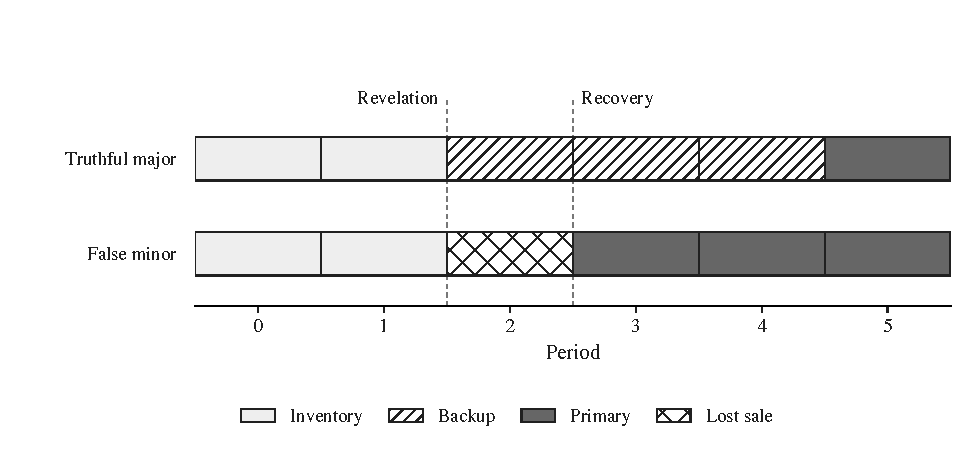
\includegraphics[width=\linewidth]{figures/mechanism.pdf}\caption{Demand fulfillment in the six-period lost-sales example, conditional on the long type. Each block represents one unit of demand. The truthful major notice induces qualification at period 0 and backup deliveries in periods 2--4. Under the false minor notice, the order due in period 2 fails, the report is exposed, and that period's demand is lost; the buyer does not qualify subsequently. Primary supply recovers in period 3. Backup displacement is 3 units, additional primary delivery is 2 units, and supplier gain is $2r-\kappa$ when $\lambda=1$ and $F=0$.}\label{fig:mechanism}
\ifprovenance\par\scriptsize Source SHA-256: \texttt{b8baea2609bdb4729a19b4dad71164f764149b25db58d3999e3225598ea03d9d}\par \texttt{58c2f08fa4ff92ca4492780fe81211d0508a5e855c0ea07dfe84aa6abd1ce3e1}\fi\end{figure}
% End mechanism.tex

% Begin parameter_map.tex
% Source SHA-256: b8baea2609bdb4729a19b4dad71164f764149b25db58d3999e3225598ea03d9d
\begin{figure}[htbp]\centering
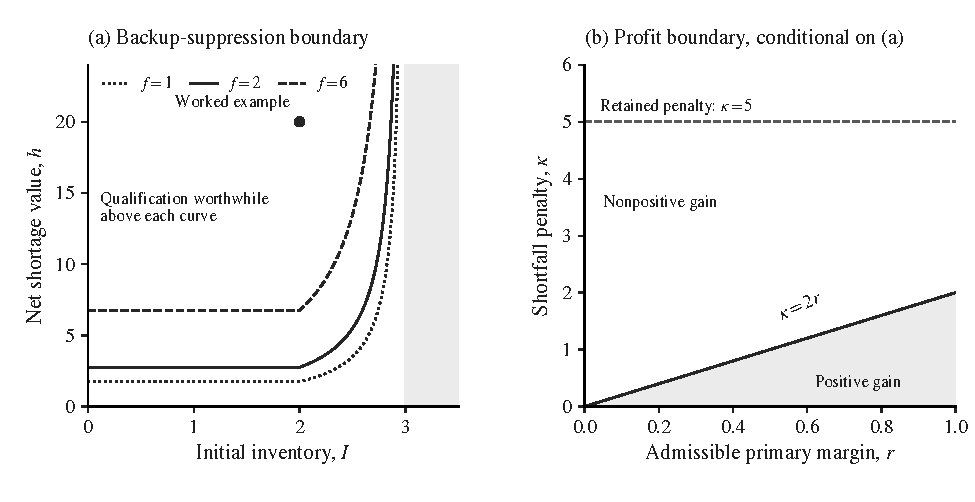
\includegraphics[width=\linewidth]{figures/parameter_map.pdf}
\caption{Analytical illustration of two separate boundaries. (a) With $H=6$, $D_S=2$, $D_L=3$, $L=2$, $K=3$, $p=1$ and $c_B=1.25$, suppression requires $h>(f+0.75)/\min\{(3-I)_+,1\}$; equality selects no qualification. The shaded inventory region has no avoided lost demand and the window is closed for every positive fee. Curves vary the fee while retaining the worked example's other primitives. (b) Conditional on the worked example's suppression outcome, $\Delta D=2$, $\Delta A=1$, $\lambda=1$ and $F=0$ give positive supplier gain only below $\kappa=2r$. With $p=1$ and nonnegative production cost, $0\le r\le1$. The retained penalty $\kappa=5$ lies above the profitable region throughout this range.}
\label{fig:parameter_map}\end{figure}
% Band-removal audit SHA-256: 7b8eb4e75ff493c920f95e0b1ae9511d9f872410fc04c0b30fbe36c6baf537c6
% End parameter_map.tex

% End section3.tex

% Begin section4.tex
\section{Network study design}\label{sec:design}
\subsection{A structural robustness population}
The network model adds product-specific inventories, assembly coefficients, accepted purchase orders, transport pipelines and alternative supply to the single-buyer benchmark. Each set has 56 cases: 24 window networks, eight boundary controls, and eight networks in each of three comparison regimes. For window networks, backup can arrive before recovery, but waiting for revelation misses the latest useful qualification date. The boundary controls close the opportunity with inventory or a fee. The comparison regimes have late backup, useful late backup, or alternative supply: backup arrives too late to rescue demand, remains useful after revelation, or competes with spot and stocked sources, respectively. Serial, assembly, distribution, layered and bypass-route families appear at small and large sizes. The bypass-route family combines a direct route to retail with a slower indirect route. Both finite and through-horizon commitments appear.

The horizon is 20 periods, primary price is one, backup price is 1.25, mandatory backup flow is one, and net shortage value is 20. The shortfall penalty is five. Supplier profitability is evaluated over ordinary nonnegative margins $0\le r\le p=\pc{rMax}$. Section~\ref{sec:estimands} and Supplement~G document the repricing of the preregistered financial contrast. The shortage value and penalty are modeling assumptions. Total demand is deterministically one unit per period. The specified qualification lead ends at the critical-part receiving site; additional transport to final demand is modeled separately.

Three combinations of the public timing and cost factors were specified before screening truthful-notice behavior. The screen required backup qualification on at least 12 of the 24 window networks under a truthful major notice for a long outage ($C_{00}$), with all 24 acceptable. Other outcomes did not affect selection. All three passed, so the first combination was selected by the prespecified rule. The resulting population deliberately emphasizes the suppression window. The full allocation and all three screen outcomes remain in Supplement~B.

The sealed confirmation set retained each case's regime, family, size, outage durations, qualification lead, inventory, fee and commitment. It redrew ordinary capacities, transport leads and costs, selected nodes, routes, outlets and demand shares within declared ranges. Template edges and the alternative-supply regime's supply options remained fixed. Each draw had to differ structurally from every public template and earlier accepted draw and be feasible without disruption. Qualification and reporting outcomes did not enter this filter. All 56 cases were audited against their preregistered structural requirements before analysis, and none could be dropped or replaced after opening. ``Structural confirmation'' refers to this conditional robustness exercise at fixed timing and cost parameters.

\subsection{Planner and interventions}
The receiver solves a rolling mixed-integer model each period and executes its current action. It observes current capacity and due obligations, updates after revelation, and plans future production and orders using its recovery belief and the deterministic demand sequence. Actual capacity governs the transition. A notice's schedule controls acceptance, and revelation corrects future acceptance without cancelling outstanding orders. Supplier damages are outside the buyer's objective.

The rolling mixed-integer program chooses primary orders, spot procurement, qualification, production and shipments under product-specific inventory and pipeline balances, assembly requirements, lane capacities and mandatory backup commitments. Decisions remain common across capacity scenarios until revelation. Its objective combines expected operating cost with a $10^{-3}$ current-action score that penalizes qualification now more strongly than the continuous controls. \ref{app:network_model} gives the model formulation and rolling update; Supplement~B supplies the full bounds, prime-root weights and numerical checks.

For an actual long outage, we cross the schedule and initial belief:
\begin{align*}
 C_{00}:&\ \text{major schedule, long belief},&
 C_{10}:&\ \text{minor schedule, long belief},\\
 C_{01}:&\ \text{major schedule, short belief},&
 C_{11}:&\ \text{minor schedule, short belief}.
\end{align*}
The same network and demand realization enter each cell. $C_{11}$ is the false minor notice believed literally until revelation; the mixed cells isolate the two report components. The four paired cells are evaluated on every design and confirmation network, with independent verification of actions and accounting.

False-notice outcomes on the public design set were used solely to validate the analysis pipeline and lock the precision forecast prior to opening the confirmation holdout, without altering hypotheses, test rules, or sample size. All 24 confirmation window networks entered the primary analysis with full independent verification.

\subsection{Estimands and conditional uncertainty}\label{sec:estimands}
For each network, $b=B_{00}-B_{11}$ is displaced backup, and $\Delta D=P_{11}-P_{00}$ is additional primary delivery. Supplier gain follows Equation~\eqref{eq:gain}. Buyer operating harm is $H=C_{11}-C_{00}$, with
\begin{align}
 H_C&=C_{10}-C_{00}, &H_B&=C_{01}-C_{00},\nonumber\\
 H_I&=C_{11}-C_{10}-C_{01}+C_{00}, &H&=H_C+H_B+H_I.\label{eq:channels}
\end{align}
Contractual, belief and interaction effects are paired operational contrasts and may have either sign.

The primary hypothesis requires positive means for both $b$ and $\Delta D$ among window networks, with both lower bounds of their two-sided 95\% intervals above zero. Outcomes are aggregated within networks, averaged within families, and then averaged with equal family weights. A family-stratified bootstrap uses 10,000 resamples; a network sign-flip check uses 100,000 draws, with disagreement reported as fragility without changing the primary decision. If this joint rule was satisfied, the preregistered analysis assessed three secondary contrasts using two-sided 98.33\% Bonferroni intervals: additional primary deliveries among window networks relative to the pooled comparison regimes, supplier gain $G(3,5)$, and buyer harm. The intervals summarize variation across the selected network cases conditional on the fixed allocation and structural draw process. The preregistered $G(3,5)$ contrast uses a margin above the unit purchase price and is retained as a historical score, not financial evidence. Post-confirmation repricing restricts $r$ to $[0,p]$; because $r$ enters neither the buyer objective nor its constraints, every physical action and buyer-cost contrast is unchanged. Corrected gain intervals are descriptive, pointwise 98.33\% intervals using the same resamples; the two retained secondary contrasts keep their original three-contrast adjustment. Supplement~B supplies the resampling details and seeds, and Supplement~G documents the correction.

\subsection{Ex ante commitment comparison}\label{sec:exante_design}
We compare both commitment rules on the same \xa{n} public design window networks, holding structure, prices, fees, demand and recovery times fixed within each pair. The declared grid is $\mu\in\{\xa{mu0},\xa{mu1},\xa{mu2},\xa{mu3},\xa{mu4}\}$ and $\beta\in\{\xa{beta0},\xa{beta1},\xa{beta2},\xa{beta3},\xa{beta4}\}$. Here $\mu$ is the probability of a long outage and $\beta$ is the specified probability that a long type reports minor; the short type reports minor. The same $\beta$ applies under both contracts, and the minor-notice posterior follows Equation~\eqref{eq:bayes}. Actual recovery is observed at revelation, and total demand remains at baseline (\xa{demand} unit per period) throughout.

For network $i$ and commitment $k$, the three realized operating costs are $C_{ik}^{S,m}(\alpha)$ for short/minor, $C_{ik}^{L,M}$ for truthful long/major with certain long belief, and $C_{ik}^{L,m}(\alpha)$ for long/minor. Expected buyer cost is
\begin{equation}
 \mathcal C_{ik}(\mu,\beta)=(1-\mu)C_{ik}^{S,m}(\alpha)
 +\mu(1-\beta)C_{ik}^{L,M}+\mu\beta C_{ik}^{L,m}(\alpha).
 \label{eq:exante_cost}
\end{equation}
Costs sum the operating charges in the executed-path ledgers, excluding the numerical tie term and penalty receipts. Relative to truthful reporting, the increase separates into
\begin{align}
 \mathcal C_{ik}(\mu,\beta)-\mathcal C_{ik}(\mu,0)
 ={}&(1-\mu)\big[C_{ik}^{S,m}(\alpha)-C_{ik}^{S,m}(1)\big]\nonumber\\
 &+\mu\beta\big[C_{ik}^{L,m}(\alpha)-C_{ik}^{L,M}\big].
 \label{eq:exante_split}
\end{align}
The first term is precautionary cost when the minor notice is true; the second is weighted harm from a false minor notice. We report within-network cost differences and equal-family means, with arithmetic means in Supplement~I. Conditional supplier gains use $r=\xa{r}$ and $\kappa=\xa{kappa}$. These gains diagnose the specified reporting behavior without determining it in equilibrium.


We also consider a hypothetical unconditional date-zero concession $\delta=\fd{delta}$ for choosing the through-horizon contract. For each network, the original and adjusted differences are
\begin{equation}\label{eq:fixed_discount}
 \Delta_i=\mathcal C_{i,\mathrm{hor}}-\mathcal C_{i,\mathrm{fin}},\qquad
 \Delta_i^\delta=\Delta_i-\delta,\qquad \delta_i^*=\Delta_i.
\end{equation}
Through-horizon commitment is preferred precisely when $\delta>\delta_i^*$; equality selects finite. The concession is fixed before operations and is independent of qualification and delivered volume. We subtract it from saved ex ante costs without recomputing physical policies. This buyer-side transfer leaves the incumbent's gain under each contract unchanged. Reporting likelihoods and Bayesian posteriors remain common across contracts, and the comparison remains post-confirmation exploratory.
% End section4.tex

% Begin section5.tex
\section{Structural robustness results}\label{sec:results}
\subsection{Backup displacement and additional primary delivery}
All \auditcount{confirmationInterior} window networks in the confirmation set have $b>0$ and $\Delta D>0$; the corresponding design count is also \auditcount{designInterior} of \auditcount{designInterior}. All selected backup under truthful major notices. Thus the delivery mechanism survives each sampled structural departure in the population of window networks.

Table~\ref{tab:table1} reports the equal-family estimates and intervals. Both primary lower bounds exceed zero, as do the retained secondary lower bounds for the delivery contrast and buyer harm. Corrected supplier profitability is evaluated separately in Section~\ref{sec:margin}.

Backup displacement and its interval match design exactly because retained timing and commitment factors determine the mandatory stream once qualification is unchanged. By contrast, the primary-delivery response depends on multi-tier network flows, shifting from a mean of \ev{t1r2c1n0} in design to \ev{t1r2c2n0} in confirmation to provide the informative structural replication (corroborated by the sign-flip sensitivity in Supplement~B).
% Begin table1.tex
% Sources: f1eef2f55a744295094897ce70a38f5b738ac3e41def05b6d53439fd0a41687b, bb0a2208ca1668198cdf09ff091d8cdf37fcbfbe0ec9baf8f5897cc0f51ed224
\begin{table}[!htbp]\centering\small
\setlength{\tabcolsep}{4pt}\renewcommand{\arraystretch}{1.18}\renewcommand{\thetable}{1}
\caption{Primary and retained secondary contrasts: confirmation and public design comparison.}\label{tab:table1}
\begin{tabular}{>{\raggedright\arraybackslash}p{6.2cm}>{\raggedright\arraybackslash}p{3.8cm}>{\raggedright\arraybackslash}p{3.8cm}}
\toprule
Contrast & Confirmation estimate [interval] & Design estimate [interval] \\
\midrule
Backup displacement, $b$ & 10.720 [8.280, 13.100] & 10.720 [8.280, 13.100] \\
Additional primary deliveries, $\Delta D$ & 9.076 [6.690, 11.421] & 9.035 [6.672, 11.367] \\
Additional deliveries: window networks versus comparison networks & 9.401 [6.460, 12.269] & 9.375 [6.456, 12.228] \\
Buyer harm, $C_{11}-C_{00}$ & 21.478 [16.838, 26.386] & 21.595 [17.032, 26.468] \\
\bottomrule\end{tabular}

\noindent\footnotesize Equal-family network means. Primary intervals are 95.00\%; the two reported secondary intervals retain the original three-contrast Bonferroni level of 98.33\%. Their lower bounds exceed zero. The original financial contrast is documented in Supplement~G; corrected profitability is reported separately in Table~\ref{tab:margin}.\par
\ifprovenance\noindent\scriptsize Source SHA-256: \texttt{f1eef2f55a744295094897ce70a38f5b738ac3e41def05b6d53439fd0a41687b}\par \texttt{bb0a2208ca1668198cdf09ff091d8cdf37fcbfbe0ec9baf8f5897cc0f51ed224}\par
\fi
\end{table}
% End table1.tex


\subsection{Why the contractual component is zero}
In the confirmation means for the window networks, both correct-belief cells cost \ev{t2r2c1}. Changing beliefs with the truthful schedule fixed raises cost by \ev{t2r2c6}; changing schedule and belief together adds an interaction of \ev{t2r2c7}. Total harm is \ev{t2r2c8}. The design attribution is similar (Figure~\ref{fig:harm_channels}, Table~\ref{tab:table2}).

The action and accounting comparison explains the zero contractual component. With correct long-outage beliefs, no newly accepted order is due before recovery; post-notice reliance shortfall is zero. The minor schedule's additional acceptance capacity is therefore unused. The two correct-belief cells execute numerically identical actions in both sets. Supplement~F records the action and accounting checks.

When the buyer instead expects early recovery, the schedule can affect its orders, producing the positive interaction. Correct beliefs eliminate the measured contract-only harm in these cases.
% Begin harm_channels.tex
% Source SHA-256: f1eef2f55a744295094897ce70a38f5b738ac3e41def05b6d53439fd0a41687b, 8d32d1127ecd229475305361a3bbb9fc434e2422c4057bfdd1120b4ead800040, bb0a2208ca1668198cdf09ff091d8cdf37fcbfbe0ec9baf8f5897cc0f51ed224, 7a0c0f4218632c47c75b511f76b8a19df0d0c42bbf06b0cbf77f969ade2a3ce1
\begin{figure}[htbp]\centering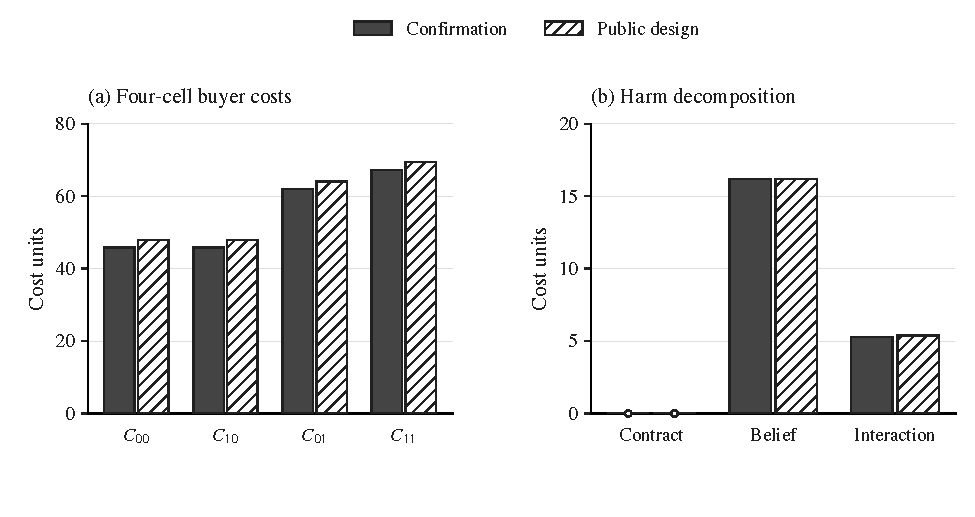
\includegraphics[width=\linewidth]{figures/harm_channels.pdf}\caption{Buyer costs and harm decomposition in window networks (equal-family means). The first subscript of $C$ changes the schedule from major to minor; the second changes the belief from long to short. Contractual harm is $C_{10}-C_{00}$, belief harm is $C_{01}-C_{00}$, and interaction is $C_{11}-C_{10}-C_{01}+C_{00}$. Contractual harm is zero in both sets, as indicated by the marks at the origin. Values are reproduced from Table~\ref{tab:table2}.}\label{fig:harm_channels}
\ifprovenance\par\scriptsize Source SHA-256: \texttt{f1eef2f55a744295094897ce70a38f5b738ac3e41def05b6d53439fd0a41687b}\par \texttt{8d32d1127ecd229475305361a3bbb9fc434e2422c4057bfdd1120b4ead800040}\par \texttt{bb0a2208ca1668198cdf09ff091d8cdf37fcbfbe0ec9baf8f5897cc0f51ed224}\par \texttt{7a0c0f4218632c47c75b511f76b8a19df0d0c42bbf06b0cbf77f969ade2a3ce1}\fi\end{figure}
% End harm_channels.tex

% Begin table2.tex
% Sources: f1eef2f55a744295094897ce70a38f5b738ac3e41def05b6d53439fd0a41687b, 8d32d1127ecd229475305361a3bbb9fc434e2422c4057bfdd1120b4ead800040, bb0a2208ca1668198cdf09ff091d8cdf37fcbfbe0ec9baf8f5897cc0f51ed224, 7a0c0f4218632c47c75b511f76b8a19df0d0c42bbf06b0cbf77f969ade2a3ce1
\begin{table}[!htbp]\centering\small
\setlength{\tabcolsep}{4pt}\renewcommand{\arraystretch}{1.18}\renewcommand{\thetable}{2}
\caption{Four-cell costs and harm decomposition, window networks.}\label{tab:table2}
\begin{tabular}{>{\raggedright\arraybackslash}p{6.2cm}>{\raggedright\arraybackslash}p{3.8cm}>{\raggedright\arraybackslash}p{3.8cm}}
\toprule
Measure & Confirmation & Design \\
\midrule
$C_{00}$: major schedule, long belief & 45.792 & 47.808 \\
$C_{10}$: minor schedule, long belief & 45.792 & 47.808 \\
$C_{01}$: major schedule, short belief & 61.968 & 64.008 \\
$C_{11}$: minor schedule, short belief & 67.270 & 69.403 \\
Contractual & 0.000 & 0.000 \\
Belief & 16.176 & 16.200 \\
Interaction & 5.302 & 5.395 \\
Total harm & 21.478 & 21.595 \\
\bottomrule\end{tabular}

\ifprovenance\noindent\scriptsize Source SHA-256: \texttt{f1eef2f55a744295094897ce70a38f5b738ac3e41def05b6d53439fd0a41687b}\par \texttt{8d32d1127ecd229475305361a3bbb9fc434e2422c4057bfdd1120b4ead800040}\par \texttt{bb0a2208ca1668198cdf09ff091d8cdf37fcbfbe0ec9baf8f5897cc0f51ed224}\par \texttt{7a0c0f4218632c47c75b511f76b8a19df0d0c42bbf06b0cbf77f969ade2a3ce1}\par\fi
\end{table}
% End table2.tex


\subsection{Controls and the long-outage reversal}
All eight inventory-closed and fee-closed controls skip backup and have zero displacement and primary-delivery change. Three fee-closed confirmation controls have small positive buyer harm, at most \ev{t3r3c7}. The prespecified control prediction concerns backup and displacement, so these costs are retained without relabeling the prediction. The full control rows appear in Supplement~E.

Table~\ref{tab:regime_compact} summarizes regimes; its combined row includes the eight boundary controls and therefore has a broader population than the primary analysis. In the late-backup and alternative-supply regimes, both reports skip backup. In the useful-late-backup regime, both select it, with changed timing. Confirmation buyer harm in that regime is \ev{t4r7c8}, while supplier gain at the illustrative margin $r=0.5$ is \mg{regime_confirmation_R3} and additional primary delivery is \ev{t4r7c6}. Backup still pays after revelation, so a false notice can delay useful mitigation without securing extra incumbent sales. This is the model's conditional long-outage reversal: harm remains large while the reporting deviation loses money.
% Begin regime_compact.tex
% Repriced gain source SHA-256: 7fcd4ca9507b14e6216945ff61db4019108c6f13122436ecf65bf83b63169fb6
% Sources: f1eef2f55a744295094897ce70a38f5b738ac3e41def05b6d53439fd0a41687b, bb0a2208ca1668198cdf09ff091d8cdf37fcbfbe0ec9baf8f5897cc0f51ed224
\begin{table}[!htbp]\centering\small
\setlength{\tabcolsep}{4pt}\renewcommand{\arraystretch}{1.18}\renewcommand{\thetable}{3}
\caption{Descriptive regime means. The combined group contains 24 window networks and eight boundary controls. Gain uses the illustrative midpoint $r=0.5$; Table~\ref{tab:margin} covers the admissible range. T/F denotes truthful-major / false-minor qualification counts.}\label{tab:regime_compact}
\begin{tabular}{>{\raggedright\arraybackslash}p{3.4cm}>{\raggedright\arraybackslash}p{0.5cm}>{\raggedright\arraybackslash}p{2.3cm}>{\raggedright\arraybackslash}p{1.3cm}>{\raggedright\arraybackslash}p{1.3cm}>{\raggedright\arraybackslash}p{1.6cm}>{\raggedright\arraybackslash}p{1.6cm}}
\toprule
Regime & $n$ & Backup selected T/F & $b$ & $\Delta D$ & $G(0.5,5)$ & Buyer harm \\
\midrule
\addlinespace\multicolumn{7}{l}{\textit{Confirmation}}\\
Window networks and controls & 32 & 24/0 & 8.031 & 6.793 & \mg{regime_confirmation_R1} & 16.248 \\
Late backup & 8 & 0/0 & 0.000 & 0.000 & \mg{regime_confirmation_R2} & 0.005 \\
Useful late backup & 8 & 8/8 & 0.750 & -0.625 & \mg{regime_confirmation_R3} & 26.270 \\
Alternative supply & 8 & 0/0 & 0.000 & -0.328 & \mg{regime_confirmation_R4} & 0.066 \\
\addlinespace\multicolumn{7}{l}{\textit{Design}}\\
Window networks and controls & 32 & 24/0 & 8.031 & 6.766 & \mg{regime_design_R1} & 16.302 \\
Late backup & 8 & 0/0 & 0.000 & 0.000 & \mg{regime_design_R2} & 0.005 \\
Useful late backup & 8 & 8/8 & 0.750 & -0.625 & \mg{regime_design_R3} & 27.214 \\
Alternative supply & 8 & 0/0 & 0.000 & -0.375 & \mg{regime_design_R4} & 0.075 \\
\bottomrule\end{tabular}

\ifprovenance\noindent\scriptsize Source SHA-256: \texttt{f1eef2f55a744295094897ce70a38f5b738ac3e41def05b6d53439fd0a41687b}\par \texttt{bb0a2208ca1668198cdf09ff091d8cdf37fcbfbe0ec9baf8f5897cc0f51ed224}\par
\fi
\end{table}
% End regime_compact.tex


\subsection{Descriptive variation within the window networks}
Table~\ref{tab:family_breakdown}, panels (a) and (b), partitions the same confirmation window networks by family and by commitment type. It reports group sizes and arithmetic means with observed minima and maxima for each delivery, payoff and harm component. The contractual component is zero throughout. These delivery and gain ranges describe groups that differ in commitment, timing, inventory and network structure.

The larger descriptive contrast is between commitment types. Each group contains \sr{n5} networks. Mean displaced backup is \sr{5_b_mean} in the finite-commitment group and \sr{6_b_mean} in the through-horizon group. Mean additional primary delivery is \sr{5_delta_d_mean} under finite commitment and \sr{6_delta_d_mean} through the horizon; mean supplier gain at $r=0.5$ is \mg{g5_mean} and \mg{g6_mean}, respectively. This midpoint illustrates the contrast; Table~\ref{tab:margin} and Figure~\ref{fig:margin} report the full margin range. Mean buyer harm is lower in the through-horizon group, at \sr{6_buyer_harm_mean} versus \sr{5_buyer_harm_mean}, despite its much larger supplier gain. Equation~\eqref{eq:displacement} explains the mechanism: backup units committed after primary recovery can replace incumbent sales, so suppressing a longer stream can retain more of those sales. The observed reporting gains are concentrated in the through-horizon group, while the buyer's loss persists under finite commitments.

The harm components also vary across families. Distribution networks have mean interaction harm of \sr{2_interaction_mean}, with observed range [\sr{2_interaction_min}, \sr{2_interaction_max}], alongside mean belief harm of \sr{2_belief_mean}. Mean interaction harm is \sr{0_interaction_mean} in Serial, \sr{3_interaction_mean} in Layered and \sr{1_interaction_mean} in Assembly networks. In the Distribution networks, opening retail stock serves local demand before any upstream arrival. Comparing the two false-belief cells, $C_{01}$ and $C_{11}$, changing the schedule leaves total primary deliveries and total lost sales unchanged; the small net cost difference is entirely transport cost. Thus the schedule changes some ordering and shipment timing without adding aggregate lost sales in these paths. Supplement~F records the paired cost accounting.

Across all \sr{balanceCases} confirmation window pairs, the multi-tier delivery balance satisfies $\Delta D=b-\widetilde u-\widetilde E$, where $\widetilde u$ is the increase in realized lost sales under the false notice and $\widetilde E$ is the truthful-minus-false difference in terminal stock (counting finished goods and critical inputs one-for-one). Multi-tier flows thus generalize the single-buyer identity in Equation~\eqref{eq:displacement}: serial paths introduce downstream stock, split retail demand, and post-receiving transit lags; assembly paths combine local conversion with downstream finished-goods shipments; distribution paths buffer split retail demand with opening local stock; and layered and bypass-route paths retain terminal critical-part stock under through-horizon commitments. Supplement~F reports the exact per-network balances.
% Begin family_breakdown.tex
% Repriced gain source SHA-256: 7fcd4ca9507b14e6216945ff61db4019108c6f13122436ecf65bf83b63169fb6
% Sources: f1eef2f55a744295094897ce70a38f5b738ac3e41def05b6d53439fd0a41687b, 8d32d1127ecd229475305361a3bbb9fc434e2422c4057bfdd1120b4ead800040, 11639536c750b1d85fedc763be1fc67f781a8cdc75611d02d2f5d19ba35986be, c6c9056671382246ea5ad56855731f9f5f054f628ba01faf198ce14758721bab
\begin{landscape}
\begingroup\fontsize{9.5}{11}\selectfont\setlength{\tabcolsep}{3pt}\renewcommand{\arraystretch}{1.25}\setlength{\LTcapwidth}{\linewidth}
\renewcommand{\thetable}{4}
\begin{longtable}{>{\raggedright\arraybackslash}p{2.5cm}>{\centering\arraybackslash}p{0.7cm}*{7}{>{\centering\arraybackslash}p{2.45cm}}}
\caption{Descriptive breakdown of the 24 confirmation window networks. Gain uses the illustrative midpoint $r=0.5$. Each group has a row of arithmetic means followed by a row of observed [minimum, maximum] ranges.}\label{tab:family_breakdown}\\
\toprule
Group & $n$ & $b$ & $\Delta D$ & $G(0.5,5)$ & Buyer harm & Contractual & Belief & Interaction\\\midrule
\endfirsthead
Group & $n$ & $b$ & $\Delta D$ & $G(0.5,5)$ & Buyer harm & Contractual & Belief & Interaction\\\midrule
\endhead\bottomrule\endfoot
\multicolumn{9}{l}{\textit{(a) By network family}}\\
Serial & \sr{n0} & \sr{0_b_mean} & \sr{0_delta_d_mean} & \mg{g0_mean} & \sr{0_buyer_harm_mean} & \sr{0_contractual_mean} & \sr{0_belief_mean} & \sr{0_interaction_mean} \\*
 &  & \mbox{[\sr{0_b_min}, \sr{0_b_max}]} & \mbox{[\sr{0_delta_d_min}, \sr{0_delta_d_max}]} & \mbox{[\mg{g0_min}, \mg{g0_max}]} & \mbox{[\sr{0_buyer_harm_min}, \sr{0_buyer_harm_max}]} & \mbox{[\sr{0_contractual_min}, \sr{0_contractual_max}]} & \mbox{[\sr{0_belief_min}, \sr{0_belief_max}]} & \mbox{[\sr{0_interaction_min}, \sr{0_interaction_max}]} \\\addlinespace[5pt]
Assembly & \sr{n1} & \sr{1_b_mean} & \sr{1_delta_d_mean} & \mg{g1_mean} & \sr{1_buyer_harm_mean} & \sr{1_contractual_mean} & \sr{1_belief_mean} & \sr{1_interaction_mean} \\*
 &  & \mbox{[\sr{1_b_min}, \sr{1_b_max}]} & \mbox{[\sr{1_delta_d_min}, \sr{1_delta_d_max}]} & \mbox{[\mg{g1_min}, \mg{g1_max}]} & \mbox{[\sr{1_buyer_harm_min}, \sr{1_buyer_harm_max}]} & \mbox{[\sr{1_contractual_min}, \sr{1_contractual_max}]} & \mbox{[\sr{1_belief_min}, \sr{1_belief_max}]} & \mbox{[\sr{1_interaction_min}, \sr{1_interaction_max}]} \\\addlinespace[5pt]
Distribution & \sr{n2} & \sr{2_b_mean} & \sr{2_delta_d_mean} & \mg{g2_mean} & \sr{2_buyer_harm_mean} & \sr{2_contractual_mean} & \sr{2_belief_mean} & \sr{2_interaction_mean} \\*
 &  & \mbox{[\sr{2_b_min}, \sr{2_b_max}]} & \mbox{[\sr{2_delta_d_min}, \sr{2_delta_d_max}]} & \mbox{[\mg{g2_min}, \mg{g2_max}]} & \mbox{[\sr{2_buyer_harm_min}, \sr{2_buyer_harm_max}]} & \mbox{[\sr{2_contractual_min}, \sr{2_contractual_max}]} & \mbox{[\sr{2_belief_min}, \sr{2_belief_max}]} & \mbox{[\sr{2_interaction_min}, \sr{2_interaction_max}]} \\\addlinespace[5pt]
Layered & \sr{n3} & \sr{3_b_mean} & \sr{3_delta_d_mean} & \mg{g3_mean} & \sr{3_buyer_harm_mean} & \sr{3_contractual_mean} & \sr{3_belief_mean} & \sr{3_interaction_mean} \\*
 &  & \mbox{[\sr{3_b_min}, \sr{3_b_max}]} & \mbox{[\sr{3_delta_d_min}, \sr{3_delta_d_max}]} & \mbox{[\mg{g3_min}, \mg{g3_max}]} & \mbox{[\sr{3_buyer_harm_min}, \sr{3_buyer_harm_max}]} & \mbox{[\sr{3_contractual_min}, \sr{3_contractual_max}]} & \mbox{[\sr{3_belief_min}, \sr{3_belief_max}]} & \mbox{[\sr{3_interaction_min}, \sr{3_interaction_max}]} \\\addlinespace[5pt]
Bypass-route & \sr{n4} & \sr{4_b_mean} & \sr{4_delta_d_mean} & \mg{g4_mean} & \sr{4_buyer_harm_mean} & \sr{4_contractual_mean} & \sr{4_belief_mean} & \sr{4_interaction_mean} \\*
 &  & \mbox{[\sr{4_b_min}, \sr{4_b_max}]} & \mbox{[\sr{4_delta_d_min}, \sr{4_delta_d_max}]} & \mbox{[\mg{g4_min}, \mg{g4_max}]} & \mbox{[\sr{4_buyer_harm_min}, \sr{4_buyer_harm_max}]} & \mbox{[\sr{4_contractual_min}, \sr{4_contractual_max}]} & \mbox{[\sr{4_belief_min}, \sr{4_belief_max}]} & \mbox{[\sr{4_interaction_min}, \sr{4_interaction_max}]} \\\addlinespace[5pt]
\multicolumn{9}{l}{\textit{(b) By commitment type}}\\
Finite & \sr{n5} & \sr{5_b_mean} & \sr{5_delta_d_mean} & \mg{g5_mean} & \sr{5_buyer_harm_mean} & \sr{5_contractual_mean} & \sr{5_belief_mean} & \sr{5_interaction_mean} \\*
 &  & \mbox{[\sr{5_b_min}, \sr{5_b_max}]} & \mbox{[\sr{5_delta_d_min}, \sr{5_delta_d_max}]} & \mbox{[\mg{g5_min}, \mg{g5_max}]} & \mbox{[\sr{5_buyer_harm_min}, \sr{5_buyer_harm_max}]} & \mbox{[\sr{5_contractual_min}, \sr{5_contractual_max}]} & \mbox{[\sr{5_belief_min}, \sr{5_belief_max}]} & \mbox{[\sr{5_interaction_min}, \sr{5_interaction_max}]} \\\addlinespace[5pt]
Through horizon & \sr{n6} & \sr{6_b_mean} & \sr{6_delta_d_mean} & \mg{g6_mean} & \sr{6_buyer_harm_mean} & \sr{6_contractual_mean} & \sr{6_belief_mean} & \sr{6_interaction_mean} \\*
 &  & \mbox{[\sr{6_b_min}, \sr{6_b_max}]} & \mbox{[\sr{6_delta_d_min}, \sr{6_delta_d_max}]} & \mbox{[\mg{g6_min}, \mg{g6_max}]} & \mbox{[\sr{6_buyer_harm_min}, \sr{6_buyer_harm_max}]} & \mbox{[\sr{6_contractual_min}, \sr{6_contractual_max}]} & \mbox{[\sr{6_belief_min}, \sr{6_belief_max}]} & \mbox{[\sr{6_interaction_min}, \sr{6_interaction_max}]} \\\addlinespace[5pt]
\end{longtable}
\noindent\footnotesize Family and commitment panels are separate partitions of the same window networks. Means within each group use equal network weights. Ranges describe the observed cases.\par
\endgroup\end{landscape}
% End family_breakdown.tex


\subsection{Supplier profitability over admissible margins}\label{sec:margin}
With purchase price one and nonnegative production cost, an ordinary nonnegative supplier margin lies in $[0,1]$. Table~\ref{tab:margin} reprices the saved paths at the five declared headline levels. The benchmark penalty is $\kappa=\pc{kappa}$ per unit of accepted-order shortfall. Relative to the assumed net shortage value $h=\pc{h}$, it is a \pc{damagesShare} share. This illustrative reliance-damages benchmark represents partial compensation for exposure to a failed commitment. It is assessed on accepted shortfall; inventory and alternative supply can separate a failed delivery from a lost sale. Figure~\ref{fig:incentive_map} extends the analysis across penalty levels, mapping the exact $(\kappa,r)$ regions where understatement is profitable without altering the physical primary trajectories or buyer-harm results.

The equal-family confirmation mean crosses zero at approximately $r=\mg{confirmationMeanRoot}$; its pointwise lower interval endpoint crosses zero near $r=\mg{confirmationLowerRoot}$ (Figure~\ref{fig:margin}). At $r=\mg{r2}$, mean gain is \mg{confirmation_2_mean_gain}, with pointwise interval [\mg{confirmation_2_lower_98_33}, \mg{confirmation_2_upper_98_33}]. At the upper admissible margin, it is \mg{confirmation_4_mean_gain}, with interval [\mg{confirmation_4_lower_98_33}, \mg{confirmation_4_upper_98_33}]. At the midpoint, \mg{positive2} of the \auditcount{confirmationInterior} window networks have positive gain. The design estimates follow the same pattern.

The descriptive mean gains differ by commitment type across this range. The finite-commitment mean stays negative even at $r=1$, where it is \mg{finite_4}. The through-horizon mean is \mg{horizon_2} at the midpoint and \mg{horizon_4} at the upper endpoint. Additional post-recovery sales can sustain profit when liability is spread over a longer displaced stream. The groups differ in other factors. Section~\ref{sec:paired} isolates the commitment change within each public design network.

Critical penalties also depend on the margin. At the illustrative midpoint, \mg{critconfirmation2c0} of all 56 confirmation cases have a finite profitable penalty range, with thresholds from \mg{critconfirmation2s0} to \mg{critconfirmation2s2} and median \mg{critconfirmation2s1}. Supplement~G reports every category at every headline margin. Where shortfall is zero, a penalty threshold is undefined and the gain sign is reported instead.
% Begin margin_table.tex
% Source SHA-256: 947873d38019dda675fd3c1f942145e7ecb069e9239c77f2a11a75aa68cb9904
\begin{table}[!htbp]\centering\small
\setlength{\tabcolsep}{3pt}\renewcommand{\arraystretch}{1.18}\renewcommand{\thetable}{5}
\caption{Post-confirmation supplier-margin repricing at penalty five.}\label{tab:margin}
\begin{tabular}{>{\raggedright\arraybackslash}p{1.3cm}>{\raggedright\arraybackslash}p{4.8cm}>{\raggedright\arraybackslash}p{4.8cm}>{\raggedright\arraybackslash}p{2.6cm}}
\toprule
Margin $r$ & \shortstack[l]{Confirmation mean\\\mbox{[98.33\% interval]}} & \shortstack[l]{Design mean\\\mbox{[98.33\% interval]}} & Positive confirmation cases \\
\midrule
\mg{r0} & \mg{confirmation_0_mean_gain} [\mg{confirmation_0_lower_98_33}, \mg{confirmation_0_upper_98_33}] & \mg{design_0_mean_gain} [\mg{design_0_lower_98_33}, \mg{design_0_upper_98_33}] & \mg{positive0}/\auditcount{confirmationInterior} \\
\mg{r1} & \mg{confirmation_1_mean_gain} [\mg{confirmation_1_lower_98_33}, \mg{confirmation_1_upper_98_33}] & \mg{design_1_mean_gain} [\mg{design_1_lower_98_33}, \mg{design_1_upper_98_33}] & \mg{positive1}/\auditcount{confirmationInterior} \\
\mg{r2} & \mg{confirmation_2_mean_gain} [\mg{confirmation_2_lower_98_33}, \mg{confirmation_2_upper_98_33}] & \mg{design_2_mean_gain} [\mg{design_2_lower_98_33}, \mg{design_2_upper_98_33}] & \mg{positive2}/\auditcount{confirmationInterior} \\
\mg{r3} & \mg{confirmation_3_mean_gain} [\mg{confirmation_3_lower_98_33}, \mg{confirmation_3_upper_98_33}] & \mg{design_3_mean_gain} [\mg{design_3_lower_98_33}, \mg{design_3_upper_98_33}] & \mg{positive3}/\auditcount{confirmationInterior} \\
\mg{r4} & \mg{confirmation_4_mean_gain} [\mg{confirmation_4_lower_98_33}, \mg{confirmation_4_upper_98_33}] & \mg{design_4_mean_gain} [\mg{design_4_lower_98_33}, \mg{design_4_upper_98_33}] & \mg{positive4}/\auditcount{confirmationInterior} \\
\bottomrule\end{tabular}
\par\medskip\parbox{\linewidth}{\footnotesize Equal-family window-network means. Pointwise 98.33\% intervals reuse the original paired bootstrap draws. They are descriptive, are not simultaneous across margins, and issue no new confirmatory decision. The purchase price is one; nonnegative production costs restrict the margin to $0\le r\le1$.}
\end{table}
% End margin_table.tex

% Begin margin_figure.tex
% Sources: 947873d38019dda675fd3c1f942145e7ecb069e9239c77f2a11a75aa68cb9904, 7fcd4ca9507b14e6216945ff61db4019108c6f13122436ecf65bf83b63169fb6, 5131f447a4adcdd3fd489f9126d1d5524bf1a90b9fa017d4630f08afe9f21295
\begin{figure}[!htbp]\centering
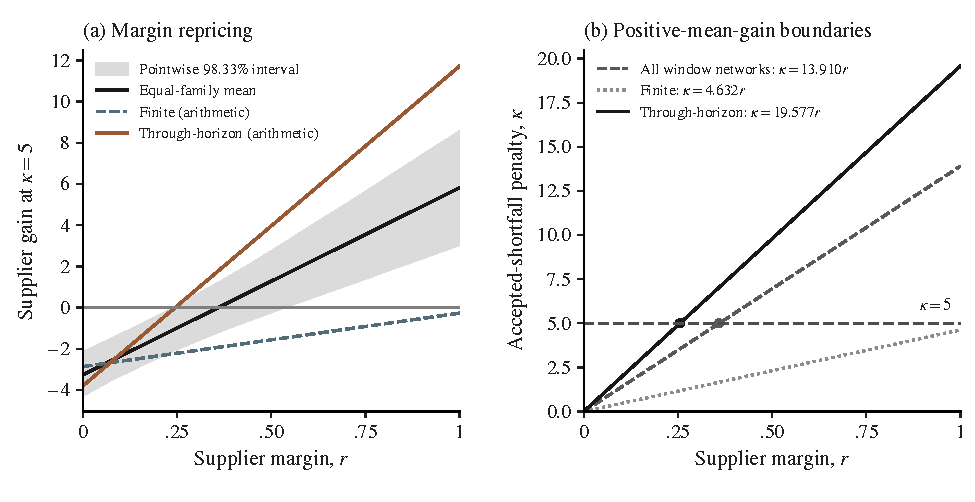
\includegraphics[width=\linewidth]{figures/profitability_combined.pdf}
\caption{(a) Post-confirmation repricing of the saved paths at penalty five. The purchase price is one. Equal-family confirmation mean and pointwise 98.33\% interval; arithmetic confirmation means by commitment, with 12 cases per group. The physical policies and buyer costs are unchanged. (b) Positive-mean-gain boundaries for confirmation window networks under full belief, using equal-family weights within each group. Mean gain is positive strictly below each line and zero on it. The horizontal line retains $\kappa=\pc{kappa}$. The commitment groups retain their original factors and structures; Section~\ref{sec:paired} separately changes commitment within each public design network.}\label{fig:profitability_combined}
\begingroup\makeatletter
\edef\@currentlabel{\thefigure a}\label{fig:margin}
\edef\@currentlabel{\thefigure b}\label{fig:incentive_map}
\makeatother\endgroup
\end{figure}
% End margin_figure.tex


The incentive map uses the same confirmation window networks and equal-family weights within each commitment group. Mean gain is positive when $\kappa<\pc{slopeall}r$ overall, $\kappa<\pc{slopefinite}r$ for finite commitments and $\kappa<\pc{slopehorizon}r$ for through-horizon commitments. At $\kappa=\pc{kappa}$, the overall and through-horizon means become positive above approximately $r=\pc{rootall}$ and $r=\pc{roothorizon}$, respectively. The finite-group zero crossing is $r\approx\pc{rootfinite}$, outside the admissible range. Lower penalties can therefore make finite commitments profitable even though their mean remains negative at the retained benchmark. These exact affine boundaries reprice the confirmation trajectories under full belief.

\subsection{Controlled commitment comparison}\label{sec:paired}
Each of the \pc{n} public design window networks receives finite and through-horizon backup commitments, changing only the commitment rule. Structure, supplier costs, demand, recovery times and buyer beliefs are held fixed within each pair, and qualification remains optional. Total demand remains at baseline (\pc{demand} unit per period) across all four schedule--belief cells and tested fractional beliefs. Every false-notice trajectory is benchmarked against truthful $C_{00}$ under the same commitment rule, isolating the ceteris paribus effect of commitment duration across the public design networks.

At $\kappa=\pc{kappa}$ under full belief, truthful qualification and its date remain unchanged in all \pc{truthUnchanged} networks. The longer commitment turns \pc{pair4_nonpositive_to_positive_count} networks from non-positive to positive supplier gain at every tested $r\geq\pc{switchStart}$, through $r=\pc{rMax}$. There are \pc{reverseMax} reverse switches anywhere in the tested belief, margin and penalty grid. Table~\ref{tab:paired} reports equal-family means at $r=\pc{rHalf}$. Accepted shortfall is equal under both contracts for every full-belief pair, so the gain difference comes entirely from $\Delta D$: mean additional primary delivery rises from \pc{finite4_mean_delta_d} to \pc{horizon4_mean_delta_d}, and mean gain rises from \pc{finite4_mean_gain} to \pc{horizon4_mean_gain}. Longer commitments displace more of the incumbent's post-recovery deliveries. Buyer harm falls from \pc{finite4_mean_buyer_harm} to \pc{horizon4_mean_buyer_harm}, measured relative to each contract's own truthful cost.
% Begin paired_table.tex
% Source SHA-256: e2cab9704d002158e0b7c75a1ce86356b5124c1949445437ce2ba68e3de1968f
\begin{table}[!htbp]\centering\small
\renewcommand{\thetable}{6}\setlength{\tabcolsep}{5pt}\renewcommand{\arraystretch}{1.2}
\caption{Controlled commitment comparison on the \pc{n} public design window networks under full belief. Equal-family means at $r=\pc{rHalf}$ and $\kappa=\pc{kappa}$.}\label{tab:paired}
\begin{tabular}{lrrrrr}\toprule
Commitment & $b$ & $\Delta D$ & Accepted shortfall & $G(\pc{rHalf},\pc{kappa})$ & Buyer harm\\\midrule
Finite & \pc{finite4_mean_b} & \pc{finite4_mean_delta_d} & \pc{finite4_mean_accepted_shortfall} & \pc{finite4_mean_gain} & \pc{finite4_mean_buyer_harm}\\
Through-horizon & \pc{horizon4_mean_b} & \pc{horizon4_mean_delta_d} & \pc{horizon4_mean_accepted_shortfall} & \pc{horizon4_mean_gain} & \pc{horizon4_mean_buyer_harm}\\
\bottomrule\end{tabular}
\par\medskip\parbox{\linewidth}{\footnotesize Each network receives both commitment rules. Each false-minor path is compared with truthful $C_{00}$ under the same rule. Accepted shortfall excludes the pre-horizon order. This is a descriptive controlled comparison within the declared model.}
\end{table}
% End paired_table.tex


The result changes with belief. At $\alpha=\pc{alpha2}$, $r=\pc{rHalf}$ and $\kappa=\pc{kappa}$, \pc{pair2_nonpositive_to_positive_count} networks switch into positive gain, while the longer-contract mean remains \pc{horizon2_mean_gain}, compared with \pc{finite2_mean_gain} under finite commitment. At $\alpha=\pc{alpha3}$, \pc{pair3_nonpositive_to_positive_count} networks switch and mean gain rises from \pc{finite3_mean_gain} to \pc{horizon3_mean_gain}. Mean buyer harm also rises at these weaker beliefs, by \pc{pair2_mean_change_buyer_harm} and \pc{pair3_mean_change_buyer_harm}, respectively. Thus the full-belief reduction in buyer harm does not extend to every belief. Figure~\ref{fig:paired_switches} gives the tested margin-dependent switch counts. Supplement~H lists every network; the accompanying files retain every belief, margin and penalty level.
% Begin paired_switches.tex
% Source SHA-256: e2cab9704d002158e0b7c75a1ce86356b5124c1949445437ce2ba68e3de1968f
\begin{figure}[!htbp]\centering
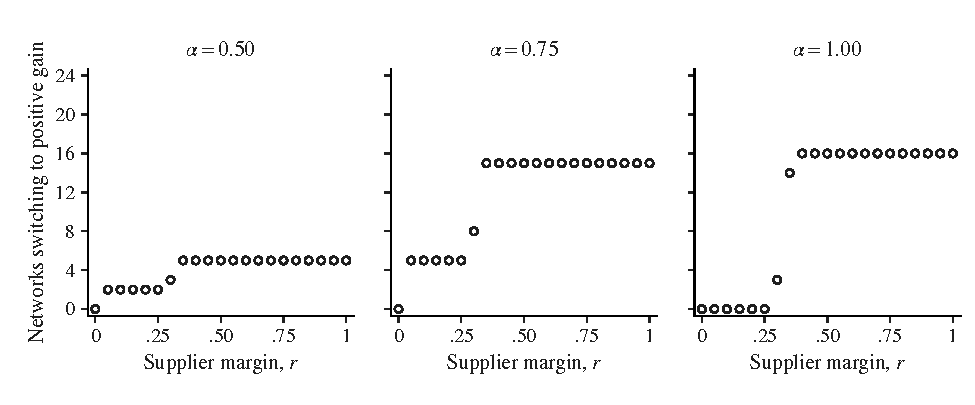
\includegraphics[width=\linewidth]{figures/paired_switches.pdf}
\caption{Networks whose gain changes from non-positive under finite commitment to positive under through-horizon commitment at $\kappa=\pc{kappa}$. Markers show the tested margins, spaced by \pc{rStep}; no between-level threshold is inferred. Reverse switches number \pc{reverseMax} throughout the complete tested belief, margin and penalty grid.}\label{fig:paired_switches}
\end{figure}
% End paired_switches.tex


\clearpage
\subsection{Ex ante commitment choice}\label{sec:exante}
Each of the \xa{n} public design window networks receives both commitment rules. To evaluate how reporting reliability shapes contract selection prior to a disruption, we evaluate both commitment rules across the $(\mu,\beta)$ outage-prior and reporting-likelihood grid defined in Section~\ref{sec:exante_design}.

Finite commitment is cheaper in \xa{finiteCheaper} of \xa{comparisons} network--probability comparisons and ties in \xa{ties}; through-horizon commitment is never cheaper. The longer contract raises conditional supplier gain in \xa{gainRaised} comparisons and leaves it unchanged in \xa{gainUnchanged}. Figure~\ref{fig:ex_ante}a shows the equal-family differences at equal contract prices. Under those prices, finite commitment weakly lowers both buyer cost and the supplier's incentive to misreport throughout this grid.
% Begin ex_ante_figure.tex
% Source SHA-256: de8810d45034f4d665cd18eb6cdd9892d9424abdfe7e978ec00daeb48b625c40; discount specification: 06e8a77742037508c31046219c09ff4b7b29692fe3bc7b852dfd278f2fe3f990
\begin{figure}[!htbp]\centering
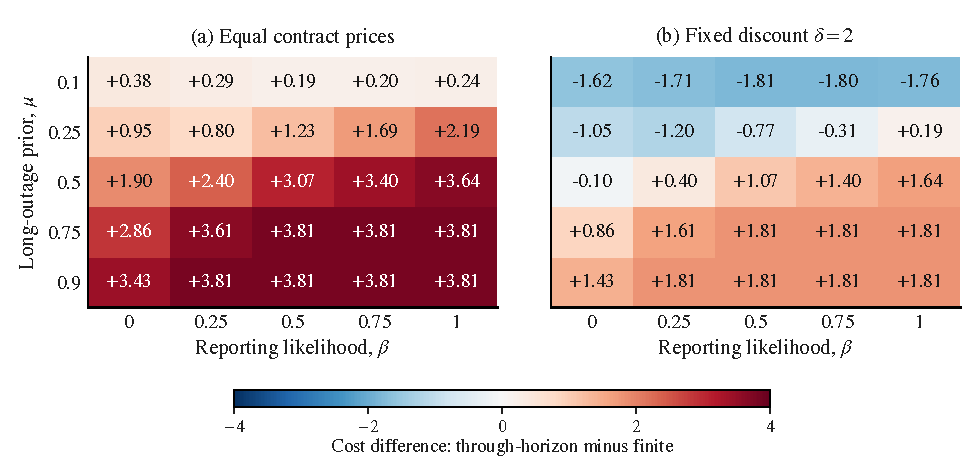
\includegraphics[width=\linewidth]{figures/fixed_discount_heatmap.pdf}
\caption{Equal-family expected-cost differences on the tested probability grid. Negative values favor through-horizon commitment; positive values favor finite commitment. Panel (b) subtracts an unconditional date-zero concession of $\delta=\fd{delta}$ from the saved costs in panel (a). This is a deterministic price adjustment, with no new simulation or equilibrium calculation.}\label{fig:ex_ante}
\end{figure}
% End ex_ante_figure.tex


The cost gap combines the premium already present under truthful reporting with the additional cost of possible misreporting. At $\mu=\xa{mu2}$, the gap rises from \xa{baseGap} at $\beta=\xa{beta0}$ to \xa{endGap} at $\beta=\xa{beta4}$. The added \xa{addedGap} comprises \xa{addedPrecaution} of extra precautionary cost and \xa{addedMisreport} of extra weighted false-notice harm, using Equation~\eqref{eq:exante_split}. At the latter endpoint, the weighted precautionary cost when the short notice is true is \xa{precFinite} under finite commitment and \xa{precHorizon} under through-horizon commitment.

The break-even up-front discount is $\delta^*=\mathcal C_{\mathrm{hor}}-\mathcal C_{\mathrm{fin}}$. A discount above $\delta^*$ makes through-horizon commitment preferable; equality retains finite under the declared tie rule. Equal-family discounts range from \xa{discountMin} to \xa{discountMax}. At $\mu=\xa{mu2}$ the required discount increases with $\beta$, from \xa{baseGap} to \xa{endGap}. The pattern is not universal: at $\mu=\xa{mu0}$ it initially falls from \xa{lowBaseGap} to \xa{lowMidGap}, then rises to \xa{lowEndGap}. Supplement~I retains both weighting schemes and every tested combination.


\paragraph{Contract preferences under a fixed price concession}
The equal-price result depends on the contract's financial terms. Subtracting the illustrative unconditional concession $\delta=\fd{delta}$ makes through-horizon commitment preferable in \fd{eq_horizon_after} of the \fd{eq_cells} equal-family mean comparisons (Figure~\ref{fig:ex_ante}b). At $\mu=\xa{mu2}$ and $\beta=\xa{beta0}$, the mean gap falls from \fd{low_original} to \fd{low_adjusted}, favoring through-horizon commitment. At $\beta=\xa{beta4}$ it falls from \fd{high_original} to \fd{high_adjusted}, leaving finite commitment preferable. A fixed price advantage can therefore be outweighed by the operating consequences of less reliable recovery information.

Aggregate preference differs from individual choice. The concession switches \fd{switches} of the \fd{network_comparisons} network--probability comparisons to through-horizon commitment; \fd{finite_after} retain finite, including \fd{ties_after} exact ties. At $\mu=\xa{mu2}$ and $\beta=\xa{beta0}$, \fd{low_horizon_after} networks favor through-horizon and \fd{low_finite_after} retain finite, including \fd{low_ties_after} ties; at $\beta=\xa{beta4}$ all retain finite. Supplement~I reports every combination. The concession changes the buyer's contract preference; it leaves each contract's physical policy and the incumbent's conditional reporting gain unchanged.
% End section5.tex

% Begin section6.tex
\section{Descriptive sensitivity}\label{sec:sensitivity}
\subsection{Demand persistence, alternatives and prices}
Supplement~E reports physical summaries for all declared arms and levels on the 56 public design cases; Table~\sensitivitySupplementNumber\ uses the illustrative midpoint $r=0.5$. Corrected supplier gains across the full margin range appear in Supplement~G; all sensitivity arms were prespecified for descriptive comparison on the public design set.

Allowing backlog with catch-up capacity 0.5 and unit backlog cost one lowers mean gain from \mg{sens0} to \mg{sens1}. Displacement falls from \ev{t6r1c1n0} to \ev{t6r2c1n0}. Some terminal backlog remains, so this is a finite-horizon comparison. A broker spot option with capacity 0.5 and price six in the window networks and the late-backup and useful-late-backup regimes lowers gain to \mg{sens2}. A contradiction cost of three reduces supplier gain without changing the buyer's actions; removing damages raises it to \mg{sens4}. Backup price parity leaves the baseline delivery summaries unchanged while changing buyer costs.

Expediting advances long-type recovery by one period at cost three. Within each cell, the supplier compares $rP-5A-3$ with the no-expedite payoff $rP-5A$, selecting expedite only when its net payoff exceeds the no-expedite payoff by more than the tolerance specified in Supplement~D; ties select no expedite. The independently checked saved alternatives select the same options throughout $r\in[0,1]$: one late-backup network expedites, in $C_{11}$. 

\subsection{Shortage value and the analytical boundary}
The baseline's $h=20$ is an assumed net shortage value for a critical part. In an automotive sequencing case, \citet[Section 4]{kang2018sequencing} report an OEM line-stoppage estimate of US\$\eqv{lineStopCost} per minute, dominated by labour costs. Figure~\ref{fig:parameter_map} displays the analytical cost boundaries. At $h=1$, mean displacement and supplier gain are \ev{t6r8c1n0} and \mg{sens7}; at $h=3$ they are \ev{t6r9c1n0} and \mg{sens8}; at $h=10$ they are \ev{t6r10c1n0} and \mg{sens9}. Backup displacement persists at $h=3$ even though mean supplier gain is negative. Early activation must avert enough lost demand to pay for the fee and the entire mandatory stream. The assumed margin and penalty then determine profitability through a different inequality.

Agreement between the single-buyer qualification prediction and the network planner is \ev{t7r8c5}, \ev{t7r9c5}, \ev{t7r10c5} and \ev{t7r1c5} at $h=1,3,10,20$, respectively (Supplement~E, Figure~\windowSupplementNumber).

\subsection{Discounted belief in the notice}\label{sec:discounted_belief}
All \db{designN} public design cases retain their originally assigned commitment, a long actual outage and a minor acceptance schedule. The buyer starts with $P(\mathrm{short})=\alpha$, where $\alpha\in\{\db{alpha0},\db{alpha1},\db{alpha2},\db{alpha3},\db{alpha4}\}$, and assigns certainty to the long outage at revelation. The endpoints $\alpha=\db{alpha0}$ and $\alpha=\db{alpha4}$ correspond to $C_{10}$ and $C_{11}$. The planner, tie convention and solver settings are unchanged. The sweep sets $\alpha$ exogenously. Equation~\eqref{eq:bayes} maps each tested value to combinations of a severity prior and an assumed lying rate.

Table~\ref{tab:discounted_belief} shows the response. Backup is suppressed when truthful $C_{00}$ selects qualification and the discounted-belief path ($\alpha$) selects none. Among window networks, none is suppressed at $\alpha=\db{alpha0}$ or $\db{alpha1}$, \db{s0a2} are suppressed at $\db{alpha2}$, \db{s0a3} at $\db{alpha3}$, and all \db{interiorN} at $\db{alpha4}$. Suppression and joint positivity of $b$ and $\Delta D$ occur at the same tested levels in every network, and every pattern is monotone in $\alpha$. No boundary control or comparison-regime case meets either condition at any level.

Mean gain among window networks at $r=0.5$ is $\mg{db1}$ at $\alpha=\db{alpha1}$: accepted shortfall increases without additional primary delivery. It remains negative at $\alpha=\db{alpha2}$, at $\mg{db2}$, and becomes positive at $\alpha=\db{alpha3}$, at $\mg{db3}$. The table reports every tested level alongside displacement, additional delivery and buyer harm; Supplement~G reports gains across margins. Thus the onset of suppression and the onset of positive mean profit differ.

The mechanism requires a receiver that puts substantial weight on the notice. No window network is suppressed at $\alpha=\db{alpha0}$ or $\db{alpha1}$; \db{fullOnly} of the \db{interiorN} window networks are suppressed only under full belief. The table reports arithmetic means for the public design cases.
% Begin discounted_belief_table.tex
% Repriced gain source SHA-256: 4a167dd25743218d59231709e5c75934fc156ae2fe64d65c1bc2e3961f6e4fba
% Sources: 1b262e14552a24ab4fcb808a3cbc1d33f6f48423b7e178665940addb94f912f1, 59bfcfc8a608e7f857080ea0e6fd08a5d46a586565d3ef115bcaddc3ec1ae00c, 6f9f7d4c6dc33aeef500ef35aa8bfd1c0f136badc46d2846a670db137717c891, a2848152c7bfb7cc425ddeb71bfe41e6b78476db847cc39a8e89af009a96a5d1
\begin{table}[htbp]
\centering\small\renewcommand{\thetable}{7}
\setlength{\tabcolsep}{5pt}\renewcommand{\arraystretch}{1.18}
\caption{Discounted belief in the notice: public design cases. Gain uses the illustrative midpoint $r=0.5$. Suppression means that $C_{00}$ selects qualification and the $\alpha$ path selects none.}
\label{tab:discounted_belief}
\begin{tabular}{lrrrrrr}
\toprule
\multicolumn{7}{l}{(a) Networks with backup suppressed}\\
Group & $n$ & $\alpha=\db{alpha0}$ & $\alpha=\db{alpha1}$ & $\alpha=\db{alpha2}$ & $\alpha=\db{alpha3}$ & $\alpha=\db{alpha4}$ \\
\midrule
Window networks & \db{n0} & \db{s0a0} & \db{s0a1} & \db{s0a2} & \db{s0a3} & \db{s0a4} \\
Boundary controls & \db{n1} & \db{s1a0} & \db{s1a1} & \db{s1a2} & \db{s1a3} & \db{s1a4} \\
Late backup & \db{n2} & \db{s2a0} & \db{s2a1} & \db{s2a2} & \db{s2a3} & \db{s2a4} \\
Useful late backup & \db{n3} & \db{s3a0} & \db{s3a1} & \db{s3a2} & \db{s3a3} & \db{s3a4} \\
Alternative supply & \db{n4} & \db{s4a0} & \db{s4a1} & \db{s4a2} & \db{s4a3} & \db{s4a4} \\
\bottomrule
\end{tabular}\par\medskip
\begin{tabular}{rrrrr}
\toprule
\multicolumn{5}{l}{(b) Window networks: arithmetic network means}\\
$\alpha$ & $b$ & $\Delta D$ & $G(0.5,5)$ & Buyer harm\\
\midrule
\db{alpha0} & \db{b0} & \db{d0} & \mg{db0} & \db{harm0} \\
\db{alpha1} & \db{b1} & \db{d1} & \mg{db1} & \db{harm1} \\
\db{alpha2} & \db{b2} & \db{d2} & \mg{db2} & \db{harm2} \\
\db{alpha3} & \db{b3} & \db{d3} & \mg{db3} & \db{harm3} \\
\db{alpha4} & \db{b4} & \db{d4} & \mg{db4} & \db{harm4} \\
\bottomrule\end{tabular}
\end{table}
% End discounted_belief_table.tex

% End section6.tex

% Begin section7.tex
\section{Discussion}\label{sec:discussion}
\paragraph{Post-recovery substitution and backup commitment design}
Whether a supplier profits from understating a disruption depends on what a backup commitment does \emph{after} the incumbent recovers. Backup units arriving during the outage rescue demand that the incumbent would otherwise lose permanently, whereas units arriving after recovery displace the incumbent's own post-recovery sales. Because the buyer pays for both streams under a mandatory commitment, the incumbent profits only from suppressing the post-recovery substitution component, net of shortfall liability. This accounting distinction explains why operational backup suppression, buyer harm, and supplier profit require separate measures and why backup commitment duration is a primary contract-design lever.

In our controlled comparison across the \pc{n} public design window networks, extending the backup contract from a finite commitment to a through-horizon commitment leaves truthful qualification timing and accepted-order shortfalls unchanged, but substantially increases the post-recovery primary deliveries retained when backup is suppressed. At $\kappa=\pc{kappa}$ under full belief, this post-recovery volume shifts \pc{pair4_nonpositive_to_positive_count} networks from non-positive to strictly positive supplier gain at every tested margin from \pc{switchStart} upward. Procurement managers negotiating backup supply agreements should therefore distinguish commitments needed to bridge an active outage from multi-period volume guarantees that persist long after primary recovery. Shorter commitments sharply curtail the incumbent's incentive to understate recovery dates, though buyers still face substantial operating losses if a false notice delays activation. The relative buyer harm under finite versus through-horizon rules depends on belief updating: longer commitments lower measured harm under full belief but increase mean harm under partial skepticism ($\alpha=\pc{alpha2}$ and $\alpha=\pc{alpha3}$), demonstrating that contract duration and timely recovery verification address complementary dimensions of disruption risk.

\paragraph{Ex ante pricing concessions versus information reliability}
When backup suppliers offer unconditional upfront price concessions for longer volume commitments, the buyer's ex ante contract choice depends on both the financial terms and the reliability of the incumbent's recovery notices. At equal prices, finite commitment weakly lowers expected buyer operating cost and the incumbent's conditional gain from misreporting across all \xa{comparisons} network--probability combinations. Under the illustrative concession, through-horizon commitment becomes preferable at prior $\mu=\xa{mu2}$ when reporting is truthful ($\beta=\xa{beta0}$), but finite commitment remains preferable when long types always report minor ($\beta=\xa{beta4}$). At this prior, the break-even discount increases monotonically with $\beta$ across the tested grid, reflecting higher precautionary costs under true minor notices and greater weighted harm under false ones. This relationship is not universal: at $\mu=\xa{mu0}$, the required discount initially falls before rising. Buyers evaluating longer backup commitments should therefore consider the contract's price concession jointly with the long-outage prior and reporting likelihood, rather than relying on reporting credibility alone.

\paragraph{ERP confirmation interfaces, activation deadlines, and operational reversals}
Our findings also carry direct implications for enterprise planning systems and disruption monitoring.

Because backup qualification requires an activation lead time, the latest date at which an alternative source can be initiated to avert lost sales acts as an operational information deadline. A recovery notice corrected after that deadline leaves the buyer fully informed but physically unable to prevent stockouts. ERP systems that ingest vendor confirmations could therefore log the latest viable backup-activation date alongside the supplier's quoted recovery date, triggering verification or contingency reviews before the window closes. Even moderate buyer skepticism is protective: in our public design belief sweep, capping belief in a minor notice at even odds ($\alpha=\db{alpha2}$) prevented backup suppression in \db{avoidedEvenOdds} of \db{interiorN} window networks.

Treating a supplier notice as a single monolithic input conflates its contractual role (bounding purchase-order acceptance) with its informational role (shaping recovery beliefs). Our four-cell decomposition shows that when the buyer holds accurate long-outage beliefs, the inflated acceptance schedule of a minor notice goes unused and generates zero contractual harm; under optimistic short beliefs, however, that same schedule alters order placement and amplifies operational loss through the schedule--belief interaction. Recording schedule-line acceptance separately from planning beliefs makes these channels auditable.

The useful-late-backup regime cautions against inferring strategic supplier profit whenever an understated notice harms a buyer. When outages are long enough that backup remains economically worthwhile even after revelation, a false minor notice delays mitigation and causes heavy buyer losses while reducing the supplier's own profit through shortfall penalties and nonpositive delivery changes. Similarly, when demand is backlogged with post-recovery catch-up or net shortage values are low, the economic window for profitable understatement closes even when the timing window is open.
% End section7.tex

% Begin section8.tex
\section{Limitations}\label{sec:limitations}
Several scope conditions bound our analytical and numerical conclusions. First, the network experiments evaluate unilateral reporting comparisons against a declared rolling planner that plans on the reported recovery date until revelation and excludes damage receipts from its operating-cost objective. In the discounted-belief sweep, buyer skepticism is varied exogenously across a discrete grid without interpolation or endogenous equilibrium belief updating. While Section~\ref{sec:equilibrium} characterizes Perfect Bayesian Equilibria in an aligned single-buyer setting ($L=I=D_S$) with buyer mixing at indifference, those cutoffs do not transfer directly to multi-tier networks where upstream inventory, transit lags, and post-qualification shortfall liabilities alter both players' payoffs. In the aligned baseline, reporting incentives are weak whenever backup qualification eliminates the failed order, so the positive gains recorded against a literal receiver should not be interpreted as equilibrium profit estimates. Extending the network model to Bayesian equilibrium play, compensation-aware planning, endogenous verification policies, or repeated reputational interactions across multiple suppliers remains an important direction for future work.

Second, our sealed confirmation experiment tests structural robustness across redrawn network topologies at fixed economic and timing parameters, rather than estimating empirical prevalence across an industry population. Window networks were deliberately screened on truthful-notice behavior to expose the suppression mechanism, and with a single structural draw per parameter slot, structural variation is intertwined with the fixed factor allocation (while identical backup displacement across sets follows mechanically from unchanged qualification timing). Similarly, the family and commitment-type partitions in Table~\ref{tab:family_breakdown} are descriptive summaries of small subgroup samples rather than causal tests of individual topological features, and the controlled commitment comparison in Section~\ref{sec:paired} isolates commitment duration specifically within the public design set.

Third, demand is deterministic, and our economic primitives, including net shortage value $h=\pc{h}$ and shortfall penalty $\kappa=\pc{kappa}$ (representing a 25\% reliance-damages share of net shortage value), are modeling assumptions rather than field calibrations. Although automotive line-stoppage estimates \citep{kang2018sequencing}, the Renesas factory fire, and SAP S/4HANA vendor-confirmation workflows motivate the operational setting and planning interface, they neither calibrate our parameter ratios nor establish the empirical frequency of strategic understatement. As our sensitivity arms demonstrate, demand backlogging and lower shortage values substantially attenuate both backup displacement and supplier gains. Likewise, the admissible-margin analysis ($0\le r\le p=\pc{rMax}$) reprices saved trajectories using pointwise descriptive intervals rather than simultaneous confidence bands (with the superseded preregistered $G(3,5)$ score archived in Sections~\ref{sec:estimands}, \ref{sec:margin}, and Supplement~G), and the critical-penalty thresholds reprice fixed physical policies without allowing endogenous re-optimization or expedite reselection.

Finally, in the ex ante contract comparison, the equal-price dominance of finite commitment reflects identical unit backup prices and qualification fees across contracts in a single-disruption horizon; in practice, longer commitments may carry unit-price discounts or protect against recurring outages. Our date-zero concession $\delta=\fd{delta}$ is an illustrative lump-sum transfer that leaves physical policies and common reporting likelihoods $\beta$ unchanged, whereas unit-price reductions, qualification-contingent fee waivers, or contract-dependent lying rates would require re-solving the operating and signaling problems. Numerically, the rolling MILP planner uses a $10^{-3}$ current-action tie perturbation and bounded hand-off projection (\ref{app:network_model} and Supplement~B), which ensure empirical stability on the declared finite test set without claiming global uniqueness over all real-valued plans.
% End section8.tex

% Begin section9.tex
\section{Conclusion}\label{sec:conclusion}
\claim{C1}An understated disruption notice suppresses backup sourcing when qualification is economically worthwhile before the true outage is revealed and no longer worthwhile afterwards. Under finite backup commitments and lost sales, a closed-form cost boundary characterizes how initial inventory, qualification fees, and backup price premiums govern this suppression window. \claim{C2}Yet operational backup suppression does not guarantee supplier profit: profitability separately requires that the margin on retained post-recovery primary deliveries exceed accepted-order shortfall liability and any contradiction cost, because backup units that would have served otherwise-lost outage demand do not return to the incumbent as extra sales.

\claim{C3}Across \auditcount{confirmationInterior} multi-tier window networks in a preregistered structural holdout, false minor notices consistently displace backup supply and increase primary deliveries, replicating the physical mechanism across diverse network topologies. \claim{C4}A four-cell decomposition reveals that buyer operating harm arises entirely through distorted recovery beliefs and their interaction with the acceptance schedule; pure contractual harm vanishes because a buyer with accurate long-outage beliefs leaves the minor schedule's extra acceptance capacity unused.

\claim{C5}Crucially, supplier incentives diverge from buyer harm across both outage regimes and contract structures. When backup remains useful after revelation, understatement causes severe buyer harm while causing the supplier to lose money, and sensitivity analyses show that the mechanism is bounded by demand persistence, shortage value, and buyer skepticism, requiring $P(\mathrm{short})\geq\db{alpha2}$ for suppression to emerge in the design sweep and affecting all \db{interiorN} window networks only under full belief. Within the suppression window, our controlled comparison demonstrates that backup commitment duration is a driver of the reporting incentive: at $\kappa=\pc{kappa}$ under full belief, extending backup from a finite to a through-horizon commitment shifts \pc{pair4_nonpositive_to_positive_count} of \pc{n} networks into strictly positive supplier gain for all tested margins from \pc{switchStart} upward by enlarging the post-recovery delivery stream at unchanged shortfall liability. Ex ante, finite commitment weakly lowers expected buyer operating cost and the supplier's incentive to misreport at equal prices across the tested outage priors and reporting likelihoods. An unconditional upfront concession can instead favor through-horizon commitment, with the break-even discount varying jointly with the outage prior and reporting likelihood.

Together, these results show that procurement systems can mitigate strategic disruption understatement on two fronts: logging latest-useful activation deadlines to bound informational exposure, and structuring finite backup commitments to limit post-recovery sales displacement.
% End section9.tex

\section*{Data and code availability}
The archive provides model and analysis code, public design cases, saved public actions and ledgers, analysis outputs, public confirmation metadata, and the article and supplement sources with prepared tables, values, figures and bibliography. The release verifier checks file integrity and recorded result hashes. An anonymized archive is available at \url{https://doi.org/<DOI>}. Private seeds and private confirmation-case inputs are excluded.
\section*{Declaration of generative AI and AI-assisted technologies in the manuscript preparation process}
During the preparation of this manuscript, the authors used ChatGPT (OpenAI) to assist with spelling, grammar, and clarity of the text. The authors reviewed and edited all material and take full responsibility for the content of the publication.
\bibliographystyle{elsarticle-harv}
\bibliography{references}
\clearpage\appendix
% Begin appendixA.tex
\section{Analytical derivations and the six-period example}\label{app:proof}
\subsection{Assumptions}
The statements in Section~\ref{sec:model} concern a single fungible demand stream, unit demand and unit post-recovery primary capacity. Initial inventory is at the final demand site, not at an upstream plant. Backup's lead ends at that site, and its mandatory unit rate does not exceed demand. Primary orders can be placed in time for recovery. There is free storage, no salvage, no discounting and no intentional lost sale when a primary unit is available at price below the gross shortage charge. Finite commitments can truncate at the horizon; through-horizon commitments depend on the chosen date. No additional supply source, assembly conversion, transport delay after arrival, backlog or catch-up is present.

The information premise is equally important. Before revelation a false-minor receiver follows the no-backup short-type policy. Its accepted pre-revelation orders have lead one and fall due by revelation. They can create financial shortfall but do not change the future feasible physical state. After revelation, the comparison uses the same state as waiting under the truthful long-duration cost problem. If this premise fails, the delayed value must be computed in the actual false-path state. The criterion in Equation~\eqref{eq:window} is not asserted for that case merely because the duration and lead inequalities hold.

Accepted-order shortfall $A_T,A_F$ is distinct from $A_D(q)$, the number of backup units arriving before recovery.

\subsection{Cost identity}
Before recovery, each period consumes at most one unit, and the backup delivers either zero or one. Cumulative demand minus initial inventory and backup receipts is therefore nondecreasing. Its positive part at the recovery date $D$ equals total lost demand: $\ell_q=(D-I-A_D(q))_+$. Without backup, the same argument gives $\ell_0=(D-I)_+$. Thus $u=\ell_0-\ell_q$ is exactly the demand recovered by qualification, including fractional inventory cases. This reasoning relies on the unit rates: with a larger late backup inflow or a different demand process, a terminal deficit need not describe earlier expired demand.

After primary recovery, a primary unit can meet each remaining demand unit if needed. Because the gross shortage charge exceeds $p$, any avoidable loss would raise cost. Free storage and mandatory backup imply that primary procurement only fills the residual demand. Total served demand is $H-\ell_q$, so primary deliveries are $(H-\ell_q-I-N)_+$. Initial stock or paid backup can remain at the horizon, but the positive-part expression prevents a negative primary quantity. It follows that
\[
 P_q=(P_0+u-N)_+,\qquad
 P_0-P_q=N-u-(N-u-P_0)_+.
\]
The second identity is $P_0-P_q=N-u-E$. Substitution into $C_\infty-C_q=(p+h)u+p(P_0-P_q)-f-c_BN$ gives Equation~\eqref{eq:saving}. All mandatory backup is charged once, primary procurement is charged only when delivered, and initial stock is sunk. There is no terminal salvage credit.

This derivation also explains the surplus correction economically. Avoiding a lost sale saves gross shortage cost but may require a paid backup unit; the net value after accounting for a displaced primary purchase is $h$. A unit arriving after recovery can substitute for primary procurement, saving $p$ while costing $c_B$. A surplus unit saves neither shortage nor procurement. Counting every backup unit as a recovered sale would overstate the buyer's value and, separately, treating every suppressed backup unit as an incumbent sale would overstate the supplier's benefit.

\subsection{Proof of Lemma~\ref{prop:general_window}}
Under truthful long information, qualification is selected precisely when the best date-specific saving $M_T(D_L)$ is positive. Otherwise, the buyer does not qualify under the skip-on-zero rule. Under false minor information, the assumption $M_T(D_S)\le0$ implies no qualification before $D_S$. At the start of $D_S$, observed capacity reveals the long type. By the common-state premise, its subsequent qualification alternatives have the same incremental savings as the dates $q\ge D_S$ in the long-duration cost problem. The false path therefore qualifies if and only if $M_R(D_L)>0$.

Complete suppression means that truth qualifies and the false path never does. Combining these necessary and sufficient conditions gives Equation~\eqref{eq:window}. An empty delayed set has no feasible qualification opportunity and is assigned $-\infty$, consistent with the comparison. A zero delayed saving does not qualify. The latest-date convention selects a unique date among equally profitable date choices but does not change either maximum or the suppression condition. This argument is a comparison of a declared receiver's actions, not a strategic equilibrium proof.\hfill$\square$

\subsection{Proof of Proposition~\ref{prop:r1}}
For $q<D_S$, the no-truncation condition gives $N(q)=D_L$. Since $q+L<D_L$ is required for any pre-recovery overlap, the number of avoided lost units is
\[
 u(q,D_L)=\min\{(D_L-I)_+,(D_L-q-L)_+\}.
\]
The right-hand side is weakly decreasing in $q$. The sufficient horizon condition ensures $P_0(D_L)\ge D_L$, so $E(q,D_L)=0$ for every pre-revelation date. The fee and premium are then constant across those dates, and $q=0$ attains their largest saving.

For a short outage, $L\ge D_S$ means that even immediate backup arrives no earlier than recovery. It cannot avoid a short-outage lost unit. All later qualification choices have the same lack of shortage benefit and nonpositive saving when $c_B\ge p,f\ge0$. Therefore $M_T(D_S)\le0$. For the long outage after revelation, $q+L\ge D_S+L\ge D_L$; again there is no avoided lost demand. A late date can reduce mandatory payments, but with a nonnegative premium and fee its saving cannot become positive. Hence $M_R(D_L)\le0$.

The criterion in Equation~\eqref{eq:window} now reduces to positive saving at date zero. Substituting $N=D_L$, $E=0$ and $u(0,D_L)=\min\{(D_L-I)_+,D_L-L\}$ gives Equation~\eqref{eq:r1}. Equality is excluded by the skip rule. Other pre-revelation dates can tie date zero when inventory limits avoided demand; choosing the latest tied date preserves the value and the window label. The proof does not establish the same scalar condition for through-horizon commitments, truncation, surplus or a different revelation time.\hfill$\square$

\subsection{Delivery accounting, threshold cases and reversal limits}
Subtracting the truthful primary deliveries from the false-path deliveries and using $P_0-P_q=N-u-E$ gives the complete-suppression identity. If both paths qualify, the difference is
\[
 \Delta D=(N_T-u_T-E_T)-(N_F-u_F-E_F).
\]
The supplier's revenue contribution is margin times delivered primary units. Subtracting the change in damages and the fixed cost of a contradicted notice yields Equation~\eqref{eq:gain}; it requires no assumption that the shortfall contrast equals outage-length understatement. The contradiction cost applies to any report contradicted at revelation, including an overstatement in a separately specified comparison.

For positive $\lambda\Delta A$, rearranging $G>0$ gives Equation~\eqref{eq:critical}. If its numerator is zero, the supplier is indifferent at zero penalty and loses at positive rates. If it is negative, no nonnegative rate creates a positive gain. If $\lambda\Delta A=0$, gain is constant in the penalty and the threshold is undefined; a sign category is the relevant report. If $\Delta A<0$ and $\lambda>0$, gain increases with the rate, so the usual below-threshold description is reversed. The network classification uses a declared $10^{-8}$ shortfall/sign threshold for floating-point output; the analytical identities are exact.

The long-outage reversal is conditional rather than universal: the model implies that $\Delta D\le0$, $\Delta A\ge0$, $r>0$, $\lambda\kappa\ge0$ and $F\ge0$ preclude positive supplier gain. A longer outage may produce those signs when useful late backup remains available, but it can also change quantities and date choices in other ways. The useful-late-backup comparison is consistent with this conditional argument; it does not establish a general long-outage reversal theorem. Likewise, none of the propositions proves uniqueness of continuous network actions, Bayesian optimality of the network planner, or a network equilibrium reporting strategy.

\subsection{Proof of Corollary~\ref{cor:credibility}}
Before $D_S$, both possible durations produce the same capacity observations and no new information arrives. Under the common-state premise, primary orders do not disturb the future comparison, and a backup decision commits its delivery stream under either type. The no-truncation and no-surplus assumptions give $N=D_L$ and $E=0$ for every pre-revelation date under both types. Since $L\ge D_S$, short-type qualification saves $-J$. Long-type qualification at $q$ saves $h u(q,D_L)-J$. Their posterior expectation is $(1-\alpha)h u(q,D_L)-J$, maximized at the same dates as $u(q,D_L)$. Its maximum is $(1-\alpha)V-J$.

After revelation, $D_S+L\ge D_L$ rules out any avoided long-outage demand; neither type has a positive delayed qualification saving. Qualification is therefore selected precisely when $(1-\alpha)V>J$. The skip-on-zero rule supplies the strict inequality, and the latest-date convention selects among equal positive maxima. Substituting Equation~\eqref{eq:bayes} gives
\[
 \frac{\mu\beta V}{1-\mu+\mu\beta}>J
 \quad\Longleftrightarrow\quad
 \mu\beta(V-J)>J(1-\mu).
\]
The denominator is positive for $\mu\in(0,1)$; $V>J$ permits division. The lower bound on $\beta$ is strictly below one exactly when $\mu>J/V$. For $J=0$, any $\beta>0$ qualifies, while $\beta=0$ ties and skips. Rearranging Equation~\eqref{eq:bayes} similarly proves the target-posterior condition. These calculations establish receiver best responses. Proposition~\ref{prop:equilibrium} adds the supplier's incentive conditions for the aligned subclass.\hfill$\square$

For the worked example, $V=\rv{toyV}$, $J=\rv{toyJ}$ and the exact posterior cutoff is $\alpha_B=\rv{toyAlphaCutoff}$. At the illustrative prior $\mu=1/2$, qualification is retained for $\beta>\rv{toyBetaNumerator}/\rv{toyBetaDenominator}$. The prior is illustrative and the fractions are analytical consequences of the example's primitives, not fitted reporting rates.

\subsection{Proof of Proposition~\ref{prop:equilibrium}}
With $L=I=D_S$, immediate backup avoids $D_L-D_S$ lost units under the long type. Delaying qualification by one period strictly reduces this overlap until it vanishes, without changing the early commitment or its cost. The short type has no outage demand after backup can first arrive. Every post-revelation date has nonpositive saving. Consequently $Q$ and $N$ exhaust the buyer's undominated qualification choices. Its utility remains negative operating cost, so damages do not enter this comparison.

Under $Q$, inventory serves the first $D_S$ periods and mandatory backup the next $D_L$. Both types then sell $H-D_S-D_L$ primary units, regardless of notice. No primary purchase is needed at revelation. Under $N$ and minor, a short type sells $H-D_S$ units and a long type $H-D_L$ units. With a positive short posterior, the order due at $D_S$ is worthwhile: it serves demand when recovery is short and incurs no procurement cost when it fails. It is the only accepted order to fail under long recovery, because capacity observation corrects subsequent acceptance. Thus the long type gains $D_S$ deliveries and one shortfall under $N$, and neither under $Q$. This proves Equation~\eqref{eq:branchgains}. A short type incurs no accepted shortfall; comparing its deliveries and the cost of a false major yields $(1-\gamma)rD_L+F$.

For $g_N>0>g_Q$, sender indifference uniquely determines the interior probability $\gamma^*$ in Equation~\eqref{eq:mixing}. Receiver indifference requires $(1-\alpha)V=J$. Bayes' rule then gives $\beta^*$, which is interior precisely when $\mu>J/V$. The short-type inequality is strict because $F>0$. A major notice comes only from the long type with positive probability, so its posterior is one and $Q$ is optimal. These strategies and beliefs constitute a perfect Bayesian equilibrium. The construction allows an optimal mixed response at the buyer's tie; mandatory skip would select $N$ there and give the long type a strictly positive deviation gain. With the strict incentives, neither side's pure response closes that cycle when $\beta^*<1$.

If $\mu\le J/V$, the pooling minor posterior is the prior, and $N$ is optimal since $\mu V-J\le0$. The long type prefers minor when $g_N>0$, and the short type gains $rD_L+F>0$. Off-path long belief after major makes $Q$ optimal and supports both incentive comparisons. At equality the specified receiver action is $N$. If $g_N\le0$, separating reports give minor the short posterior and major the long posterior. Their responses are $N$ and $Q$; the long type has no profitable deviation and the short type strictly prefers minor.

Finally let $F=0$, so $g_Q=0<g_N$. At any $\beta>\beta^*$, $Q$ is strictly optimal after minor, and both types are indifferent between their two Q-inducing notices. Bayes-consistent beliefs therefore support every $\beta\in(\beta^*,1]$, assigning long belief to an off-path major when $\beta=1$. At $\beta=\beta^*$, $Q$ is also a best response under the game convention, adding the endpoint. It is excluded under mandatory skip because then the long type gains $g_N>0$. This establishes the stated weak-incentive family without a uniqueness claim.\hfill$\square$

The worked example makes the response-dependent shortfall explicit:
\begin{center}
\begin{tabular}{lccc}\toprule
Supplier type & Minor, $N$ & Minor, $Q$ & Major, $Q$ \\ \midrule
Short & $\eqv{shortN}r$ & $r$ & $r-F$ \\
Long & $\eqv{longN}r-\kappa-F$ & $r-F$ & $r$ \\
\bottomrule\end{tabular}
\end{center}
Here $\lambda=1$. Backup covers period $D_S$, so minor followed by $Q$ has zero accepted shortfall. At penalty $\kappa=5$, $F=0$ and admissible margin $0\le r\le1$, the gains are $g_N=2r-5<0$ and $g_Q=0$. For $r>0$, the truthful separating equilibrium in Proposition~\ref{prop:equilibrium} applies. At $r=0$, the same separating strategies are supported by short-type indifference. The buyer's cutoff is unchanged. For comparison, the lower reliance penalty $\kappa=\xa{toyKappa}=p$, margin $r=\xa{toyR}$ and $F=\xa{toyF}$ give $g_N=\xa{toyDeltaD}(\xa{toyR})-\xa{toyKappa}=\xa{toyGain}>0$: profitable pooling is supported for $\mu\le\xa{toyPrior}$, while higher priors support the qualifying equilibrium family, with $\beta^*=\xa{toyBeta}$ at $\mu=\xa{toyMu}$. Here $g_Q=0$; a positive contradiction cost with $g_N>0$ instead yields the proposition's strictly mixed buyer response.

\subsection{Qualification alternatives in the six-period example}
Table~\ref{tab:toy} gives every feasible qualification date for each type. The two initial units serve periods zero and one. Under truthful long information, immediate qualification delivers in periods two through four, so the supplier serves only period five. A false minor notice leads to no qualification before the failed period-two accepted order reveals the long type. Qualification at periods two or three is then more expensive than never; primary deliveries resume in periods three through five. The difference is two primary units and one accepted shortfall, hence $2r-\kappa$ under baseline liability. The inequality in Proposition~\ref{prop:r1} reads $20>2+0.25(3)$, and the window maxima are 17.25 and $-2.25$.

Supplement~B describes the independent enumeration and planner comparisons used to check these accounting rules.
% Begin toy.tex
% Sources: b8baea2609bdb4729a19b4dad71164f764149b25db58d3999e3225598ea03d9d
\begingroup\small\setlength{\tabcolsep}{4pt}\renewcommand{\arraystretch}{1.18}
\renewcommand{\thetable}{A1}
\begin{longtable}{>{\raggedright\arraybackslash}p{2cm}>{\raggedright\arraybackslash}p{2cm}>{\raggedright\arraybackslash}p{4.4cm}>{\raggedright\arraybackslash}p{1.7cm}>{\raggedright\arraybackslash}p{1.7cm}>{\raggedright\arraybackslash}p{1.7cm}}
\caption{Qualification alternatives in the six-period example.}\label{tab:toy}\\
\toprule
Actual duration & Qualification date & Backup-active periods & Lost units & Primary units & Buyer cost \\
\midrule
\endfirsthead
Actual duration & Qualification date & Backup-active periods & Lost units & Primary units & Buyer cost \\
\midrule
\endhead
\bottomrule\endfoot
Long 3 & never & none & 1 & 3 & 24 \\
Long 3 & 0 & 2, 3, 4 & 0 & 1 & 6.75 \\
Long 3 & 1 & 3, 4, 5 & 1 & 0 & 26.75 \\
Long 3 & 2 & 4, 5 (horizon truncation) & 1 & 1 & 26.50 \\
Long 3 & 3 & 5 (horizon truncation) & 1 & 2 & 26.25 \\
Short 2 & never & none & 0 & 4 & 4 \\
Short 2 & 0 & 2, 3, 4 & 0 & 1 & 6.75 \\
Short 2 & 1 & 3, 4, 5 & 0 & 1 & 6.75 \\
Short 2 & 2 & 4, 5 (horizon truncation) & 0 & 2 & 6.50 \\
Short 2 & 3 & 5 (horizon truncation) & 0 & 3 & 6.25 \\
\end{longtable}
\ifprovenance\noindent\scriptsize Source SHA-256: \texttt{b8baea2609bdb4729a19b4dad71164f764149b25db58d3999e3225598ea03d9d}\par\fi
\endgroup
% End toy.tex

% End appendixA.tex

% Begin appendixB_article.tex
\section{Rolling network planner}\label{app:network_model}
\begingroup\small
\setcounter{equation}{0}\renewcommand{\theequation}{B.\arabic{equation}}
At date $\tau$, the mixed-integer program covers $t\in\mathcal T_\tau=\{\tau,\ldots,H-1\}$ and capacity scenarios $s\in\mathcal S$ with probabilities $\pi_s$. Sites $i\in\mathcal V$ and products $j\in\mathcal P$ form relevant pairs $k=(i,j)\in\mathcal K$, with demand pairs $\mathcal D\subseteq\mathcal K$. Recipe $r\in\mathcal R$ produces at $k_r$, consumes $a_{kr}$ units of input $k$, and has capacity $\bar x_r$ and unit cost $c^x_r$. Lane $\ell\in\mathcal L$ links $o_\ell$ to $d_\ell$, with lead $L_\ell$, capacity $\bar z_\ell$ and cost $c^z_\ell$. Primary, backup and spot supplies enter at $k_P,k_B,k_W$. Spot capacity and price are $\bar w,c_W$; $p,c_B,f,h,L,K$ retain their Section~\ref{sec:model} meanings.

Continuous decisions are accepted primary orders $o_{st}$, delivered primary supply $P_{st}$, spot purchases $w_{st}$, recipe outputs $x_{str}$, shipments $z_{st\ell}$, closing stock $I_{stk}$, served demand $v_{stk}$ and lost sales $l_{stk}$. Qualification $y_{st}$ and delivery/service branch variables $\eta_{st},\xi_{stk}$ are binary. Quantities are nonnegative, $x\le\bar x$, $z\le\bar z$ and $w\le\bar w$; the regime sets spot availability. Shipments arriving outside the horizon are fixed to zero. Supplement~B gives the remaining finite bounds, their construction and all numerical implementation details.

Let $O^0_t$ be outstanding orders due at $t$, $\ell_P$ the order lead, $\widehat c$ the notice schedule, and $c_s$ physical capacity. Acceptance and due quantity satisfy
\begin{align}
0\le o_{st}&\le[\widetilde c_{s,t+\ell_P}-O^0_{t+\ell_P}]_+,
& O_{st}&=O^0_t+\mathbf1\{t-\ell_P\ge\tau\}o_{s,t-\ell_P},\label{eq:article_orders}
\end{align}
where $\widetilde c_s=\widehat c$ for orders placed before revelation $R$ and $\widetilde c_s=c_s$ afterwards; $o_{st}=0$ if $t+\ell_P\ge H$. With finite bound $M$, physical delivery is $\min(O_{st},c_{st})$, enforced by
\begin{equation}
P_{st}\le O_{st},\quad P_{st}\le c_{st},\quad
P_{st}+M\eta_{st}\ge O_{st},\quad P_{st}-M\eta_{st}\ge c_{st}-M.\label{eq:article_delivery}
\end{equation}
Qualification is irreversible: $\sum_{q\in\mathcal T_\tau}y_{sq}\le1$, with $y_{sq}=0$ if already qualified or $q+L\ge H$. Define $g(q,t)=\mathbf1\{q+L\le t<q+L+K\}$ for finite commitment and $g(q,t)=\mathbf1\{q+L\le t\}$ through the horizon. Mandatory backup is
\begin{equation}
B_{st}=B^0_t+m_B\sum_{q\in\mathcal T_\tau}g(q,t)y_{sq},
\qquad N(q)=m_B\sum_{t\in\mathcal T_\tau}g(q,t),\label{eq:article_backup}
\end{equation}
where $B^0_t$ is the stream from any previous qualification and $m_B$ is its unit rate.

Write $I_{s,\tau-1,k}=I^0_k$ and let $A^0_{tk}$ be arrivals already in transit. Stock available before production is
\begin{align}
A_{stk}={}&I_{s,t-1,k}+A^0_{tk}
 +\sum_{\ell:d_\ell=k}\sum_{q=\tau}^{t-1}\mathbf1\{q+L_\ell=t\}z_{sq\ell}\nonumber\\
 &+\mathbf1\{k=k_P\}P_{st}+\mathbf1\{k=k_B\}B_{st}+\mathbf1\{k=k_W\}w_{st}.\label{eq:article_arrivals}
\end{align}
Product conservation and simultaneous recipe-input availability require
\begin{align}
I_{stk}&=A_{stk}+\sum_{r:k_r=k}x_{str}-\sum_r a_{kr}x_{str}
 -\sum_{\ell:o_\ell=k}z_{st\ell}-\mathbf1\{k\in\mathcal D\}v_{stk},\label{eq:article_balance}\\
\sum_r a_{kr}x_{str}&\le A_{stk}.\label{eq:article_assembly}
\end{align}
Outputs can serve demand or depart immediately; input consumption uses stock available before production. For each demand pair, demand $d_{tk}$ is fulfilled up to local availability after departures:
\begin{equation}
v_{stk}+l_{stk}=d_{tk},\qquad I_{stk}\le M\xi_{stk},\qquad
l_{stk}\le M(1-\xi_{stk}).\label{eq:article_service}
\end{equation}
The binaries enforce the physical rules in every scenario: $\eta_{st}$ prevents refusal of accepted supply that capacity can deliver, even when backup or inventory covers demand, and $\xi_{stk}$ prevents lost sales while local stock remains after dispatch.
Before revelation, $(o,w,y,P,x,z,I,v,l)_{st}=(o,w,y,P,x,z,I,v,l)_{0t}$ componentwise across scenarios, including orders for later delivery. After revelation the observed capacity path is the sole scenario.

The objective is expected operating cost plus the declared current-action perturbation:
\begin{align}
\min\quad C^0+\sum_s\pi_s\sum_{t\in\mathcal T_\tau}\Big[&pP_{st}+c_Ww_{st}+(f+c_BN(t))y_{st}
 +\sum_r c^x_rx_{str}\nonumber\\
 &+\sum_\ell c^z_\ell z_{st\ell}+(p+h)\sum_{k\in\mathcal D}l_{stk}\Big]
 +10^{-3}\big[0.75y_{0\tau}+0.25S(a_{0\tau})\big].\label{eq:article_objective}
\end{align}
Here $C^0$ is the remaining cost of already-mandatory backup. The score $S\in[0,1]$ weights current orders, spot purchases, production and shipments by normalized prime roots; qualification now has the dominant tie penalty. Supplement~B specifies each weight, the backlog alternative and the numerical bounds.

Each period, the planner observes current demand and capacity, updates beliefs at revelation, solves, and executes the current action. The physical transition processes arrivals and due commitments, production, dispatch and demand service, then accepts future orders. The next state carries inventory, shipments in transit and accepted obligations. Revelation corrects future acceptance while preserving old obligations; failed due units become shortfall. The next solve uses this state and conditional-mean future demand. Supplier compensation is excluded from the buyer's objective.
\endgroup
% End appendixB_article.tex

\end{document}
